%% Méthodes
% %%%%
\teteSndMeth

%%%% titre
\numeroActivite{1}
\vspace*{-36pt}
\titreActivite{Notation scientifique et unités}

% \begin{objectifs}
%   \item Revoir les puissances de 10 et la notation scientifique
% \end{objectifs}

%%%%
\vspace*{-20pt}
\titreSection{Rappels sur les puissance de 10}
\vspace*{-8pt}

%%
\begin{doc}{Les puissances de 10}{doc:A1_puissance_10}
  Les puissances indiquent qu'on va répéter une multiplication ($2^3 = 2 \times 2 \times 2 = 8$).
  
  Pour lire les puissances de 10, il suffit de suivre deux règles simple
  \begin{importants}
    \pointCyan Écrire le nombre $10^a$ (avec $a = 0, 1, 2, 3, \ldots$), revient à écrire ``$1$'' suivi de $a = 0, 1, 2, 3, \ldots$ zéros. \\
    \exemple \num{e3} = \texteTrou[0.2]{\num{1000}}

    \pointCyan Écrire le nombre $10^{-a}$ (avec $a = 1, 2, 3, \ldots$), revient à écrire ``$0,$'' suivi de $a - 1 = 0, 1, 2, \ldots$ zéros et d'un $1$. \\
    \exemple \num{e-2} = \texteTrou[0.2]{\num{0,01}}
  \end{importants}
\end{doc}


\numeroQuestion Écrire les nombres correspondant aux puissances de 10 suivantes : \\
$\num{e2}  =$ \texteTrou[0.1]{\num{100}} \qq{}
$\num{e5}  =$ \texteTrou[0.2]{\num{100000}} \qq{}
$\num{e-3} =$ \texteTrou[0.1]{\num{0,001}} \qq{}
$\num{e-1} =$ \texteTrou[0.1]{\num{0,1}}

\numeroQuestion Écrire les nombres suivants comme le produit d'un nombre compris entre 0 et 9 et d'une puissance de 10 \exemple \num{600} = \num{6,00e2} :
\begin{multicols}{2}
  \begin{listePoints}
    \item \num{100000}  = \texteTrouLignes{\num{1e5}\\}
    \item \num{1}       = \texteTrouLignes{\num{1e0}\\}
    \item \num{9000000} = \texteTrouLignes{\num{9e6}}
    \item \num{0,1}     = \texteTrouLignes{\num{1e-1}\\}
    \item \num{0,0006}  = \texteTrouLignes{\num{1e-4}\\}
    \item \num{0,00705} = \texteTrouLignes{\num{7,05e-3}}
  \end{listePoints}
\end{multicols}


%%
\pasCorrection{\vspace*{-8pt}}
\begin{doc}{Règles de calculs}{doc:A1_calcul_puissance_10}
  Il y a deux règles de calculs à connaître pour les puissances de 10
  \begin{importants}
    \pointCyan $10^a \times 10^b = 10^{a + b}$ \\   
    \pointCyan $10^{-a} = \dfrac{1}{10^a}$
  \end{importants}
\end{doc}


\numeroQuestion Réaliser les calculs suivants :
\begin{multicols}{2}
  \begin{listePoints}
    \item $10^2 \times 10^1 =$ \texteTrouLignes{$10^{2 + 1} = 10^3 = 1000$\\}
    \item $10^4 \times 10^{-3} =$ \texteTrouLignes{$10^{4 - 3} = 10^1 = 10$}
    \item $10^{-2} \times 10^{-3} =$ \texteTrouLignes{$10^{-2 - 3} = 10^{-5} = 0,00001$\\}
    \item $10^{-1} \times 10^{-5} \times 10^4 =$ \texteTrouLignes{$10^{-1 - 5 + 4} = 10^{-2} = 0,01$}
  \end{listePoints}
\end{multicols}


%%
\pasCorrection{\vspace*{-8pt}}
\begin{doc}{Moyen mnémotechnique}{doc:A1_decalage_virgule}
  \begin{listePoints}
    \item Si je décale la virgule de 1 rang vers la gauche, alors
    \texteTrou[0.25]{je réduis} de 1 unité la puissance de dix. \texteTrou{J'ai divisé par 10.}
    \item Si je décale la virgule de 1 rang vers la droite, alors
    \texteTrou[0.35]{j'augmente} de 1 unité la puissance de dix. \texteTrou{J'ai multiplié par 10.}
  \end{listePoints}
\end{doc}


%%%%
\newpage
\vspace*{-36pt}
\titreSection{Notation scientifique}

\vspace*{-12pt}
\begin{doc}{La notation scientifique}{doc:A1_notation_scientifique}
  \begin{importants}
  La \important{notation scientifique} d'une quantité se présente de la façon suivante :
  % Textes
  \begin{center}
    \texteEncadre{chiffre différent de zéro}
    \qq{}
    \texteEncadre{autres chiffres} 
    \qq{}
    \texteEncadre{puissance de dix}
    \texteEncadre{\important{unité}}
  \end{center}
  % Virgule et multiplication
  \vspace*{-30pt} \hspace*{4pt}
  \begin{tikzpicture}  
    \draw [white] (0,0) circle;
    \draw [couleurSec, thick] (5.5,-0.25) circle [radius=0.3] node {$,$};
    \draw [couleurSec, thick] (9.65,0) circle [radius=0.3] node {$\times$};
  \end{tikzpicture}
  \end{importants}
\end{doc}

\numeroQuestion Écrire les quantités suivantes en notation scientifique :
\vspace*{-4pt}
\begin{multicols}{2}
  \begin{listePoints}
    \item \qty{288}{\hour}      = \texteTrouLignes{\qty{2,88e2}{\hour}\\}
    \item \qty{1}{\m}           = \texteTrouLignes{\qty{1e0}{\m}\\}
    \item \qty{756 864 000}{\s} = \texteTrouLignes{\qty{7,56 864 000}{8\s}\\}
    \item \qty{638}{\newton}    = \texteTrouLignes{\qty{6,38e2}{\newton}}
    \item \qty{0,01}{\percent} = \texteTrouLignes{\qty{1,0e-2}{\percent}\\}
    \item \qty{8960}{\g/\l}    = \texteTrouLignes{\qty{8,96e3}{\g/\l}\\}
    \item \qty{0,436}{\s}      = \texteTrouLignes{\qty{4,36e-1}{\s}\\}
    \item \qty{0,336}{\s}      = \texteTrouLignes{\qty{3,36e-1}{\s}}
  \end{listePoints}
\end{multicols}
\vspace*{-4pt}

\attention Il faut \important{toujours} préciser \important{l'unité} d'une grandeur quand on réalise un calcul !
Les grandeurs sans unités sont rares en physique-chimie.


%%%%
\titreSection{Le système international de mesure}

%%
\begin{doc}{Le système international}{doc:A1_SI}
  Pour comparer des grandeurs entre elles, il faut les exprimer avec les \important{mêmes unités de mesures.} % exemple centime et euros
  
  Pour pouvoir communiquer facilement d'un pays à un autre, le \important{système international (SI)} a été développé par la Conférence Générale des Poids et Mesures (CGPM).
  Le système international est composé de \important{sept unités de bases.}

  En physique on est amené à décrire des \textbf{échelles} très variées, par exemple quand on mesure la taille d'un cheveu ($\sim \qty{e-6}{\metre}$) ou la taille d'une planète ($\sim \qty{e7}{\metre})$.
  
  \begin{importants}
    Pour simplifier la manipulation des grandeurs éloignées de l'unité, chaque \important{puissance de \num{1000}} est associée à un \important{préfixe} dans le système international.
  \end{importants}

  \begin{center}
    \begin{tblr}{
      hlines, row{1} = {couleurPrim!20}, colspec = {|c |c |c | l|}
    }
      Puissance  & Préfixe & Symbole & Nombre décimal \\
      \num{e12}  & tera    & T       & \num{1 000 000 000 000} \\
      \num{e9}   & giga    & G       & \num{1 000 000 000} \\
      \num{e6}   & mega    & M       & \num{1 000 000} \\
      \num{e3}   & kilo    & k       & \num{1 000} \\
      $10^0$     &         &         & \num{1} \\
      \num{e-3}  & milli   & m       & \num{0,001} \\
      \num{e-6}  & micro   & $\mu$   & \num{0,000 001} \\
      \num{e-9}  & nano    & n       & \num{0,000 000 001} \\
      \num{e-12} & femto   & f       & \num{0,000 000 000 001}
    \end{tblr}
  \end{center}
\end{doc}
 % début 1h
% %%%%
\teteSndMeth

%%%% titre
\vspace*{-36pt}
\numeroActivite{1}
\titreTP{Découverte du laboratoire}


%%%% objectifs
\begin{objectifs}
  \item Connaître les pictogrammes de sécurité
  \item Connaître la verrerie de base en chimie
\end{objectifs}


%%%% docs
\begin{doc}{Les pictogrammes de sécurités}{doc:TP0_picto_secu}
  Les pictogrammes de sécurités sont à connaître par c\oe{}ur ! \\[4pt]

  %% Tableau avec les pictogrammes
  \NewDocumentCommand{\pictoTableau}{m O{65}}{
    \hspace{2pt}
    \image{0.7}{images/securite/picto_#1} \vAligne{-#2pt}
  }
  \begin{tblr}{
    colspec = {Q[h, m, wd = 0.15\linewidth] Q[m, wd = 0.8\linewidth]},
    hlines, vlines,
    row{1} = {couleurPrim!20, c}
  }
    \textbf{Pictogramme} & \textbf{Signification} \\
    %
    \pictoTableau{corrosif} &
    {\texteTrou{Corrosif.} \\
    Je peux attaquer ou détruire les métaux.
    Je ronge la peau et/ou les yeux en cas de contact.} \\
    %
    \pictoTableau{nocif} &
    {\texteTrou{Toxique, irritant, narcotique.} \\
    J'empoisonne à forte dose.
    J'irrite la peau, les yeux et/ou les voies respiratoires.
    Je peux provoquer des allergies, de la somnolence ou des vertiges.} \\
    %
    \pictoTableau{toxique}[55] &
    {\texteTrou{Toxique.} \\
    J’empoisonne rapidement, même à faible dose.} \\
    %
    \pictoTableau{explosif} &
    {\texteTrou{Explosif.} \\
    Je peux exploser au contact d’une flamme, d’une étincelle, d’électricité statique, sous l’effet de la chaleur, de frottements ou d’un choc.} \\
    %
    \pictoTableau{combustible} &
    {\texteTrou{Inflammable.} \\
    Je peux m’enflammer au contact d’une flamme, d’une étincelle, d’électricité statique, sous l’effet de la chaleur, de frottements ou au contact de l’air ou de l’eau.} \\
    %
    \pictoTableau{comburant} &
    {\texteTrou{Comburant.} \\
    Je peux provoquer ou aggraver un incendie ou même provoquer une explosion en présence de produits inflammables.} \\
    %
    \pictoTableau{gaz_pression} &
    {\texteTrou{Gaz sous pression.} \\
    Je peux exploser sous l’effet de la chaleur.
    Je peux causer des brûlures ou blessures liées au froid.} \\
    %
    \pictoTableau{environnement} &
    {\texteTrou{Dangereux pour l'environnement.} \\
    Je provoque des effets néfastes sur les organismes du milieu aquatique, sur les êtres vivants.} \\
    %
    \pictoTableau{reprotoxique} &
    {\texteTrou{Mutagène, cancerogène, reprotoxique.} \\
    Je peux provoquer le cancer, modifier l’ADN, nuire à la fertilité ou au f\oe{}tus, altérer le fonctionnement des organes.
    Je peux être mortel en cas d’ingestion dans les voies respiratoires.}
    %
  \end{tblr}
\end{doc}

%%
\begin{doc}{Verrerie}{doc:TP0_verrerie}
  \begin{importants}
    La \important{verrerie} désigne l'ensemble des contenants utilisés pour réaliser des manipulations en chimie.
  \end{importants}
  La majorité de ces contenants sont en verre, c'est pour ça qu'on parle de \textit{verre}rie.
\end{doc}


%%
\numeroQuestion Associer à chaque schéma de verrerie son nom.

\begin{multicols}{4}
  \centering
  \image{1}{images/chimie/verrerie/schema0001} \\[-18pt]
  \pointCyan \\[3cm]
  \pointCyan \\ Bécher

  \image{1}{images/chimie/verrerie/schema0002} \\[-18pt]
  \pointCyan \\[3cm]
  \pointCyan \\ Coupelle de pesée
  
  \image{1}{images/chimie/verrerie/schema0003} \\[-18pt]
  \pointCyan \\[3cm]
  \pointCyan \\ Ballon monocol
  
  \image{1}{images/chimie/verrerie/schema0004} \\[-18pt]
  \pointCyan \\[3cm]
  \pointCyan \\ Éprouvette graduée
\end{multicols}
\vspace*{1cm}

\begin{multicols}{4}
  \centering
  \image{1}{images/chimie/verrerie/schema0005} \\[-6pt]
  \pointCyan \\[3cm]
  \pointCyan \\ Poire
  
  \image{1}{images/chimie/verrerie/schema0006} \\[-6pt]
  \pointCyan \\[3cm]
  \pointCyan \\ Verre à pied
  
  \image{1}{images/chimie/verrerie/schema0007} \\[-6pt]
  \pointCyan \\[3cm]
  \pointCyan \\ Erlenmeyer 
  
  \image{1}{images/chimie/verrerie/schema0008} \\[-6pt]
  \pointCyan \\[3cm]
  \pointCyan \\ Pipette jaugée
\end{multicols} % début 1h
% %%%%
\teteSndMeth

%%%% titre
\numeroActivite{2}
\vspace*{-36pt}
\titreActivite{L'analyse dimensionnelle}

\begin{objectifs}
  \item Comprendre la notion d'équation homogène
  \item Réaliser de l'analyse dimensionnelle
\end{objectifs}

\begin{contexte}
  En physique, une relation est correcte si elle est \important{homogène :} les membres de droites et de gauche de l'égalité doivent être exprimé avec la même \important{unité.}

  \problematique{Comment vérifier que les deux côté d'une égalité sont bien exprimés dans la même unité ?}
\end{contexte}

%%%%
\vspace*{-8pt}
\titreSection{Les puissances négatives}
\vspace*{-8pt}

%%
\begin{doc}{Puissance négative}{doc:A2_puissance_negative}
  Une puissance indique combien de fois on répète une multiplication.
  ($3^3 = 3\times 3 \times 3 = 27$)

  Une puissance \important{négative} correspond à une division par une puissance.
  $\left(5^{-2} = \dfrac{1}{5^2}\right)$

  \begin{encart}
    On a les mêmes règles de calculs avec les unités.
    $\left(\dfrac{1}{\unit{\s}} = \unit{\per\s}, \quad
    \unit{\per\m\cubed} = \dfrac{1}{\unit{\m\cubed}}\right)$
  \end{encart}
\end{doc}

\begin{doc}{Multiplication d'unité}{doc:A2_multiplication_unite}
  \begin{encart}
    Quand on multiplie deux unités entre elles, la multiplication est indiquée par un point médian $\cdot$
    
    \exemple $\unit{\kilo\watt\hour} = \unit{\kilo\watt}\times\unit{\hour}$
  \end{encart}
\end{doc}


\begin{multicols}{2}
  \numeroQuestion Relier les valeurs égales entre elles.
  \begin{center}
    \begin{tblr}{ colspec = {c c X[1,c] c c}, width = 0.5\linewidth }
      $4^{-2}$  & \pointCyan & & \pointCyan & $\dfrac{1}{10}$ \\
      $25^{-1}$ & \pointCyan & & \pointCyan & \num{0,04} \\
      $10^{-1}$   & \pointCyan & & \pointCyan & $\dfrac{1}{4^2}$ \\
                &            & & \pointCyan & \num{0,10}
    \end{tblr}
  \end{center}
  
  \numeroQuestion Relier les unités égales entre elles.
  \begin{center}
    \begin{tblr}{ colspec = {c c X[1,c] c c}, width = 0.5\linewidth }
      \unit{\m\per\second}                 & \pointCyan & & \pointCyan & $\dfrac{\unit{\kg}}{\unit{\cubic\m}}$ \\
      \unit{\kg\per\cubic\m}               & \pointCyan & & \pointCyan & \unit{\cubic\m\per\s} \\
      $\dfrac{\unit{\cubic\m}}{\unit{\s}}$ & \pointCyan & & \pointCyan & $\dfrac{\unit{m}}{\unit{s}}$ \\
      \unit{\m/\s}                         & \pointCyan & & &
    \end{tblr}
  \end{center}
\end{multicols}


%%%%
\titreSection{Opérations et unités}

\sisetup{unit-color = couleurQuat}

\begin{doc}{Calcul d'une unité}{doc:A2_produits_quotient}
  \begin{encart}  
    Si une grandeur est le produits de plusieurs grandeurs, son unité est le produit des unités de ces grandeurs.

    De même si une grandeur est le quotient de plusieurs grandeurs.
  \end{encart}

  \exemple Une vitesse $v = \dfrac{d (\unit{\m})}{\Delta t (\unit{s})}$ s'exprime en $\dfrac{\unit{\m}}{\unit{s}}$, c'est-à-dire en \unit{\m/\s} ou \unit{\m\per\s}.

  \begin{encart}
    Pour additionner ou soustraire deux grandeurs, elles doivent être de même unités.

    Le résultat du calcul s'exprime dans les même unités que les grandeurs additionnées ou soustraites.
  \end{encart}

  \exemple La masse d'une molécule d'eau $\eau$ est la somme de la masse des atomes qui la compose 
  $m_{\eau} = 2\times m_H + m_O 
  = 2\times\qty{1,7e-27}{\kg} + \qty{26,7e-27}{\kg}
  = \qty{30,1e-27}{\kg}$
\end{doc}

\numeroQuestion Sans calcul, déterminer l'unité du membre de gauche de l'égalité. \\

\begin{tblr}{
    colspec = {X[2,l] | X[2,c] }, width = \linewidth,
    row{1} = {couleurPrim!20}, hlines
  }
  Grandeur & Unité \\
  Longueur $L = L_1 (\unit{\m}) + L_2 (\unit{m}) + L_3 (\unit{\m})$ \vphantom{$\dfrac{1}{2}$} & \\
  Fréquence $f = \dfrac{1}{T (\unit{\s})}$ & \\
  Concentration massique $c = \dfrac{m (\unit{\kg})}{V (\unit{\m\cubed})}$ & \\
  Intensité du courant $I = \dfrac{R_1 (\unit{\ohm})}{R_1 (\unit{\ohm}) + R_2 (\unit{\ohm})} \times I_1 (\unit{\ampere})$
\end{tblr}


%%%%
\titreSection{Homogénéité}

\begin{doc}{Relation homogène}{doc:A2_homogene}
  \begin{encart}  
    Une relation entre grandeurs ne peut être correcte que si elle est \important{homogène.}
    C'est-à-dire si les membres à droite et à gauche de l'égalité s'exprime avec les \important{même unités.}
  \end{encart}
  
  Toute égalité entre deux grandeurs qui ne peuvent pas s'exprimer avec les mêmes unités est donc forcément \important{fausse.}
  On dit \important{qu'elle n'est pas homogène.}
  Vérifier l'homogénéité d'une équation c'est faire de \important{l'analyse dimensionnelle.}
\end{doc}

\numeroQuestion
Calculer les unités des grandeurs des deux côtés de l'égalité des relations suivantes.
Barrer les relations qui \important{ne sont pas homogènes.}
\begin{alignat*}{2}
  v &= \dfrac{f}{d} 
  &\hspace{5cm}
  F &= G\times\dfrac{m_1 \times m_2}{d^2} \\
  %
  m &= m_1 \times m_2
  &\hspace{5cm}
  v &= f \times d \\
  %
  m &= c_m \times V
  &\hspace{5cm}
  V_0 &= \dfrac{c_{m,1}}{c_{m,0}} V_1
\end{alignat*}

\important{Données :} unités des différentes grandeurs 

\begin{center}
  \begin{tblr}{ row{1} = {couleurPrim!20}, colspec = {c|c}, hlines }
    Grandeur & Unité \\
    $f$ & \unit{\per\s} (ou \unit{\hertz}) \\
    $d$ & \unit{\m} \\
    $m$ & \unit{\kg} \\
  \end{tblr}
  ~
  \begin{tblr}{ row{1} = {couleurPrim!20}, colspec = {c|c}, hlines }
    Grandeur & Unité \\
    $F$ & \unit{\kg\m\per\s\squared} (ou \unit{\newton}) \\
    $G$ & \unit{\m\cubed \per\kg \per\s\squared} \\
    $V$ & \unit{\litre} \\
  \end{tblr}
  ~
  \begin{tblr}{ row{1} = {couleurPrim!20}, colspec = {c|c}, hlines }
    Grandeur & Unité \\
    $c_m$ & \unit{\kg\per\litre} \\
    $t$ & \unit{\s} \\
    $v$ & \unit{\m\per\s}
  \end{tblr}
\end{center}
 % début mécanique 1h
% %%%%
\teteSndMeth

%%%% titre
\numeroActivite{3}
\titreActivite{Ordre de grandeur}


%%%%
\vspace*{-24pt}
\titreSection{Notation scientifique}

%%
\begin{doc}{Les puissances de 10}{doc:A1_puissance_10}
  \begin{encart}
  \begin{listePoints}
    \item Écrire le nombre $10^n$ (avec $n = 0, 1, 2, 3, \ldots$), revient à écrire ``$1$'' suivi de $n = 0, 1, 2, 3, \ldots$ zéros. \textit{Exemple : $10^3 = 1000$}
    \item Écrire le nombre $10^{-n}$ (avec $n = 1, 2, 3, \ldots$), revient à écrire ``$0,$'' suivi de $n - 1 = 0, 1, 2, \ldots$ zéros et d'un $1$. \textit{Exemple : $10^{-2} = 0,\!01$}
    \item $10^a \times 10^b = 10^{a + b}$
    \item $\dfrac{1}{10^n} 
    = \dfrac{10^{-n}}{10^{-n}} \times \frac{1}{10^n} 
    = \dfrac{10^{-n}}{10^{n - n}}
    = \dfrac{10^{-n}}{10^0}
    = 10^{-n}$
  \end{listePoints}
  \end{encart}
\end{doc}
\bigskip

\begin{doc}{Moyen mnémotechnique}{doc:A1_decalage_virgule}
  \begin{listePoints}
    \item Si je décale la virgule de 1 rang vers la gauche, alors \texteTrouLignes{je réduis de 1 unité} la puissance de dix.
    \item Si je décale la virgule de 1 rang vers la droite, alors \texteTrouLignes{j'augmente de 1 unité}
    la puissance de dix.
  \end{listePoints}
\end{doc}

\begin{doc}{La notation scientifique}{doc:A1_notation_scientifique}
  \begin{encart}
  La \important{notation scientifique} d'une quantité se présente de la façon suivante :
  % Textes
  \begin{center}
    \texteEncadre{chiffre différent de zéro}
    \qq{}
    \texteEncadre{autres chiffres} 
    \qq{}
    \texteEncadre{puissance de dix}
    \texteEncadre{\important{unité}}
  \end{center}
  % Virgule et multiplication
  \vspace*{-30pt} \hspace*{4pt}
  \begin{tikzpicture}  
    \draw [white] (0,0) circle;
    \draw [couleurSec, thick] (5.5,-0.25) circle [radius=0.3] node {$,$};
    \draw [couleurSec, thick] (9.65,0) circle [radius=0.3] node {$\times$};
  \end{tikzpicture}
  \end{encart}
\end{doc}

\numeroQuestion Écrire les quantités suivantes en notation scientifique :
  
\separationBlocs{
  \qty{288}{\hour}       = \texteTrouLignes{\qty{2,88e2}{\hour}}
  \qty{756864000}{\s} = \texteTrouLignes{\qty{7,56864}{\s}}
}{
  \qty{638}{\newton}   = \texteTrouLignes{\qty{6,38}{\newton}}
  \qty{0,9997}{\g/\ml} = \texteTrouLignes{\qty{9,997e-1}{\g/\ml}}
}


%%
\titreSection{Les ordres de grandeurs}

\begin{doc}{Définition d'un ordre de grandeur}{doc:A1_def_ordre_grandeur}
  \begin{wrapfigure}[3]{r}{0.1\linewidth}
    \vspace*{-32pt}
    \qrcode{https://www.youtube.com/watch?v=xTV47tuv_Fg}
  \end{wrapfigure}

  \vAligne{-36pt}
  \begin{encart}
    L'ordre de grandeur d'une quantité est la puissance de 10 la plus proche de cette quantité.
  \end{encart}
  %
  \exemple L'ordre de grandeur de \qty{60}{\s} est \qty{e2}{\s} (60 est plus proche de 100 que de 10). 
\end{doc}


\newpage
\vspace*{-28pt}
\numeroQuestion Donner l'ordre de grandeur des quantités suivantes :

\separationBlocs{
  \qty{3,00e8}{\m\per\s} = \texteTrouLignes{\qty{e8}{\m\per\s}}
  \qty{1,67e-27}{\kg}    = \texteTrouLignes{\qty{e-27}{\kg}}
}{
  \qty{9,11e-31}{\kg} = \texteTrouLignes{\qty{e-30}{\kg}}
  \qty{53e-12}{\m}    = \texteTrouLignes{\qty{e-11}{\m}}
}


%%%%
\titreSection{Le système international de mesure}

%%
\vspace*{-12pt}
\titreSousSection{Le système international}

Pour comparer des grandeurs entre elles, il faut les exprimer avec les \important{mêmes unités de mesures}. % exemple centime et euros

Pour pouvoir communiquer facilement d'un pays à un autre, le \important{système international (SI)} a été développé par la Conférence Générale des Poids et Mesures (CGPM). % histoire des sciences système métrique

Le système international est composé de \important{sept unités de base,} que l'on retrouve quotidiennement. Une part importante de nos technologies modernes dépendent de la précision avec laquelle ces unités sont définies.

\begin{center}
  \begin{tblr}{
    hlines, row{1} = {couleurPrim!20}, colspec = {|c |c |c |}
  }
    Grandeur             & Unité      & Symbole de l'unité \\
    Masse                & kilogramme & \unit{\kg} \\
    Temps                & seconde    & \unit{\s} \\
    Longueur             & mètre      & \unit{\m} \\
    Température          & kelvin     & \unit{\kelvin} \\
    Quantité de matière  & mole       & \unit{\mole} \\
    Intensité électrique & ampère     & \unit{\ampere} \\
    Intensité lumineuse  & candela    & \unit{\candela}
  \end{tblr}
\end{center}


%%
\titreSousSection{De l’échelle microscopique à l’échelle astronomique}

\numeroQuestion
Compléter le tableau en associant à chaque objet sa longueur, puis l'ordre de grandeur de cette longueur. Pour ça, utilisez six de ces huit longueurs (attention aux unités !) :
%
\begin{center}
  \begin{tblr}{c}
    \qty{e20}{\m} &
    \qty{6400}{\km} &
    \qty{0,1}{\nm} &
    \qty{60}{\micro\m} &
    \qty{6}{\mm} &
    \qty{1000}{\km} &
    \qty{e9}{\m}
  \end{tblr}
\end{center}

\begin{tblr}{
  colspec = {|X[-1] |X[1] |X[1] |X[1] |X[1] |X[1] |X[1] |},
  hlines, columns = {c}, row{1} = {couleurPrim!20, m}, width = \linewidth
}
  Objet &
  Épaisseur cheveux & Voie Lactée & Système solaire &
  Hexagone & Fourmi & Atome \\
  % 
  Image & 
  \image{1}{images/photos/taille_cheveux} &
  \image{1}{images/photos/taille_galaxie} &
  \image{1}{images/photos/taille_systeme_solaire} &
  \image{1}{images/photos/taille_france} &
  \image{1}{images/photos/taille_fourmi} &
  \image{1}{images/photos/taille_atome} \\
  %
  Taille & \vAligne{24pt} & & & & & \\
  %
  Ordre de grandeur & \vAligne{24pt} & & & & & \\
\end{tblr} % début atome 1h

%% Corps purs et mélanges
% %%%%
\teteSndCorp

%%%% titre
\vspace*{-36pt}
\numeroActivite{1}
\titreTP{Cocktail et vinaigrette}


%%%% objectifs
\begin{objectifs}
  \item Connaître le vocabulaire associé aux corps purs et mélanges.
  \item Connaître et manipuler la verrerie de base en chimie.
  \item Comprendre la notion de masse volumique.
\end{objectifs}

\begin{contexte}
  En cuisine, mélanger deux liquides peut amener à des résultats différents selon les combinaisons.
  Préparer un cocktail ou une vinaigrette ce n'est pas la même chose !
  
  \problematique{
    Quels notions physiques et chimiques utilise-t-on pour décrire les propriétés d'un mélange ?
  }
\end{contexte}


%%%% docs
\begin{doc}{Un peu de vocabulaire}{doc:TP1_vocabulaire_melange}
  \begin{importants}
    La matière est constituée \important{d'entités chimiques} microscopiques : \texteTrouLignes[1]{atomes, molécules, ions.}
    Une \important{espèce chimique} est constituée d’un très grand nombre d’entités chimiques
identiques.
  \end{importants}
    
  \begin{importants}
    \begin{listePoints}
      \item Un \important{corps pur} est constitué de \texteTrou{une seule espèce chimique.}
      \item Un \important{mélange} est constitué de \texteTrou{plusieurs espèces chimiques.}
    \end{listePoints}
  \end{importants}
\end{doc}

%%
\begin{doc}{Type de mélange}{doc:TP1_type_melange}
  \begin{importants}
    Un mélange est \important{homogène} si on ne peut pas distinguer ses constituants.
    Un mélange homogène est constitué d'\important{une seule phase}.
  \end{importants}
  
  \begin{importants}
    Un mélange est \important{hétérogène} si on peut distinguer ses constituants.
    Un mélange hétérogène est constitué de \important{plusieurs phases}.
  \end{importants}

  \begin{importants}
    On dit que deux liquides sont \important{miscibles} s'ils forment un \texteTrou[0.1]{\important{mélange homogène.}}
  \end{importants}
  \begin{importants}
    Inversement, deux liquides sont \important{non miscibles} s'ils forment un \important{mélange hétérogène.}
  \end{importants}
  Miscible vient du latin \og misceo \fg, qui veut dire mélanger.
\end{doc}


%%
\mesure
Sur la paillasse se trouve une pissette d'eau distillée, l'huile et le sirop se trouve sur la paillasse centrale.
Dans les tubes à essais, verser :
\vspace*{-8pt}
\begin{center}
  \pointCyan Tube 1 : eau.
  \pointCyan Tube 2 : eau + huile.
  \pointCyan Tube 3 : eau + sirop.
\end{center}
\vspace*{-8pt}
\attention Il faut faire attention à ne pas remplir les tubes à essais, quelques centimètres suffisent.

\mesure 
Utiliser les bouchons pour agiter doucement les différents mélanges.

%
\newpage
\vspace*{-24pt}
\question{
  Attendre un peu, puis schématiser le résultat obtenu dans chaque tube à essais.
}{
  Schéma 1 : tube + eau légendée ;
  Schéma 2 : tube + eau + huile au dessus ;
  Schéma 3 : tube + sirop + eau au dessus.
}{0}
\pasCorrection{\vspace*{6cm}}

%
\question{
  Décrire le contenu des tubes en utilisant le vocabulaire des documents~\ref{doc:TP1_vocabulaire_melange} et~\ref{doc:TP1_type_melange}.
}{
  Le tube 1 contient un corps pur.
  Le tube 2 contient un mélange hétérogène, on peut distinguer l'eau et l'huile.
  Le tube 3 contient un mélange homogène.
}{3}

%
\question{
  Indiquer si l'eau et l'huile sont miscibles et si le sirop et l'huile sont miscibles.
}{
  L'eau et l'huile ne sont pas miscibles (mélange hétérogène). Donc le sirop et l'huile ne sont pas miscibles.
}{2}
  

%%
\begin{doc}{Notion de masse volumique}{doc:TP1_masse_volumique}
  \begin{importants}
    La \important{masse volumique} est une grandeur qui représente la masse par unité de volume d'un échantillon de matière.
  \end{importants}

  \separationBlocs{%
    \begin{importants}
      Si l'échantillon a une masse $m$ et un volume $V$, sa masse volumique est définie par
      \vspace*{-8pt}
      \begin{equation*}
        \rho = \dfrac{m}{V}
      \end{equation*}
    \end{importants}
  }{%
    \textbf{Données :}
    \begin{listePoints}    
      \item $\rho (\text{eau liquide}) = \qty{1,00}{\g\per\ml}$
      \item $\rho (\text{huile}) = \qty{0,92}{\g\per\ml}$
      \item $\rho (\text{sirop}) > \qty{1,00}{\g\per\ml}$
    \end{listePoints}
  }
  
  \vspace*{4pt}
  \attention La masse volumique d'un échantillon est toujours la même, quelque soit sa taille ou sa forme. 
  Par contre la masse volumique dépend des conditions de température et de pression.
\end{doc}

%
\question{
  En utilisant les informations du document~\ref{doc:TP1_masse_volumique}, formuler une hypothèse qui expliquerait pourquoi l'huile flotte au dessus de l'eau.
}{
  L'huile flotte au dessus de l'eau, car elle a une masse volumique plus petite que la masse volumique de l'eau.
}{3}

%
\mesure
Vérifier l'hypothèse en versant dans un tube à essais l'huile et le sirop.

\mesure
En utilisant les connaissances accumulées sur la masse volumique, essayer de préparer un tube à essai avec trois étages de liquide distincts.

% %%%% début de la page
\teteSndCorp


%%%% titre
\numeroActivite{2}
\titreTP{Répression des fraudes}


%%%% objectifs
\begin{objectifs}
  \item Déterminer la masse volumique d'un échantillon.
  \item Mettre en oeuvre un protocole expérimental.
  \item Rédiger une problématique, un protocole et une conclusion.
\end{objectifs}


%%%% contexte
\begin{contexte}
  La \textsf{DGCCRF} (Direction générale de la concurrence, de la consommation et de la répression des fraudes) dispose de 11 laboratoires répartis dans tout le pays. 
  Les personnes qui travaillent dans ces laboratoires sont sollicitées pour vérifier la pureté de certains échantillons.
\end{contexte}

\important{\large \fleche Deux missions vous sont confiées par la DGCCRF.}

Pour chaque mission \important{vous devrez rédiger un rapport avec :}
\begin{listePoints}
  \item Le problème que l'on cherche à résoudre (problématique).
  \item Les protocoles et schémas des expériences réalisées.
  \item Les calculs et les mesures réalisées, avec les causes d'erreurs possibles.
  \item Une conclusion argumentée en utilisant les données fournies par les documents.
\end{listePoints}

\flecheLongue Pour la rédaction, faites en sorte que chaque rapport soit compréhensible par un élève de seconde qui ne connaîtrait pas le sujet.


%%%% document
\begin{doc}{Masse volumique}{doc:TP2_masse_volumique}
  \begin{importants}
    Chaque espèce chimique possède une masse volumique $\rho$ qui lui est propre.
    Pour un échantillon, elle est définie par le rapport entre la masse $m$ et le volume $V$ de cet échantillon : 
    \begin{equation*}
      \rho = \dfrac{m}{V}
    \end{equation*}
  \end{importants}
  
  \begin{listePoints}
    \item La masse s'exprime en \unit{\g}.
    Le volume s'exprime en \unit{\ml} ou \unit{\litre}.
    \item La masse volumique s'exprime en \unit{\g/\ml} ou \unit{\g/\litre}.
  \end{listePoints}
  Pour mesurer une masse volumique, il faut donc mesurer la masse et le volume d'un échantillon.
\end{doc}

%%
\begin{doc}{Glucose}{doc:TP2_glucose}
  \begin{wrapfigure}{r}{0.3\linewidth}
    \vspace{-30pt}
    \centering
    \chemfig[atom sep = 18pt]{
      *6(-(-OH) -(-OH) -(-OH) -O -(- -[3]OH) -) (-[-5]OH)
    }
  \end{wrapfigure}
  
  Le glucose est un composé chimique de formule brute\bruteCHO{6}{12}{6}.
  Le sucre que l'on consomme tous les jours et un corps pur composé de glucose.
  Il se présente sous la forme d'un solide blanc inodore.
  De par son côté addictif, le sucre est utilisé dans de nombreuses préparation agro-alimentaire.
\end{doc}


%%
\begin{doc}{Écart relatif}{doc:TP2_ecart_relatif}
  Pour comparer une valeur mesurée et une valeur théorique, on calcule l'écart relatif $ER$ entre ces deux valeurs en \unit{\percent}
  \begin{equation*}
    ER = \dfrac{|\text{mesurée} - \text{théorique}|}{\text{théorique}} \times 100
  \end{equation*}
  Si cet écart est faible, typiquement $ER \leq \qty{5}{\percent}$, on a un bon accord entre théorie et expérience.
\end{doc}

%%
\begin{multicols}{2}
  \begin{doc}{Matériel disponible}{doc:TP2_materiel_exp}
    Vous disposez de
    \begin{listePoints}
      \item 1 balance
      \item 1 pipette jaugée de \qty{10}{\ml}
      \item 1 éprouvette graduée de \qty{50}{\ml}
      \item 1 bécher de \qty{50}{\ml}
    \end{listePoints}
  \end{doc}
    
  \begin{doc}{Mesure d'un volume}{doc:TP2_mesure_volume_menisque}
    \begin{wrapfigure}{l}{0.48\linewidth}  
      \centering
      \vspace*{-18pt}
      \image{1}{images/chimie/mesure_volume_menisque}
    \end{wrapfigure}
    On mesure toujours le volume d'un liquide en repérant le bas du ménisque (la courbe) formé par le liquide.
  \end{doc}
\end{multicols}

\begin{multicols}{2}
  \begin{doc}{Mélange eau-glucose}{doc:TP2_densite_eau_sucre}
    Le glucose peut être dissous dans l'eau.
    La masse volumique du mélange eau-glucose dépend de la masse de sucre dissoute.
    \begin{center}
      \image{1}{images/donnees/densite_glucose.png}
    \end{center}
  \end{doc}  
  
  \begin{doc}{Mélange eau-éthanol}{doc:TP2_densite_ethanol_eau}
    L'eau et l'éthanol sont deux liquides miscibles.
    La masse volumique du mélange eau-éthanol dépend du pourcentage d'éthanol.
    \begin{center}
      \image{1}{images/donnees/densite_ethanol.png}
    \end{center}
  \end{doc}
\end{multicols}

%%%% questions
\important{\large Mission 1 : Alcool pharmaceutique}

L'entreprise \og SHACOL \fg, fabricant de solution hydroalcoolique, accuse son fournisseur de lui avoir donné de l'alcool pharmaceutique avec une fraction volumique d'éthanol inférieur à \num{0,70}.

Vous disposez d'un flacon d'alcool transmis par le fournisseur.

\begin{center}
  \important{Rédiger un rapport pour établir quelle entreprise a raison.}
\end{center}


%%%%
\important{\large Mission 2 : Sirop }

L'association de consommateur \og UFC-que choisir \fg, soupçonne une marque de sirop de mentir sur la quantité de sucre présente dans un sirop.
La marque annonce que le sirop contient une masse de sucre dissoute de \qty{20}{\g}.

Vous disposez d'un flacon du sirop de la marque.

\begin{center}
  \important{Rédiger un rapport pour établir si la marque a menti.}
\end{center}
% %%%% début de la page
\teteSndCorp


%%%% titre
%\nomPrenomClasse
\titreTP{Identifier des solides et des liquides}

%%%% Contexte 1
\begin{contexte}
  Pour pouvoir identifier des espèces chimiques, on peut utiliser trois méthodes :
  \begin{listePoints}
    \item \important{Mesurer des propriétés physiques} et les comparer à des valeurs de références.
    \item \important{Réaliser des tests chimiques.}
    \item \important{Réaliser une chromatographie sur couche mince (CCM).}
  \end{listePoints}
  Aujourd'hui on va s'intéresser aux deux premières méthodes d'identification.
\end{contexte}


\begin{importants}  
  On cherche à déterminer expérimentalement, avec la plus grande précision possible, la masse volumique d’échantillons métalliques mis à votre disposition.
  
  \hspace{8pt} \problematique{S'agit-il d’aluminium, de cuivre, de zinc ou de fer ?}
\end{importants}

\question{
  Rappeler la relation qui permet de calculer la masse volumique d'un échantillon de matière de masse $m$ et de volume $V$.
}{
  \begin{equation*}
    \rho = \dfrac{m}{V}
  \end{equation*}
}[2]

\begin{doc}{Propriétés physiques de quelques métaux}{doc:TP3_proprietes_metaux}
  \centering
  \begin{tableau}{|c |c |c |}
    Métal
    & Aspect à $T = \qty{20}{\degreeCelsius}$ 
    & Masse volumique (\unit{\g/\cubic\cm}) \\
    %
    Aluminium & Solide gris brillant   & \num{2,700} \\
    Cuivre    & Solide orange brillant & \num{8,960} \\
    Zinc      & Solide gris sombre     & \num{7,150} \\
    Fer       & Solide gris brillant   & \num{7,860}
  \end{tableau}
\end{doc}

\begin{doc}{Volume d'un parallélépipède rectangle}{doc:TP3_volume parallelepipede}
  \begin{multicols}{2}
    Pour calculer le volume d'un parallélépipède rectangle de longueur $L$, de profondeur $p$ et d’épaisseur $e$, on utilise la relation suivante :
    \begin{equation*}
      V = L \times p \times e
    \end{equation*}

    \centering
    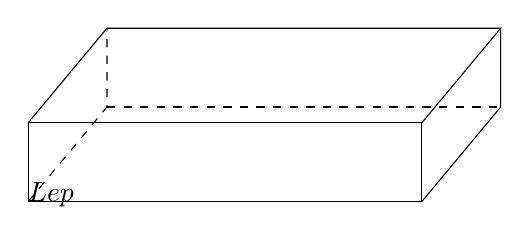
\begin{tikzpicture}
      % Parallelepipede
      \draw (0,0)--(5,0)--(5,1)--(0,1)--(0,0); % face
      \draw (0,1)--(1,2.2)--(6,2.2)--(5,1); % haut
      \draw (5,0)--(6,1.2)--(6,2.2); % côté
      % Perspective
      \draw[dashed] (0,0)--(1,1.2)--(1,2.2); % côté
      \draw[dashed] (1,1.2)--(6,1.2); % fond
      % Legendes
      \tikzVecteur*(0, -0.25) (5,0) {$L$}[below]
      \tikzVecteur*(-0.25,0) (0,1){$e$}[left]
      \tikzVecteur*(5.25, -0.1) (1, 1.2){$p$}[right]
    \end{tikzpicture}
  \end{multicols}
  Si $L$, $p$ et $e$ sont mesurées en \unit{\cm},
  le résultat s’exprimera en \unit{\cubic\cm}.
\end{doc}

\mesure Mesurer la masse volumique d'un échantillon à l'aide du matériel disponible.

\question{
  En utilisant le document~\ref{doc:TP3_proprietes_metaux}, déterminer la nature de l'échantillon.
}{
  On a mesuré un volume $V = 10,0 \times 2,0 \times \qty{0.2}{\centi\m\cubed} = \qty{4,0}{\centi\m\cubed}$ et une masse $m = \qty{34,0}{\g}$.
  L'échantillon a donc une masse volumique 
  \begin{equation*}  
    \rho
    = \dfrac{30,0}{4,0}\unit{\g/\cubic\centi\m}
    = \qty{7,5}{\g/\cubic\centi\m}
  \end{equation*}

  Comme l'échantillon est brillant et gris, on en déduit qu'on a du fer.
}[2]



%%%% Contexte 2
\begin{importants}
  Les eaux minérales sont des mélanges homogène contenant plusieurs ions de nature et de masses différentes.
  Les eaux minérales sont en général impropre à une consommation régulière, mais elles peuvent servir dans des régimes spécifiques.
  
  \hspace{8pt} \problematique{Comment déterminer les ions présents dans des eaux minérales ?}
\end{importants}



%%%% documents
\begin{doc}{Composition de trois eaux minérales}{doc:TP3_composition_eau}
  \newcommand{\vichyStYorre}{
  \important{Vichy St Yorre} \\
  \begin{tblr}{
    colspec = {l | r}, hlines, hline{1} = {white},
    column{2} = {couleurSec-50}, row{1} = {couleurSec-100},
  }
    \SetCell[c=2]{c} Minéralisation : \unit{\mg} pour \qty{1}{\litre} \\
    \ionBicarbonate & \num{4368} \\
    \ionChlorure    & \num{322}  \\
    \ionSodium      & \num{1708} \\
    \ionSulfate     & \num{174}  \\
    \ionPotassium   & \num{110}  \\
    \ionCalcium     & \num{90}   \\
    \ionFluorure    & \num{1}    \\
    \ionMagnesium   & \num{11}   \\
  \end{tblr}
}
    
\newcommand{\montRoucous}{
  \important{Mont Roucous \phantom{y}} \\
  \begin{tblr}{
    colspec = {l | r}, hlines, hline{1} = {white},
    column{2} = {couleurSec-50}, row{1} = {couleurSec-100},
  }
    \SetCell[c=2]{c} Minéralisation : \unit{\mg} pour \qty{1}{\litre} \\
    \ionBicarbonate & \num{1} \\
    \ionChlorure    & \num{2}  \\
    \ionSodium      & \num{3,2}  \\
    \ionSulfate     & \num{6,9}  \\
    \ionFluorure    & < \num{0,1}  \\
    \ionCalcium     & \num{2,7}  \\
    \ionNitrate     & \num{1,8}  \\
    \ionMagnesium   & \num{0,3}  \\
  \end{tblr}
}

\newcommand{\cristalline}{
  \important{Cristalline \phantom{y}} \\
  \begin{tblr}{
    colspec = {l | r}, hlines, hline{1} = {white},
    column{2} = {couleurSec-50}, row{1} = {couleurSec-100},
  }
    \SetCell[c=2]{c} Minéralisation : \unit{\mg} pour \qty{1}{\litre} \\
    \ionBicarbonate & \num{228} \\
    \ionChlorure    & \num{15}    \\
    \ionSodium      & \num{8,4}  \\
    \ionSulfate     & \num{11}  \\
    \ionPotassium   & \num{2,3}     \\
    \ionCalcium     & \num{549}   \\
    \ionNitrate     & < \num{1}   \\
    \ionMagnesium   & \num{6,9}   \\
  \end{tblr}
}

\newcommand{\volvic}{
  \important{Volvic \vphantom{y}} \\
  \begin{tblr}{
    colspec = {l | r}, hlines, hline{1} = {white},
    column{2} = {couleurSec-50}, row{1} = {couleurSec-100},
  }
    \SetCell[c=2]{c} Minéralisation : \unit{\mg} pour \qty{1}{\litre} \\
    \ionBicarbonate & \num{65,3} \\
    \ionChlorure    & \num{8,4}  \\
    \ionSodium      & \num{9,4}  \\
    \ionSulfate     & \num{6,9}  \\
    \ionPotassium   & \num{5,7}  \\
    \ionCalcium     & \num{9,9}  \\
    \ionNitrate     & \num{6,3}  \\
    \ionMagnesium   & \num{6,1}  \\
  \end{tblr}
}

\newcommand{\hepar}{
  \important{Hépar \vphantom{y}} \\
  \begin{tblr}{
    colspec = {l | r}, hlines, hline{1} = {white},
    column{2} = {couleurSec-50}, row{1} = {couleurSec-100},
  }
    \SetCell[c=2]{c} Minéralisation : \unit{\mg} pour \qty{1}{\litre} \\
    \ionBicarbonate & \num{383,7} \\
    \ionChlorure    & \num{11}    \\
    \ionSodium      & \num{14,2}  \\
    \ionSulfate     & \num{1479}  \\
    \ionPotassium   & \num{4}     \\
    \ionCalcium     & \num{549}   \\
    \ionNitrate     & \num{4,3}   \\
    \ionMagnesium   & \num{119}   \\
  \end{tblr}
}
  \begin{multicols}{3}
    \centering
    %
    \vichyStYorre
    %
    \montRoucous
    %
    \cristalline
  \end{multicols}
\end{doc}


%%%%
\begin{doc}{Tests caractéristiques de certains ions}{doc:TP3_tests_ions}
  \begin{center}
    \begin{tableau}{| c | c | c |}
      Ion à tester &
      Réactif utilisé &
      Résultat du test positif \\
      %
      \ionChlorure &
      Solution de nitrate d'argent &
      Précipité blanc, noircit* \\
      %
      \ionSulfate &
      Solution de chlorure de baryum &
      Précipité blanc \\
      %
      \ionCalcium &
      Solution d'oxalate d'ammonium &
      Précipité blanc \\
      %
      \ionMagnesium &
      Solution d'hydroxyde de sodium &
      Précipité blanc
    \end{tableau}
    
    \bigskip
    * Le précipité blanc noircit à la lumière.
  \end{center}
\end{doc}


%%%%
On a trois béchers (A, B, C) contenant des eaux minérales, que vous voulez identifier.

\mesure
Réaliser le protocole suivant :
\begin{protocole}
  \item Verser dans 4 tubes à essais quelques \unit{\mL} d'eau d'un bécher.
  \item Réaliser un test différent dans chaque tube à essais à l'aide des 4 réactifs.
  \item Noter si un précipité se forme et son abondance dans le tableau suivant ($-$, $+$, $++$, $+++$).
  \item Répéter pour les deux autres bécher.
\end{protocole}

\begin{center}
  \begin{tableau}{|l | c | c | c|}
    Test réalisé & Bécher A & Bécher B & Bécher C \\
    Nitrate d'argent    & & & \\
    Chlorure de baryum  & & & \\
    Oxalate d'ammonium  & & & \\
    Hydroxyde de sodium & & &
  \end{tableau}
\end{center}

\question{
  En utilisant les documents~\ref{doc:TP3_composition_eau} et~\ref{doc:TP3_tests_ions}, donner l'eau minérale contenue dans chaque bécher.
}{
  
}[3]

% %%%%
\teteSndCorp

%%%% titre
\vspace*{-36pt}
\numeroActivite{1}
\titreActivite{Composition de l'atmosphère}


%%%% objectifs
\begin{objectifs}
  \item Comprendre comment on décrit la composition d'un mélange.
  \item Connaître la composition de l'air.
\end{objectifs}

\begin{contexte}
  L'atmosphère est un mélange de plusieurs gaz : dioxygène, diazote, dioxyde de carbone, etc.
  
  \problematique{
    Comment décrire la composition d'un mélange ?
  }
\end{contexte}


%%%% docs
\begin{doc}{Fraction volumique}{doc:A1_fraction_volumique}
  Soit une espèce chimique $E$ de volume $V_E$, dans un mélange de volume total $V$.
  La \important{proportion} ou \important{fraction volumique} de l'espèce chimique $E$ est
  \begin{equation*}
    p_{v}(E) = \frac{V_E}{V}
  \end{equation*}
  C'est une grandeur sans unité, comprise entre 0 et 1.
  On peut aussi l'exprimer en pourcentage, compris entre \qty{0}{\percent} et \qty{100}{\percent}.
  Par définition $\qty{10}{\percent} = \dfrac{10}{100} = \num{0,10}$.
\end{doc}

%%
\begin{doc}{Composition de l'atmosphère}{doc:A1_composition_atmo}
  \begin{importants}
    L’air contient \texteTrou[0.1]{\qty{78}{\percent}} de diazote \chemfig{N_2} et \texteTrou[0.1]{\qty{21}{\percent}} de dioxygène \chemfig{O_2}.
    Les autres gaz qui composent l’air sont l’argon \chemfig{Ar} (\qty{0,9}{\percent}),
    le dioxyde de carbone \chemfig{CO_2} (\qty{0,04}{\percent}),
    les gaz nobles et le méthane \chemfig{CH_4} (\qty{0,0002}{\percent}).
  \end{importants}
\end{doc}


%%%%
\question{
  Calculer le volume occupé par le diazote \chemfig{N_2} dans une salle de cours de \qty{600}{\metre\cubed}.
}{
  Le diazote occupe \qty{78}{\percent} du volume, soit $V_{\chemfig{N_2}} = 0,78 \times \qty{600}{\metre\cubed} = \qty{468}{\metre\cubed}$.
}{2}

\question{
  Même question pour le dioxygène \chemfig{O_2}.
}{
  Cette fois $V_{\chemfig{O_2}} = 0,21 \times \qty{600}{\metre\cubed} = \qty{126}{\metre\cubed}$.

}{2}

\begin{doc}{Respiration et dioxyde de carbone}{doc:A1_respiration}
  Quand on respire, on inspire du dioxygène \chemfig{O_2} qui est transformé en dioxyde de carbone \chemfig{CO_2} que l'on expire.

  Pendant une séance de cours d'une heure, le volume de dioxyde de carbone \chemfig{CO_2} double à cause de la respiration, si la salle n'est pas aérée.
\end{doc}

\question{
  Calculer la proportion volumique de dioxyde de carbone \chemfig{CO_2} après une heure de cours.
}{
  Le volume de dioxyde de carbone a doublé, on a donc une proportion deux fois plus élevée, soit \qty{0,08}{\percent}.
}{3}


%%
\begin{doc}{Fraction massique}{doc:A1_fraction_massique}
  Soit une espèce chimique $E$ de masse $m_E$, dans un mélange de masse totale $m$.
  La \important{proportion} ou \important{fraction massique} de l'espèce chimique $E$ est
  \begin{equation*}
    p_{m}(E) = \frac{m_E}{m}
  \end{equation*}
  C'est une grandeur sans unité, comprise entre 0 et 1.
  On peut aussi l'exprimer en pourcentage, compris entre \qty{0}{\percent} et \qty{100}{\percent}.
\end{doc}

\begin{doc}{Cloche en bronze}{doc:A1_cloche_bronze}
  \begin{wrapfigure}[5]{r}{0.2\linewidth}
    \vspace*{-31pt}
    \centering
    \image{0.7}{images/photos/cloche_bronze.png}
  \end{wrapfigure}
  
  Les cloches traditionnelles des temples coréens sont en bronze.
  Le bronze est un \important{alliage,} un mélange homogène entre deux métaux.
  
  Le bronze est constitué de \qty{20}{\percent} d'étain \chemfig{Sn} et de \qty{80}{\percent} de cuivre \chemfig{Cu} en masse.

  Une cloche traditionnelle pèse plusieurs centaines de kilogramme.
\end{doc}


\question{
  Exprimer les proportions massiques du cuivre et de l'étain dans une cloche en bronze sous la forme d'une division entre deux entiers les plus petits possibles.
}{
  $\qty{20}{\percent} = \dfrac{20}{100} = \dfrac{1}{5}$ pour l'étain.
  $\qty{80}{\percent} = \dfrac{80}{100} = \dfrac{4}{5}$ pour le cuivre.
}{3}

\question{
  Calculer la masse cuivre dans une cloche traditionnelle de masse $m = \qty{500}{\kg}$
}{
  La masse de cuivre vaut $0,8 \times \qty{500}{\kg} = \qty{400}{\kg}$.
}{2}

\question{
  Même question pour l'étain.
}{
  La masse d'étain vaut $0,2 \times \qty{500}{\kg} = \qty{100}{\kg}$.
}{2}

\question{
  Est-ce que l'on pourrait calculer les fractions volumiques de cuivre et d'étain à partir des fractions massiques ?
}{
  Non, car on ne sait pas quel est le volume de la cloche, ni quels sont les volumes de cuivre et d'étain dans la cloche.
}{1}

% %%%% début de la page
\teteSndCorp

%%%% titre
\nomPrenomClasse
\titreTP{Séparer et identifier des espèces chimiques}


%%%% objectifs
\begin{objectifs}
  \item Réaliser et analyser une Chromatographie sur Couche Mince.
\end{objectifs}


%%%% evaluation
\begin{tableauCompetences}
  VAL & Comparer des valeurs mesurées avec des valeurs de références.
\end{tableauCompetences}



%%%% contexte
\begin{contexte}
  En Europe, les colorants alimentaires sont désignés par un préfixe E suivi d'un numéro.
  Ces colorants se retrouvent dans de nombreux produits.
  
  On cherche à déterminer les colorants présent dans des M\&M's à l'aide d'une \important{Chromatographie sur Couche Mince (CCM).}
\end{contexte}


%%%% document
\begin{doc}{Chromatographie sur Couche Mince (CCM)}{doc:TP4_CCM}
  \begin{wrapfigure}{l}{0.45\linewidth}
    \centering
    \vspace*{-16pt}
    \image{0.9}{images/chimie/CCM/CCM.png} \\
    \legende{Schéma expérimental d'une CCM.}
  \end{wrapfigure}

  La \important{chromatographie sur couche mince (CCM)} permet de séparer et d'identifier des espèces chimiques dans un mélange.

  Le principe est le suivant : on dépose les espèces à identifier sur une plaque, appelée \important{phase stationnaire.} On fait tremper une partie de la plaque dans un liquide appelé \important{éluant}.
  
  Par capillarité, l'éluant va monter le long de la plaque et les espèces déposées sur la plaque vont être poussées par l'éluant pendant sa montée.
  
  En fonction de leurs propriétés, les espèces chimiques seront poussées plus ou moins haut sur la plaque, ce qui permettra de les identifier.
  La fiche ainsi formée est appelée un \important{chromatogramme}.
\end{doc}

%%%%
\begin{doc}{Réalisation d'une CCM}{doc:TP4_protocole_CCM}
  \begin{multicols}{3}
    \begin{center}
      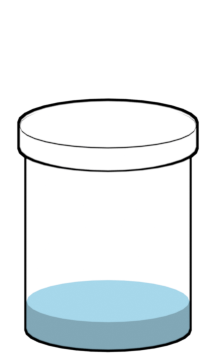
\includegraphics[height=0.2\textheight]{images/chimie/CCM/CCM_protocole0001.png} \\      
      Remplir la cuve à CCM avec environ \qty{1}{\cm} d'éluant.
    \end{center} 
    
    \begin{center}
      
\includegraphics[height=0.2\textheight]{images/chimie/CCM/CCM_protocole0002.png} \\      
      Tracer au crayon à papier un trait à \qty{1}{\cm} du bord inférieur.
    \end{center}
  
    \begin{center}
      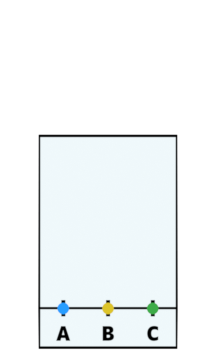
\includegraphics[height=0.2\textheight]{images/chimie/CCM/CCM_protocole0003.png} \\      
      À l'aide d'un cure-dent, déposer chaque échantillon sur un emplacement bien délimité.
    \end{center}
  \end{multicols}
  
  \bigskip
  
  \begin{multicols}{2}
    \begin{center}
      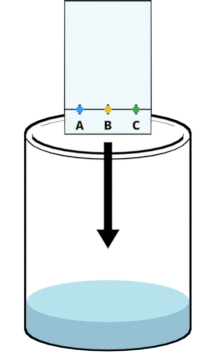
\includegraphics[height=0.2\textheight]{images/chimie/CCM/CCM_protocole0004.png}
      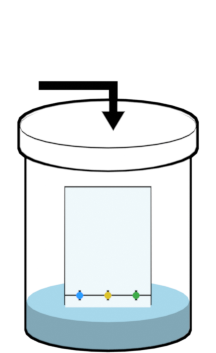
\includegraphics[height=0.2\textheight]{images/chimie/CCM/CCM_protocole0005.png} \\      
      Poser doucement la plaque dans la cuve en la tenant par les côtés et fermer la cuve.
      \important{Il ne faut jamais déplacer la cuve} et attendre que l'éluant monte.
    \end{center}

    \begin{center}
      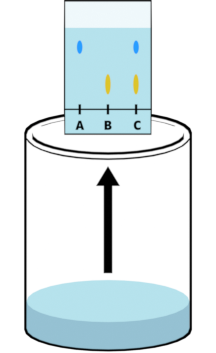
\includegraphics[height=0.2\textheight]{images/chimie/CCM/CCM_protocole0006.png} \\      
      Quand le front de l'éluant s'approche du haut, sortir la plaque.
      Tracer une ligne indiquant la hauteur où l'éluant est monté.
    \end{center}
  \end{multicols}
\end{doc}


%%%% questions
\mesure
Placer un M\&M's dans chaque tube à essais et les recouvrir d'eau.
Attendre que le colorant se soit dissous dans l'eau et récupérer les M\&M's.

\mesure
Réaliser le protocole du document~\ref{doc:TP4_protocole_CCM}, avec un dépôt de colorant jaune, un dépôt de colorant bleu et deux dépôts des solutions préparées précédemment.

\mesure
Schématiser le chromatogramme obtenu, en indiquant clairement les différentes tâches, la ligne de dépôt et le front de l'éluant.
\pasCorrection{\vfill}

\question{
  Pourquoi doit-on placer la ligne de dépôt au dessus du niveau de l'éluant ?
}{
  Si on la place en dessous, le dépôt va se diluer dans l'éluant et ne montera pas sur la plaque.
}[2]

\question{
  Pourquoi ne doit-on pas déplacer la cuve pendant la montée de l'éluant ?
}{
  Si on déplace la cuve, l'éluant va monter de manière irrégulière, ce qui va fausser l'analyse des résultats.
}[2]


%%%%
\pasCorrection{\newpage}
\begin{doc}{Lecture d'un chromatogramme}{doc:TP4_lecture_chromato}
  \separationBlocs{
    \begin{listePoints}
      \item \important{Lecture verticale :} si le dépôt d'un échantillon se sépare en plusieurs tâches, il s'agit d'un mélange. 
      Le nombre de tâches indique le nombre d'espèces chimiques qui composent le mélange.
      \item \important{Lecture horizontale :} sur une même plaque, une même espèce chimique migre toujours à la même hauteur. 
      Et donc si deux tâches sont à \important{la même hauteur, alors elles sont la même espèce chimique.}
    \end{listePoints}
    \vfill \strut
  }{
    \centering
    \vspace*{-20pt}
    \image{0.8}{images/chimie/CCM/chromatogramme.png} \\
    \legende{schéma d'un chromatogramme}
  }
\end{doc}

%%%%
\begin{doc}{Colorants alimentaires}{doc:TP4_colorants_alimentaire}
  \begin{listePoints}
    \item \important{E102 : jaune de tartrazine.} Son usage doit s'accompagner en France de la mention « peut avoir des effets indésirables sur l'activité et l'attention chez les enfants ».
    \item \important{E133 : bleu brillant.} Un enfant de 40 kg peut ingérer jusqu'à \qty{240}{\mg} de bleu brillant en une journée. Au-delà le conseil européen indique que ce produit peut être toxique.
  \end{listePoints}
\end{doc}

\question{
  En analysant le chromatogramme à l'aide du document~\ref{doc:TP4_lecture_chromato}, indiquer si les échantillons sont des corps purs ou des mélanges.
}{
  Pour le bleu et le jaune, on a des corps purs (une seule tâche).
  Pour le vert on a un mélange, car le dépôt s'est séparé en deux tâches.
}[5]

\question{
  En utilisant le chromatogramme, donner la composition des colorants présents sur la couche externe des M\&M's.
}{
  Le jaune et le bleu du M\&M's montent à la même hauteurs que les dépots de colorant jaune E102 et bleu E133, ce sont donc les mêmes espèces chimiques.
}[5]


\pasCorrection{\newpage}

\important{\large Composition des huiles essentielle d'orange et de citron}

%%%% Contexte
\begin{contexte}
  Les huiles essentielles sont obtenues à partir de végétaux pressés ou par distillation fractionnée.
  Les huiles essentielles sont riches en molécules odorantes.
  
  \problematique{
    Comment décrire la composition d'une huile essentielle à l'aide d'une CCM ?
  }
\end{contexte}


%%%% docs
\separationBlocs{
  %%
  \begin{doc}{Huile essentielle de citron et d'orange}{doc:TP4_huile_essentielle}
    L'huile essentielle d'orange (HEO) et l'huile essentielle de citron (HEC)
    sont obtenues en pressant les zestes d'une orange et d'un citron respectivement.
  \end{doc}
}[0.31]{
  %%
  \begin{doc}{Odorat et molécules odorantes}{doc:TP4_molecules_odorantes}
    Chez les humains, Les molécules odorantes sont captées par des neurones de l’épithélium olfactif,
    puis ces neurones transmettent l'information nerveuse au cerveau qui y associe une odeur.
  
    Voilà quelques exemples de molécules odorantes :
    \begin{listePoints}
      \item le \important{limonène} (Lim), est associé à une odeur d'orange.
      \item le \important{linalol} (Lin), est associé à une odeur fraiche et florale.
      \item le \important{géraniol} (G), est associé à une odeur de rose.
      \item le \important{citral} (Ci), est associé à une odeur de citron.
    \end{listePoints}
  \end{doc}
}[0.69]


%%%%
\question{
  Quelles molécules odorantes peut-on trouver dans l'huile essentiel de citron et d'orange ?
}{
  D'après les descriptions du document~\ref{doc:TP4_molecules_odorantes},
  on s'attend à trouver du limonène dans l'huile essentielle d'orange et du citral dans l'huile essentielle de citron.
}[2]

\begin{doc}{Résultat d'une CCM}{doc:TP4_HEC_HEO}
  On a réalisé deux CCM pour déterminer la composition des huiles essentielles d'orange et de citron.
  \begin{center}
    \image{0.25}{images/donnees/chromato_HEC}
    \image{0.25}{images/donnees/chromato_HEO}
  \end{center}
\end{doc}

\question{
  En analysant les chromatogrammes, donner la composition des huiles essentielles de citron et d'orange (HEC et HEO).
}{
  On trouve du limonène, du géraniol et du citral dans l'HEC (tâches à la même hauteur).
  On trouve du limonène et du géraniol dans l'HEO.
}[5]

% %%%%
\teteSndCorp

%%%% titre
%\vspace*{-36pt}
\titreActivite{Mesure de la masse volumique de l'air}


%%%% objectifs
\begin{objectifs}
  \item Calculer la masse volumique de l'air.
\end{objectifs}

\begin{contexte}
  L'atmosphère est un mélange de plusieurs gaz : dioxygène, diazote, dioxyde de carbone, etc.
  
  \problematique{
    Comment calculer la masse volumique de l'air à partir de sa composition ou d'une expérience ?
  }
\end{contexte}


%%%% docs
\begin{doc}{Mesure de la masse volumique de l'air}{doc:A2_mesure_densite_air}
  \begin{wrapfigure}{r}{0.1\linewidth}
    \vspace*{-29pt}
    \qrcode{https://www.youtube.com/watch?v=isEo51ncsKU&t=26s}
  \end{wrapfigure}
  On peut mesurer la masse volumique de l'air en dégonflant un ballon dans une bouteille d'eau.
  La bouteille d'eau permet de mesurer le volume d'air expulsé.
  En pesant le ballon avant et après le dégonflage, on peut calculer la masse d'air expulsée.
\end{doc}

\numeroQuestion 
Schématiser les 3 étapes de l'expérience réalisée.
\pasCorrection{\vspace*{200pt}}
\correction{
  Schéma du ballon sur la balance avec $m_1$,
  schéma du ballon vidé dans une éprouvette graduée avec l'air qui prend la place de l'eau,
  schéma du ballon sur la balance avec $m_2$.
}

\numeroQuestion
Remplir le tableau ci-dessous 
\begin{tableau}{|c |c |c |c |}
  Grandeur & Masse du ballon plein $m_1 $ & Masse du ballon dégonflé $m_2$ & Volume d'air expulsé $V$ \\
  \SetCell{couleurSec-50} Valeur & \correction{\qty{483,2}{\g}} & \correction{\qty{481,4}{\g}} & \correction{\qty{1,5}{\litre}}
\end{tableau}

\question{
  Calculer la masse volumique mesurée $\rho_\text{mes}(\text{air})$.
}{
  La masse d'air expulsée est $m = m_2 - m_1 = \qty{1,8}{\g}$, soit une masse volumique
  \begin{equation*}
    \rho = \dfrac{m}{V} = \frac{1,8}{1,5} \unit{\g\per\litre} = \qty{1,2}{\g\per\litre}
  \end{equation*}
}[3]

%%
\begin{doc}{Masse volumique d'un mélange}{doc:A2_composition_atmo}
  Pour un mélange de gaz, la masse volumique du mélange est simplement la somme des masses volumique de chaque gaz pondérée par la fraction volumique de chaque gaz du mélange.

  Pour l'air, on aura donc
  \begin{equation*}
    \rho(\text{air}) = p_v(\chemfig{O_2}) \rho(\chemfig{O_2}) + p_v(\chemfig{N_2}) \rho(\chemfig{N_2}) + p_v(\chemfig{Ar}) \rho(\chemfig{Ar}) + p_v(\chemfig{CO_2}) \rho(\chemfig{CO_2})
  \end{equation*}
\end{doc}

\pasCorrection{\newpage}
\question{
  Rappeler les fractions volumique des gaz composant l'air (\chemfig{O_2}, \chemfig{N_2}, \chemfig{CO_2}, \chemfig{Ar}).
}{
  $p_v(\chemfig{O_2})  = \qty{21}{\percent}$, 
  $p_v(\chemfig{N_2})  = \qty{78}{\percent}$, 
  $p_v(\chemfig{CO_2}) = \qty{0,04}{\percent}$, 
  $p_v(\chemfig{Ar})   = \qty{0,9 }{\percent}$, 
}[2]

\begin{doc}{Masse volumique des gaz composant l'air}{doc:A2_masse_volumique_gaz}
  \textbf{Données :}
  \begin{listeTirets}
    \item Masse volumique du \chemfig{CO_2} gazeux : $\rho(\chemfig{CO_2}) = \qty{1,87}{\g/\litre}$.
    \item Masse volumique du \chemfig{O_2}  gazeux : $\rho(\chemfig{O_2})  = \qty{1,35}{\g/\litre}$.
    \item Masse volumique du \chemfig{N_2}  gazeux : $\rho(\chemfig{N_2})  = \qty{1,18}{\g/\litre}$.
    \item Masse volumique de \chemfig{Ar}   gazeux : $\rho(\chemfig{Ar})   = \qty{1,78}{\g/\litre}$.
  \end{listeTirets}
\end{doc}


%%%%
\question{
  Calculer la masse volumique théorique de l'air $\rho_\text{theo} (\text{air})$.
}{
  $\rho_\text{theo} (\text{air}) 
  = (0,21\times 1,35 + 0,78\times 1,18 + 0,0004\times 1.87 + 0.009\times 1.78) \unit{\g/\litre}
  = \qty{1.22}{\g/\litre}$
}[4]

\question{
  Comparer la valeur théorique et la valeur mesurée. Est-ce qu'elles sont égales ? Est-ce qu'elles sont cohérentes ?
}{
  On trouve deux valeurs légèrement différentes, \qty{1,2}{\g/\litre} et \qty{1,22}{\g/\litre}, mais elles sont cohérentes avec la précision des mesures réalisées pendant l'expérience.
}[2]


%% Solutions
% %%%% début de la page
\teteSndSolu

%%%% titre
\vspace*{-36pt}
\titreTP{Dosage du sucre par étalonnage}

%%%% objectifs
\begin{objectifs}
  \item Apprendre le vocabulaire sur les solutions.
  \item Comprendre la notion de concentration massique
  \item Comprendre le principe de la dilution et de la dissolution
\end{objectifs}


%%%% contexte
\begin{contexte}
  Le sucre couramment présent dans notre alimentation est le saccharose.
  Cette espèce chimique peut entraîner des risques pour la santé si on en consomme trop.
  Il est donc important de pouvoir déterminer la quantité de sucre consommée par jour.

  \problematique{Comment déterminer la masse de saccharose présent dans un sirop ?}
\end{contexte}


%%%% documents
\begin{doc}{Solution, solvant et soluté}{doc:TP1_solution}
  \begin{importants}
    \chevron Une \important{solution} est un mélange homogène. \\
    Le \important{solvant} est le composant majoritaire du mélange.
    Les \important{solutés} sont les espèces qui sont dispersées dans le solvant.
  \end{importants}
  
  \begin{center}
    \important{Solvant + Soluté(s) = Solution}
  \end{center}
  
  \begin{importants}
    On parle de \important{solution aqueuse} si le solvant est l'eau \chemfig{H_2 O}.
  \end{importants}
\end{doc}

\begin{doc}{Composition d'un sirop}{doc:TP1_sirop}
  Le constructeur annonce que le sirop est composé d'\textit{eau}, de \textit{sucre} de \textit{jus de citron} et d'\textit{acide citrique} principalement.
\end{doc}


\question{
  Donner le solvant et les solutés présents dans le sirop.
}{
  Le solvant du sirop est l'eau, les solutés sont le sucre, le jus de citron et l'acide citriques.
}[2]


%%%%
\begin{doc}{Concentration en soluté}{doc:TP1_concentration}
  \begin{importants}
    La \important{concentration massique $\mathbf{c}$} mesure la quantité de soluté présent dans une solution.
    C'est le rapport de la masse $m$ de \important{soluté} dissous dans le volume $V$ de la \important{solution}
    \begin{equation*}
      c = \frac{m_\text{soluté}}{V_\text{solution}}
    \end{equation*} 
  \end{importants}
  % \attention Il faut bien distinguer \important{concentration massique} et \important{masse volumique}.
  % La concentration mesure la masse de soluté contenue dans une solution.
  % La masse volumique mesure la masse d'un échantillon contenue dans un volume donné.
\end{doc}


\begin{doc}{Dissolution du sucre dans l'eau}{doc:TP1_protocole_dissolution}
  \begin{protocole}
      \item Peser une masse donnée de sucre avec une balance de précision.
      \item Mettre le sucre dans une fiole jaugée de 50 mL.
      \item Compléter la fiole jaugée jusqu'à mi-hauteur avec de l'eau distillée, agiter.
      \item Compléter jusqu'au trait de jauge avec de l'eau distillée.
      \item Verser le mélange dans un bêcher de 100 mL.
  \end{protocole}
\end{doc}


%%%% questions
\newpage
\vspace*{-28pt}

\mesure
En utilisant le Document~\ref{doc:TP1_protocole_dissolution}, préparer un mélange de \qty{50}{\ml} d'eau et de de sucre.

\mesure
Mesurer et noter la masse volumique du mélange préparé $\rho =$ \texteTrou[0.1]{\qty{0,15}{\g/\ml}}

\question{
  Calculer la concentration massique de sucre dans la solution aqueuse préparé.
}{
  Avec une masse de sucre de $\qty{10}{\g}$, on a une concentration massique 
  \begin{equation*}
    c = \dfrac{\qty{10}{\g}} {\qty{50}{\ml}}
    = \qty{0,2}{\g/\ml}
  \end{equation*}
}[1]


%%%%
\begin{doc}{Mesure de concentration}{doc:TP1_dosage}
  \begin{importants}
    On parle de \important{dosage} quand on mesure la concentration d'une espèce chimique présente dans une solution.
  \end{importants}
  \begin{importants}
    Un \important{dosage par étalonnage} consiste à déterminer la concentration d’une espèce chimique en comparant une grandeur physique caractéristique de la solution, à la même grandeur physique mesurée pour des solutions étalon.
  \end{importants}
\end{doc}
 
\numeroQuestion 
En utilisant le papier millimétré, tracer la masse volumique en fonction de la concentration massique de sucre dans l'eau.

\numeroQuestion
En déduire la concentration massique de sucre dans la sirop $c_\text{sirop} =$ \texteTrou[0.1]{\qty{0,6}{\g/\ml}}


%%%%
\begin{doc}{Principe d'une dilution}{doc:TP1_principe_dilution}
  \begin{wrapfigure}[5]{r}{0.5\linewidth}
    \vspace*{-16pt}
    \centering
    \begin{multicols}{4}
    \image{1.1}{images/chimie/protocoles/dissoDilu0007} \\[0pt]
    \footnotesize{$S_0$}
    
    \image{1.1}{images/chimie/protocoles/dissoDilu0008}
    
    \image{1.1}{images/chimie/protocoles/dissoDilu0010}
    
    \image{1.1}{images/chimie/protocoles/dissoDilu0011} \\[0pt]
    \footnotesize{$S_1$}
    \end{multicols}
  \end{wrapfigure}
  \vAligne{-40pt}
  
  \begin{importants}
    Le principe de la \important{dilution} est de \important{diminuer la concentration} en soluté dans une solution en rajoutant du \important{solvant.}
  \end{importants}
  La solution de départ est appelée \important{solution mère}, notée $S_0$.
  La solution obtenue après dilution est appelée \important{solution fille}, notée $S_1$.

  Pour diluer une solution, il faut
  \begin{protocole}
    \item Prélever un volume $V_0$ de la solution à l'aide de la pipette graduée.
    Le bas du ménisque doit atteindre la graduation supérieure.
    \item Introduire la solution prélevée dans la fiole jaugée de volume $V_1$.
    \item Ajouter de l'eau distillée dans la fiole jaugée jusqu'aux $2/3$ et agiter doucement. Compléter jusqu'à ce que le bas du ménisque atteigne le trait de jauge.
    \item Fermer la fiole et l'agiter en la retournant plusieurs fois.
    \item Verser la solution fille obtenue dans un bécher.
  \end{protocole}
\end{doc}


%%%%
\begin{doc}{Facteur de dilution}{doc:TP1_dilution}  
  Le \important{facteur de dilution} est le rapport du volume de la solution fille sur le volume de la solution mère
  \begin{equation*}
    F = \frac{V_\text{1}}{V_\text{0}}
  \end{equation*}
  On dit qu'on a dilué $F$ fois une solution.
\end{doc}

\mesure 
Diluer \important{2 fois} le sirop et mesurer sa masse volumique. 

\question{
  En déduire la concentration massique en sucre.
  Que constatez-vous ?
}{
  Pour diluer 2 fois, il faut que $F = 2 = \dfrac{V_\text{1}}{V_\text{0}}$, on aura donc un volume final $V_\text{1} = 2\times V_\text{0}$ deux fois plus grand que le volume initial, avec donc une concentration massique 2 fois plus faible.

  On constate que la concentration massique a été divisée par le facteur de dilution.
}

% %%%% début de la page
\teteSndSolu

%%%% titre
\vspace*{-36pt}
\titreActivite{Mal de tête et dissolution}

%%%% objectifs
\begin{objectifs}
  \item Calculer une concentration massique.
\end{objectifs}


%%%% contexte
\begin{contexte}
  Inès, 8 ans, a mal à la tête et son père décide de lui donner du paracétamol pour la soulager, sauf qu'il ne possède que des comprimés pour adulte !

  \problematique{Comment le père va-t-il calculer la bonne dose à administrer à sa fille ?}
\end{contexte}


%%%% documents
\begin{doc}{Solution, solvant et soluté}{doc:A1_solution}
  \begin{importants}
    Une \important{solution} est un mélange homogène.
    Le \important{solvant} est le composant majoritaire du mélange.
    Les \important{solutés} sont les espèces qui sont dispersées par le solvant.
    \begin{center}
        \important{solvant + solutés = solution}
    \end{center}
  \end{importants}
\end{doc}

\begin{doc}{Le paracétamol}{doc:A1_paracétamol}
  \begin{wrapfigure}[5]{r}{0.3\linewidth}
    \vspace*{-30pt}
    \centering
    \chemname{\chemfig{!\paracetamol}}{paracétamol}
  \end{wrapfigure}
  
  Le paracétamol est un antidouleur qui peut être dangereux pour le foie s'il est consommé en trop grande quantité.
  Un comprimé pour adulte a une masse $m_1 = \qty{500}{\milli\g}$, alors qu'un comprimé pour enfant a une masse $m_2 = \qty{300}{\milli\g}$.
  
  Pour calmer le mal de tête d'Inès, le père décide qu'il va \important{dissoudre} un comprimé de paracétamol pour adulte dans un verre d'eau de volume $V_1 = \qty{25}{\centi\litre}$.
\end{doc}


\question{
  Donner le solvant et les solutés de la solution préparée par le père.
}{
  Le solvant de la solution est l'eau, le soluté est le paracétamol.
}[2]


\begin{doc}{Concentration massique}{doc:A1_concentration_massique}
  \begin{importants}
    La \important{concentration massique $\mathbf{c}$} mesure la quantité de soluté présent dans une solution.
    C'est le rapport de la masse de \important{soluté} dissous sur le volume total de la \important{solution}
    \begin{equation*}
      c = \frac{m_\text{soluté}}{V_\text{solution}}
    \end{equation*}
  \end{importants}
\end{doc}

\question{
  Convertir le volume $V_1$ de la solution en millilitre, noté \unit{\ml}.
}{
  \begin{equation*}  
    V_1 = \qty{25}{\centi\litre} = \qty{250}{\ml}
  \end{equation*}
}[1]

\question{
  Calculer la concentration $c$ en \unit{\mg/\ml} de paracétamol dans le verre d'eau.
}{
  \begin{equation*}
    c = \dfrac{m_1}{V_1}
      = \dfrac{\qty{500}{\mg}} {\qty{250}{\ml}}
      = \qty{2,0}{\mg/\ml}
  \end{equation*}
}[4]

\newpage
\question{
  Quel volume $V_2$ de la solution (du verre d'eau) Inès doit-elle boire pour avaler $m_2 = \qty{300}{\milli\g}$ de paracétamol ?
}{
  \begin{equation*}
    V_2 = \dfrac{m_2}{c}
        = \dfrac{\qty{300}{\mg}} {\qty{2,0}{\mg/\ml}}
        = \qty{150}{\ml}
        = \qty{15,0}{\centi\litre}
  \end{equation*}
}[6]

% %%%% début de la page
\teteSndSolu


%%%% titre
\vspace*{-36pt}
\titreTP{Dosage d'un antiseptique}


%%%% objectifs
\begin{objectifs}
  \item Comprendre la notion de concentration massique.
  \item Doser la quantité de permanganate de potassium présente dans du Dakin.
\end{objectifs}


%%%% contexte
\begin{contexte}
  Le Dakin est une solution antiseptique qui sert à nettoyer des plaies. Le principe actif du Dakin est stabilisé par l'ajout de permanganate de potassium \chemfig{KMnO_4}.
  Le permanganate de potassium donne une teinte violette au Dakin.
  
  \problematique{Comment mesurer la concentration en \chemfig{KMnO_4} dans le Dakin ?}
\end{contexte}


%%%%
\begin{doc}{Concentration en soluté}{doc:TP2_concentration}
  \begin{importants}
    La \important{concentration massique $\mathbf{c}$} mesure la quantité de soluté présent dans une solution.
    C'est le rapport de la masse $m$ de \important{soluté} dissous dans le volume $V$ de la \important{solution}
    \begin{equation*}
      c = \frac{m_\text{soluté}}{V_\text{solution}}
    \end{equation*}
  \end{importants}
\end{doc}


%%%%
\begin{doc}{Dakin}{doc:TP2_dakin}
  Le Dakin est une solution aqueuse d'hypochlorite de sodium \chemfig{Na ClO}.
  Du permanganate de potassium \chemfig{K MnO_4} est ajouté à la solution, pour qu'elle ne soit pas dégradée par l'exposition au rayonnement UV du Soleil.
  
  \fleche Sur une bouteille de Dakin il est indiqué que la concentration de \chemfig{KMnO_4} vaut $\approx \qty{0,01}{\g/\litre}$.
\end{doc}

%
\question{
  Donner le solvant et les solutés de la solution de Dakin.
}{
  Le solvant est l'eau, les solutés sont le permanganate de potassium et l'hypochlorite de sodium.
}[2]


%%%%
\begin{doc}{Mesure de concentration d'une solution colorée}{doc:TP2_dosage}  
  \begin{importants}
    Une \important{échelle de teinte} permet de mesurer la concentration d'un soluté coloré.
  \end{importants}

  La teinte d'une solution est proportionnelle à la concentration en soluté.
  On prépare une série de solutions \important{étalons} dont on connaît la concentration et on compare leur teinte avec la solution dont on veut mesurer la concentration.
  
  \attention Il faut comparer les teintes avec des verreries identiques, la teinte s'assombrit avec l'épaisseur.
\end{doc}


%%%%
\begin{doc}{Protocole d'une dilution}{doc:TP2_protocole_dilution}
  \begin{wrapfigure}[5]{r}{0.5\linewidth}
    \vspace*{-20pt}
    \centering
    \begin{multicols}{4}
    \image{1.1}{images/chimie/protocoles/dissoDilu0007} \\[0pt]
    \footnotesize{$S_0$}
    
    \image{1.1}{images/chimie/protocoles/dissoDilu0008}
    
    \image{1.1}{images/chimie/protocoles/dissoDilu0010}
    
    \image{1.1}{images/chimie/protocoles/dissoDilu0011} \\[0pt]
    \footnotesize{$S_1$}
    \end{multicols}
  \end{wrapfigure}
  \vAligne{-40pt}
  
  \begin{importants}
    La \important{dilution} est la \important{diminution de la concentration} en soluté d'une solution en rajoutant du \important{solvant.}
  \end{importants}
  La solution de départ est appelée \important{solution mère}, notée $S_0$.
  La solution obtenue après dilution est appelée \important{solution fille}, notée $S_1$.

  Pour diluer une solution, il faut
  \begin{protocole}
    \item Prélever un volume $V_0$ de la solution à l'aide d'une pipette graduée.
    \important{Le bas du ménisque} doit atteindre la graduation supérieure.
    \item Introduire la solution prélevée dans la fiole jaugée de volume $V_1$.
    \item Ajouter de l'eau distillée dans la fiole jaugée jusqu'aux $2/3$ et agiter doucement.
    Compléter jusqu'à ce que \important{le bas du ménisque} atteigne le trait de jauge.
    \item Fermer la fiole et l'agiter en la retournant plusieurs fois.
    \item Verser la solution fille obtenue dans un bécher.
  \end{protocole}
\end{doc}

%%%%
\begin{doc}{Facteur de dilution}{doc:TP1_dilution}  
  Le \important{facteur de dilution} est le rapport du volume de la solution fille sur le volume de la solution mère et il est égal au rapport des concentrations des solutions mère et fille.
  \begin{equation*}
    F = \dfrac{V_1}{V_0} = \dfrac{c_0}{c_1}
  \end{equation*}
\end{doc}


%
\question{
  On souhaite réaliser une échelle de teinte composée de 4 solutions étalon pour mesurer la concentration de permanganate de potassium dans le Dakin.

  \begin{center}
    \begin{tblr}{c | X[1,c] | X[1,c] | X[1,c] | X[1,c]}
      Solution étalon & 1 & 2 & 3 & 4 \\ \hline
      Concentration (\unit{\g/\litre}) & \correction{\num{0,05}} & \correction{\num{0,025}} & \correction{\num{0,0125}} & \correction{\num{0,0063}} 
    \end{tblr}
  \end{center}
  
  Calculer le facteur de dilution entre les différentes solutions.
}{
  On divise par deux la concentration pour passer de la solution 1 à la solution 2, de la 2 à la 3 et de la solution 3 à la solution 4.
  Donc le facteur de dilution est $F = 2$.
}[1]

%
\question{
  Justifier l’intervalle des concentrations proposées pour l’échelle de teinte, à partir de la valeur attendue de la concentration en permanganate de potassium.
}{
  La valeur attendue de la concentration ($c = \qty{0,01}{\g/\litre}$) se trouve bien dans l'intervalle proposé.
}[1]

%
\question{
  Sachant que le volume de la fiole jaugée est $V_1 = \qty{50}{\ml}$, donner le volume de la solution mère $V_0$ à prélever pour avoir un facteur de dilution $F = 2$.
}{
  On doit avoir un volume deux fois plus faible, soit $V_0 = \qty{25}{\ml}$.
}[2]

%
\mesure
Réaliser l'échelle de teinte en effectuant trois dilutions successives.
Verser quelques millilitres de chaque solutions dans des tubes à essais.

%
\mesure
Utiliser l'échelle de teinte pour encadrer la valeur de la concentration en permanganate de potassium dans le Dakin.
Est-elle cohérente avec celle du constructeur ?
\pasCorrection{\lignesDeReponse{2}}
\correction{Oui, on trouve une concentration $\qty{0,0125}{\g/\litre} < c < \qty{0,0063}{\g/\litre}$.}

%
\question{
  Proposer une autre échelle de teinte pour améliorer la précision de la mesure (donner une liste de concentration).
}{
  On pourrait utiliser une échelle de teinte avec les concentrations suivantes : 0.015, 0.012, 0.0094, 0.0075, 0.006 \unit{\g/\litre} ($F = 1.25$).
}[1]

% %%%% début de la page
\teteSndSolu

%%%% titre
\vspace*{-36pt}
\titreActivite{Hémoglobine et anémie}

%%%% objectifs
\begin{objectifs}
  \item Mesurer une concentration massique à l'aide d'une échelle de teinte.
\end{objectifs}


%%%% contexte
\begin{contexte}
  Pour assurer son bon fonctionnement, l'organisme d'un être humain a besoin de fer \chemfig{Fe}.
  On dit qu'une personne souffre d'anémie si la concentration massique en fer dans le sang est trop faible.
  Le fer est transporté par une molécule dans le sang : l'hémoglobine.

  \problematique{Comment vérifier qu'une personne ne souffre pas d'anémie ?}
\end{contexte}


%%%% documents
\begin{doc}{Concentration en hémoglobine}{doc:A2_anemie}
  Mesurer la concentration massique en hémoglobine dans le sang permet de détecter les cas d'anémies.
  On parle d'anémie si cette concentration massiques est inférieure a
  \qty{1,2}{\g\per\litre} pour une femme et \qty{1,3}{\g\per\litre} pour un homme.
  Pour mesurer cette concentration, on peut réaliser une échelle de teinte, car c'est l'hémoglobine qui donne sa teinte rouge au sang.

  \separationBlocs{
    \begin{center}
      \begin{tblr}{c| c| c| c| c| c}
        Solution &
        \tubeEssaisSolution{red-600} &
        \tubeEssaisSolution{red-400} &
        \tubeEssaisSolution{red-200} &
        \tubeEssaisSolution{red-100} &
        \tubeEssaisSolution{red-50}  \\
        %
        & 1 & 2 & 3 & 4 & 5 \\ \hline
        %
        Concentration \unit{\g/\litre} & \num{1,4} & \num{1,3} & \num{1,2} & \num{1,1} & \num{1,0} \\ \hline
      \end{tblr} \\[4pt]

      \legende{
        Schéma de l'échelle de teinte réalisée, avec les solutions étalons et leurs concentrations.
      }
    \end{center}
  }[0.6]{
    \begin{center}
      \tubeEssaisSolution{red-150}
  
      \legende{Échantillon de sang à doser.}
    \end{center}
  }[0.4]
\end{doc}

%
\question{
  Rappeler avec vos mots le principe général d'un dosage par étalonnage (que veut-on mesurer et comment fait-on).
}{
  On cherche à mesurer une concentration en comparant les teintes de différentes solutions.
  C'est possible, car la teinte est proportionnelle à la concentration.
}[3]

%
\question{
  Pour préparer des solutions, on peut effectuer une dilution ou une dissolution. Indiquer en justifiant laquelle des deux méthode on utilise pour passer de la solution 2 à la solution 3.
}{
  On réalise une dilution, car on diminue la concentration.
}[2]

%
\question{
  En utilisant la figure du document~\ref{doc:A2_anemie}, indiquer en justifiant la concentration en hémoglobine de l'échantillon de sang.
}{
  La teinte de l'échantillon se trouve entre celle de la solution 2 et 3,
  donc sa concentration se trouve entre 1,3 et \qty{1,2}{\g\per\litre} d'hémoglobine.
}[3]

%
\question{
  L'échantillon vient d'une femme. Indiquer en justifiant si elle souffre d'anémie ou non.
}{
  Elle ne souffre pas d'anémie, car sa concentration en hémoglobine est supérieure à \qty{1,2}{\g\per\litre}.
}[2]

% 
\begin{tableau}{ c | c }
  Masse volumique (g/mL) & Concentration en sucre (g/mL) \\
  \num{1.00} & \num{0.01} \\
  \num{0.99} & \num{0.01} \\
  \num{1.03} & \num{0.02} \\
  \num{1.03} & \num{0.03} \\
  \num{1.03} & \num{0.04} \\
  \num{1.03} & \num{0.04} \\
  \num{1.03} & \num{0.05} \\
  \num{1.04} & \num{0.06} \\
  \num{1.04} & \num{0.06} \\
  \num{1.05} & \num{0.07} \\
  \num{1.08} & \num{0.08} \\
  \num{1.07} & \num{0.09} \\
  \num{1.08} & \num{0.09} \\
  \num{1.09} & \num{0.11} \\
\end{tableau}

%% Mecanique
% %%%% début de la page
\teteSndMouv

%%%%
\pasCorrection{\nomPrenomClasse}


%%%% titre
\numeroActivite{1}
\titreTP{Décrire le mouvement}


%%%% objectifs
\begin{objectifs}
  \item Décrire un mouvement.
  \item Comprendre la notion de référentiel.
  \item Comprendre que le mouvement dépend du référentiel.
\end{objectifs}

\begin{contexte}
  En fonction de où on observe un objet qui bouge, son mouvement peut changer d'apparence.

  \problematique{
    Comment décrire le mouvement d'un objet en fonction du référentiel choisi ?
  }
\end{contexte}


%%%% evaluation
\pasCorrection{
\begin{tableauCompetences}
  APP & Représenter une situation par un schéma avec une légende. \\
  COM & Travailler en groupe, communiquer à l'oral. \\
\end{tableauCompetences}
}

%%%%
\vspace*{6pt}
\begin{doc}{Un peu de vocabulaire}{doc:TP1_vocabulaire}
  \begin{importants}
    \important{Système} : objet dont on étudie le mouvement.
  \end{importants}
  
  \begin{importants}
    \important{Trajectoire} : ensemble des positions successives occupées par le système.
  \end{importants}
  
  Le \important{mouvement} d'un système est donné par la description de sa trajectoire et de l'évolution de sa vitesse.
\end{doc} 


\begin{doc}{Type de trajectoires}{doc:TP1_trajectoires}
  Trajectoire \important{rectiligne} : \texteTrou{trajectoire représentée par une droite.}
  
  \texteTrou[0.5]{Trajectoire circulaire} : trajectoire représentée par un cercle.
  
  Trajectoire \important{curviligne} : \texteTrou{trajectoire représentée par une courbe.}
\end{doc}


\begin{doc}{Vitesse et accéleration}{doc:TP1_vitesse}
  Vitesse \important{uniforme} (constante) : le système n’accélère pas.
  
  La vitesse augmente : \texteTrouLignes{le système accélère.}
  
  La vitesse diminue : \texteTrouLignes{le système décélère.}
  
  Si \texteTrou[0.5]{la vitesse est constante et nulle}, on dit que le système est \important{immobile}.
\end{doc}


%%%%

\numeroQuestion
Compléter les documents~\ref{doc:TP1_trajectoires} et~\ref{doc:TP1_vitesse}.

\fleche Pour la suite de cette activité, vous allez choisir entre l'étude du mouvement des oies ou de la Lune.
Vous présenterez ensuite les résultats de votre étude au reste de la classe à l'oral.

\fleche Vous rendrez ensuite une compte-rendu détaillée en suivant les questions sur le \important{mouvement que vous n'avez pas choisi.}
Il faudra donc être attentif à ce que disent vos camarades !


%%%%
\pasCorrection{\newpage}
\titreSousSection{Étude du mouvement des oies}

Le compteur du bateau affiche une vitesse $v_\text{bateau} = \qty{3,6e1}{\km/\hour}$.

\question{
  Pour la personne qui filme les oies, quelle est la vitesse des oies ?
}{
  Elle est nulle, l'oie apparaît immobile.
}

\question{
  Pour une personne se trouvant sur la berge, quelle est la vitesse des oies ?
}{
  Elle se déplace à la même vitesse que le bateau, donc \qty{36}{\kilo\m\per\hour}
}

\mesure Schématiser la trajectoire des oies si on les observe depuis la berge.

\question{
  Indiquer le mouvement des oies depuis le bateau et la berge.
}{
  Depuis le bateau l'oie est immobile.
  Depuis la berge l'oie a une trajectoire rectiligne uniforme.
}

%%
\titreSousSection{Étude du mouvement de la Lune}

La Lune tourne autour de la Terre a une vitesse $v_\text{Lune} = \qty{3,7e3}{\km/\hour}$
et la Terre tourne autour du Soleil a une vitesse $v_\text{Terre} = \qty{1,1e5}{\km/\hour}$.

\separationBlocs{
  \centering 
  \image{0.8}{images/mecanique/terre_lune}
  
  \legende{Point de vue centré sur la Terre}
}{
  \centering
  \image{0.8}{images/mecanique/terre_lune_soleil.png}
  
  \legende{Point de vue centré sur le Soleil}
}
\medskip

\question{
  Depuis le point de vue centré sur la Terre, quelle est la vitesse de la Lune ?
}{
  Depuis le point de vue centré sur la Terre, la Lune a \qty{3,7e3}{\km/\hour}.
}

\mesure Schématiser la trajectoire de la Lune depuis le point de vue de la Terre.

\question{ 
  Décrire le mouvement de la Lune depuis ce point de vue.
}{
  La Lune a une trajectoire circulaire uniforme.
}

\question{
  Peut-on décrire la vitesse de la Lune depuis le point de vue centré sur le Soleil ?
}{
  Non, car la Lune accélère et décélère au cours de la trajectoire.
}

\mesure Schématiser la trajectoire de la Lune depuis le point de vue du Soleil.


%%%%
\titreSousSection{Notion de référentiel}

\question{
  Convertir la vitesse $v_\text{Lune}$ en \unit{\m/\s}.
  \textit{Rappel :} \qty{1}{\km} = \qty{e3}{\metre}, \qty{1}{\hour} = \qty{3,6e3}{\s}.
}{
  \begin{equation*}
    v_\text{Lune}
    = \num{3,7e3} \cdot \dfrac{\unit{\km}}{\unit{\hour}}
    = \num{3,7e3} \times \dfrac{\num{e3}}{\num{3.6e3}} \cdot \dfrac{\unit{m}}{\unit{s}}
    = \num{1,03e3} \cdot \dfrac{\unit{\m}}{\unit{s}}
  \end{equation*}
}[2]

\question{
  Quelle distance la Lune parcours pendant 1 seconde ?
  Comparer avec la longueur de sa trajectoire, qui est de \qty{2,4e6}{\km}.
}{
  \begin{equation*}
    d 
    = v_\text{Lune} \times \qty{1}{\s}
    = \qty{1,03e3}{\m\per\s} \times \qty{1}{\s}
    = \qty{1,03e3}{\m}
  \end{equation*}
  Elle a donc parcouru moins d'un millième de sa trajectoire, c'est comme si sur une échelle de 1 mètre on parcourait 1 millimètre.
}[1]

\question{
  Peut-on décrire la trajectoire de la Lune en l'observant à l’œil nu pendant 1 seconde ?
}{
  Non, car elle n'a presque pas bougé sur sa trajectoire et on ne perçoit donc pas son mouvement.
}[2]

\question{
  Conclusion : pourquoi est-il important de définir le référentiel, qui est l’endroit où on se place pour observer un objet, et le temps passé à observer cet objet, avant d'étudier un mouvement ?
}{
  Car le mouvement dépend du référentiel et du temps passé à observer un objet.
  On dit que le mouvement est \important{relatif.}
}[2] % 2h
% %%%% début de la page
\teteSndMouv

%%%% titre
%\nomPrenomClasse
\numeroActivite{1}
\vspace*{-36pt}
\titreActivite{Modéliser le mouvement}


%%%% objectifs
\vspace{-10pt}
\begin{objectifs}
  \item Modéliser le système étudié par un point matériel.
  \item Comprendre que le mouvement dépend du référentiel choisi.
  \item Comprendre l'utilisation des vecteurs en physique.
\end{objectifs}


%%%% evaluation
% \begin{tableauCompetences}
%   COM & Travailler en groupe, échanger entre élèves.
%   & & & &
% \end{tableauCompetences}


%%%%
\vspace*{-12pt}
\titreSection{Système et référentiel}

%%%%
\vspace{-10pt}
\begin{doc}{Modèle du point matériel}{doc:A1_point_materiel}
  \begin{importants}
    \important{Système} : objet dont on étudie le mouvement.
  
    On ne va s'intéresser qu'au mouvement global du système.
    C'est pourquoi on va modéliser le système par
    \texteTrouLignes[2]{
      Un point de même masse que le système, localisé au centre de masse du système.
      C'est le \important{modèle du point matériel.}
    }
  \end{importants}

  \fleche Le modèle du point matériel revient à ignorer toute information sur la géométrie du système étudié. 
  Les éventuelles rotations et déformations ne sont donc pas prises en compte.
\end{doc}


\begin{tblr}{
    colspec = {X[1.5,c,m] | X[1,c,m] | X[2,c] | X[2,c] },
    row{1} = {couleurPrim!20}
  }
  Système & Centre de masse & Trajectoire & Informations perdues \\ \hline
  %
  {\image{1}{images/mecanique/point_balle_tennis.png} \\ Balle de tennis} &
  Centre de la balle & 
  \correction{Curviligne.} & 
  \correction{La taille de la balle et sa rotation.} \\ \hline
  %
  {\image{1}{images/mecanique/point_roue.jpg} \\ Roue} &
  Centre de la roue &
  \correction{Rectiligne.} &
  \correction{La taille de la roue et sa rotation.} \\ \hline
  %
  {\image{1}{images/mecanique/point_humain_course.jpg} \\ Modèle d'humain} &
  Nombril &
  \correction{Curviligne.} &
  \correction{La taille de la personne, le mouvement des bras, des jambes, de la tête.}
\end{tblr}

%%
\newpage
\vspace*{-34pt}
\begin{doc}{Référentiel}{doc:A1_referentiel}
  Pour décrire le mouvement, il faut pouvoir le repérer dans l’espace et dans le temps, pour ça on utilise un référentiel.
  
  \begin{importants}
    \important{Référentiel} : \texteTrouLignes[1]{
      objet de référence, muni d'un repère par rapport auquel on étudie le mouvement du système.
    }
  \end{importants}
  
  \begin{importants}
    La description du mouvement dépend du \important{référentiel} choisi.
    On appelle ça la \important{relativité} du mouvement.
  \end{importants}
\end{doc}


%%%%
\titreSection{Vecteur}

%%
\vspace*{-8pt}
\begin{doc}{Vecteur en physique}{doc:A1_vecteur}
  \begin{importants}
    \important{Vecteur} : objet mathématique représenté par un segment fléché $\longrightarrow$ et noté avec une lettre surmontée d'une flèche $\vv{v}$.
    
    Un vecteur contient quatre information : 
    \begin{multicols}{2}
      \begin{listePoints}
        \item \texteTrou{Une direction.}
        \item \texteTrou{Un sens.}
        \item \texteTrou{Une valeur, ou norme.}
        \item \texteTrou{Une origine.}
      \end{listePoints}
    \end{multicols}
  
    Un vecteur est \important{constant} si
    \texteTrouLignes[1]{sa norme, sa direction et son sens sont constants.}
  \end{importants}
  
  \fleche En physique on va se servir des vecteurs pour représenter différentes grandeurs :
  \texteTrouLignes[1]{vitesse, force, champ électromagnétique, aimantation, accéleration, etc.}
  
  \attention Un vecteur n'est \important{jamais} égal à un nombre, qui contient moins d'information.
\end{doc}

\begin{doc}{Opération sur les vecteurs}{doc:A1_operation_vecteur}
  Même si les vecteurs ne sont pas des nombres, on peut effectuer des \important{opérations} avec.
  Cette année on ne réalisera que des opérations graphique.
  \begin{multicols}{3}
    \centering
    \begin{boite}
      \vAligne{50pt}
    \end{boite}
    Addition
    
    \begin{boite}
      \vAligne{50pt}
    \end{boite}
    Multiplication par un nombre

    \begin{boite}
      \vAligne{50pt}
    \end{boite}
    Soustraction
  \end{multicols}

  \begin{importants}
    Le \important{vecteur nul}, noté $\vv{0}$, est le vecteur de valeur nulle.
    On l'obtient en soustrayant un vecteur par lui même $\vv{a} - \vv{a} = \vv{0}$.
  \end{importants}
\end{doc} % 1h
% %%%% début de la page
\teteSndMouv

%%
\nomPrenomClasse


%%%% titre
\numeroActivite{2}
\titreTP{Chute d'une balle}


%%%% objectifs
\begin{objectifs}
  \item Comprendre la notion de vecteur vitesse.
  \item Tracer des vecteurs vitesses.
\end{objectifs}

\begin{contexte}
  Quand on change de référentiel, la description du mouvement s'en trouve modifié.
  Un exemple particulièrement frappant et celui de la chute d'une balle dans un référentiel mobile.
\end{contexte}


%%%% evaluation
\pasCorrection{
\begin{tableauCompetences}
  APP &
  Représenter une situation par un schéma.
  & & & & \\
  COM &
  Travailler en groupe, échanger entre élèves.
  & & & &
\end{tableauCompetences}
}

%%
%\vspace*{6pt}
%\problematique{Quelle est l'influence d'une translation sur la description du mouvement d'un objet ?}


%%%% documents
\begin{doc}{Chronophotographie de la chute d'une balle}{doc:TP2_chrono}
  \begin{center}
    \image{0.85}{images/mecanique/chronophotographie_balle.png}
  \end{center}
  La superposition de plusieurs images prises les unes après les autres avec un intervalle de temps régulier est une \important{chronophotographie}.
  Pour réaliser cette chronophotographie, \important{on a pris une image toutes les 40 ms}.
  Une chronophotographie permet de repérer des positions par lesquelles passent la balle.
  
  Les ronds indiquent les positions du centre de la balle, les carrés indiquent les positions du centre de masse de l'homme sur la trottinette.
\end{doc}

%%
\begin{doc}{Vecteur}{doc:TP2_vecteur}
  \begin{importants}
    \important{Vecteur} : objet mathématique représenté par un segment fléché $\longrightarrow$ et noté avec une lettre surmontée d'une flèche $\vv{v}$.
    
    Un vecteur contient quatre information : 
    
    \vspace*{-4pt}
    \begin{multicols}{2}
      \begin{listePoints}
        \item une \important{direction}
        \item un \important{sens}
        \item une \important{norme}
        \item une \important{origine}
      \end{listePoints}
    \end{multicols}
    \vspace*{-4pt}
  
    Un vecteur est \important{constant} si sa direction, son sens et sa norme ne varie pas pendant le mouvement.
  \end{importants}
\end{doc}

%%
\pasCorrection{
\newpage
\vspace*{-40pt}
}
\begin{doc}{Vecteur déplacement}{doc:TP2_deplacement}
  Soient $P_1$ la position d'un point à l'instant $t_1$ et $P_3$ la position de ce même point à l'instant $t_3$.
  Le déplacement du point matériel entre les dates $t_1$ et $t_3$ est défini par le vecteur déplacement $\vv{P_1 P_3}$.
  Graphiquement, c'est la flèche qui relie $P_1$ à $P_3$. 
  
  Le vecteur $\vv{P_1 P_3}$ est caractérisé par
  \vspace*{-8pt}
  \begin{multicols}{2}
  \begin{listePoints}
    \item Une origine : le point $P_1$.
    \item une direction : celle de la droite $P_1 P_3$.
    \item Un sens : de $P_1$ vers $P_3$.
    \item Une norme : la distance $P_1 P_3$ en mètre \unit{m}.
  \end{listePoints}
  \end{multicols}
\end{doc}

\begin{doc}{Vecteur vitesse}{doc:TP2_vitesse}
  \begin{importants}
    Le \important{vecteur vitesse} $\vv{v_2}$ d'un système au point $P_2$ entre les instants $t_1$ et $t_3$ a pour expression
    \begin{equation*}
      \vv{v_2} = \frac{\vv{P_1 P_3}}{t_3 - t_1}
    \end{equation*}
  \end{importants}
  
  Le vecteur $\vv{v_2}$ est caractérisé par :
  \vspace*{-8pt}
  \begin{multicols}{2}
  \begin{listePoints}
    \item Une origine : $P_2$.
    \item une direction : parallèle au segment $P_1 P_3$ et tangent à la trajectoire.
    \item Un sens : le sens du mouvement.
    \item Une norme : $v_2 
    %= \norm{\vv{v_2}}
    = \displaystyle \norm{\frac{\vv{P_1 P_3}}{t_3 - t_1}}
    = \displaystyle \frac{P_1 P_3}{t_3 - t_1}$.
  \end{listePoints}
  \end{multicols}
  
  $P_1 P_3$ est la distance entre les points $P_1$ et $P_3$ en mètre \unit{\m}.
  $t_3 - t_1$ est la durée séparant les instants $t_1$ et $t_3$ en seconde \unit{\s}.
  $v_2$ est la norme de la vitesse en mètre par seconde \unit{\m/\s}.
\end{doc}


%%
\vspace*{-4pt}
\titreSousSection{Mouvement de l'homme sur la trottinette}

%
\question{
  Quelle est la trajectoire de l'homme sur la trottinette ?
}{
  L'homme a une trajectoire rectiligne.
}{1}

%
\question{
  Comment évolue la vitesse de l'homme sur la trottinette ? Décrire son mouvement.
}{
  Elle est uniforme, car les points sont espacés régulièrement sur la chronophotographie, il n'y a donc pas d’accélération ou de décélération.
  Le mouvement de l'homme est rectiligne uniforme.
}{1}


%%%%
\titreSousSection{Mouvement de la balle}

%
\mesure
Repérer sur la chronophotographie du document~\ref{doc:TP2_chrono}, le point de départ de la balle.
On notera $P_1$ cette position.
Numéroter les positions successives de la balle, que l'on notera $P_1, P_2, P_3, \ldots$

%
\mesure
Tracer sur la photo du document~\ref{doc:TP2_chrono} le vecteur $\vv{P_2 P_3}$ et le vecteur $\vv{P_5 P_7}$.

%
\question{
  En utilisant l'échelle sur la photo, déterminer les normes en mètre de $\vv{P_1 P_3}$ et $\vv{P_5 P_7}$.
  Indiquer si ces normes sont identiques.
}{
  La norme du vecteur déplacement augmente.
}{2}

%
\mesure
Schématiser le vecteur vitesse $\vv{v_2}$ entre les points $P_1$ et $P_3$
et le vecteur vitesse $\vv{v_6}$ entre les points $P_5$ et $P_7$,
en vous aidant du document~\ref{doc:TP2_vitesse}.

%
\question{
  Calculer la norme en mètre par seconde de $\vv{v_2}$ et $\vv{v_6}$, en vous aidant du document~\ref{doc:TP2_vitesse}.
}{
  On divise la norme des vecteurs déplacement par l'écart temporel entre deux photos de la chronophotographie pour trouver la norme des deux vecteurs vitesse.
}{3}



%%%%
% \newpage
% \titreSection{Mouvement dans le référentiel de la trottinette}
% 
% %
% \question{
%   Ouvrir la vidéo de la de chute balle dans le logiciel Tracker.
% }{0}
% 
% %
% \question{
%   Repérer dans la vidéo le moment où la balle commence à tomber. 
% }{0}
% 
% %
% \question{
%   Sur la vidéo, réaliser le pointage de la balle.
% }{0}
% 
% %
% \question{
%   Tracer la norme de la vitesse, la vitesse selon l'axe $x$ et la vitesse selon l'axe $y$.
%   Que remarquez vous pour la vitesse selon l'axe $x$ ?
% }{2}
% 
% %
% \question{
%   Que pouvez-vous en déduire sur la nature du mouvement de la balle dans le référentiel de la trottinette ?
%   Représenter avec un schéma sa trajectoire.
% }{2}
% \vspace{200pt}
% 
% %
% \question{
%   Conclure sur la position de la balle au moment où elle touche le sol par rapport à la trottinette.
% }{2} % 2h XX
% %%%% début de la page
\teteSndMouv


%%%% titre
\vspace*{-32pt}
\numeroActivite{2}
\titreActivite{Modéliser une action par une force}


%%%% objectifs
\begin{objectifs}
  \item Comprendre la notion de force.
  \item Connaître des exemples de forces.
\end{objectifs}

%%%%
\begin{doc}{Force et action mécanique}{doc:A2_action_force}
  \begin{importants}  
    Un corps exerce une \important{action mécanique} sur un système étudié \texteTrouLignes[1]{s’il est capable d’en modifier le mouvement.}
  \end{importants}
  
  Une action mécanique est modélisée par une \important{force.}

  \begin{importants}
    La force exercée par un corps $A$ sur un corps $B$ est représentée par un vecteur $\vvFAsurB$.
    Ce vecteur possède les caractéristiques suivantes :
    \begin{listePoints}
      \item Une \important{valeur} notée $\FAsurB$, qui s'exprime en newton noté \unit{\newton}.
      \item Une \important{direction} et un \important{sens} qui dépendent de la situation.
      \item Une \important{origine}, appelée \important{point d'application} : le centre du système $B$.
    \end{listePoints}
  \end{importants}
\end{doc}

\mesure
Une personne pousse un carton. 
Représenter la force $\vv{F}_\text{personne/carton}$ qu'exerce la personne sur le carton.

\vspace*{-8pt}
\begin{center}
  \image{0.23}{images/mecanique/personne_carton}
\end{center}


%%
\begin{doc}{Exemples de forces}{doc:A2_exemples_forces}
  On distingue 2 types d'actions :
  \begin{listePoints}
    \item les \important{actions de contact} (contact entre l’objet qui donne la force et l’objet qui la reçoit),
    \item les \important{actions à distance} (pas de contact).
  \end{listePoints}
  
  \begin{tblr}{
    colspec = {|c |c |X[c] |}, hlines,
    row{1} = { couleurPrim!20 },
  }
    Force & Valeur & Direction, sens \\
    %
    poids $\vv{P}$ &
    $P = m \times g$ &
    verticale, vers le bas \\
    %
    réaction du support $\vv{R}$ &
    égale au poids $R = P$ &
    perpendiculaire au support, vers le haut \\
    %
    frottements $\vv{f}$ &
    dépend du cas étudié &
    opposés à la vitesse $\vv{v}$ \\
  \end{tblr}
  \smallskip
  
  \begin{listePoints}
    \item $\vv{P}$ représente l'interaction gravitationnelle de la Terre.
    \item $\vv{R}$ représente l'action exercée par le support sur un objet posé dessus.
    \item $\vv{f}$ représentent l'action d'un milieu (gaz, liquide, support solide).
  \end{listePoints}
  \attention Si un objet est \important{immobile par rapport au milieu,} il n'y a pas de frottements.
\end{doc}

\pasCorrection{\newpage \vspace*{-16pt}}
\question{
  Parmi les forces $\vv{P}$, $\vv{R}$ et $\vv{f}$, indiquer celles qui modélisent une action de contact et celles qui modélisent une action à distance.
}{
  La réaction du support et les frottements sont des actions de contact.
  Le poids est une action à distance.
}[3]


%%%%
\begin{center}
  \begin{tblr}{
    colspec = {X[c,m] X[c,m]}, hlines, vlines,
    row{1,3} = {couleurSec100},
  }
    Ballon & Curling \\
    \image{0.8}{images/mecanique/ballon_football} &
    \image{0.8}{images/mecanique/curling} \\
    %
    Parachutiste & Skieuse \\
    \image{0.8}{images/mecanique/parachutiste} &
    \image{0.8}{images/mecanique/skieur} \\  
  \end{tblr}
\end{center}

%%
\mesure 
En vous aidant des documents~\ref{doc:A2_action_force} et~\ref{doc:A2_exemples_forces}, compléter le tableau :
\begin{listePoints}
  \item Schématiser la ou les forces entrant en jeu, en faisant attention à leurs points d'application.
  \item Tracer la somme de toutes les forces entrant en jeu.
\end{listePoints} % 2h XX
% %%%% début de la page
\teteSndMouv


%%%% titre
\vspace*{-32pt}
\numeroActivite{3}
\titreActivite{Le principe d'inertie}


%%%% objectifs
\begin{objectifs}
  \item Comprendre la notion d'inertie
  \item Comprendre le principe d'inertie.
\end{objectifs}


\begin{doc}{Inertie d'un corps}{doc:A3_inertie}
  \begin{importants}
    \important{L'inertie} est la tendance qu'ont les corps à rester dans le même état (repos ou mouvement), en l'absence de forces appliquées.
  \end{importants}
    
  \fleche C'est la masse qui le mesure : plus un objet a une masse élevée et plus il a de l'inertie.
  
  \fleche Dis autrement : plus un objet est lourd, plus il faut exercer une force importante pour changer son mouvement.
  
  \exemple Faire rouler un caddie vide est facile, mais c'est plus difficile quand il est rempli !
\end{doc}


\begin{doc}{Forces qui se compensent}{doc:A3_forces_compensent}
  \begin{importants} 
    On dit que des forces se compensent si leur somme est égale au vecteur nul $\vv{0}$.
  \end{importants}
  Pour que la somme de deux vecteurs soit nulles, il faut qu'ils aient même \important{direction,} même \important{valeur,} mais un \important{sens opposé.}
  Pour la somme de trois vecteurs, on commence par sommer deux vecteurs, puis on somme le vecteur obtenu avec le troisième restant.
  
  \centering
  \image{0.72}{images/mecanique/forces_systemes}
\end{doc}

\question{
  Pour quels systèmes du document~\ref{doc:A3_forces_compensent} les forces se compensent-elles ?
}{
  Dans les quatres situations on a des forces qui se compensent, avec une somme des vecteurs nulle. 
}{2}

\question{
  Quel est le mouvement du système dans chaque cas où les forces se compensent ?
}{
  Soit le système est immobile, soit sa vitesse est rectiligne uniforme.

  Dit autrement, pour faire bouger un objet ou pour modifier sa trajectoire, il faut qu'il soit soumis à des forces.
}{2}



\begin{doc}{Le principe d'inertie et sa contraposée}{doc:A3_principe_inertie}
  \chevron Le \important{principe d'inertie} a été formulé pour la première fois par Newton en 1687.
  Newton s'appuyait sur les travaux de Descartes et de Galilée, et parfois on appelle ce principe la \important{première loi de Newton}.
  Sa formulation moderne est la suivante :
  
  \begin{importants}
    Si les forces qui s'exercent sur un système se compensent, alors ce système est \texteTrouLignes[2]{soit immobile, soit en mouvement rectiligne uniforme.}
  \end{importants}
  
  \begin{importants}
    Réciproquement, si un système est
    \texteTrouLignes[3]{immobile ou en mouvement rectiligne uniforme, alors les forces qui s'exercent sur lui se compensent.}
  \end{importants}
\end{doc}


%%%%
\question{
  Comment varie $\vv{v}$ pour un système qui a un mouvement rectiligne uniforme ?
  En déduire la variation de $\vv{v}$ pour un système soumis à des forces qui se compensent.
}{
  Le vecteur vitesse est constant pour un mouvement rectiligne uniforme.
  Donc le vecteur vitesse est constant si le système est soumis à des forces qui se compensent.
}{3}

\begin{doc}{Principe d'inertie et vitesse}{doc:A3_principe_inertie_vitesse}
  \begin{importants}
    Le principe d'inertie dit que si le vecteur vitesse
    \texteTrouLignes[2]{
      est constant sur toute la trajectoire, alors les forces exercées sur le système se compensent.
    }
  \end{importants}
\end{doc} % 1h XX
% %%%% début de la page
\teteSndMouv

%%
\nomPrenomClasse


%%%% titre
\numeroActivite{4}
\titreActivite{Principe des actions réciproques}


%%%% evaluation
\pasCorrection{
\vspace*{-8pt}
\begin{tableauCompetences}
  ANA/RAI & Analyser les forces qui s'exercent sur un système. \\
  REA & Schématiser une situation. \\
  COM & Travailler en groupe. \\
\end{tableauCompetences}
}


%%%% objectifs
\begin{objectifs}
  \item Analyser et schématiser un système en mouvement
  \item Utiliser le principe d'inertie
  \item Comprendre le principe des actions réciproques
\end{objectifs}


%%%%
\begin{doc}{Forces qui se compensent}{doc:A4_forces_compensent}
  \begin{importants}
    On dit que les forces exercées sur un système \important{se compensent}, si leur somme vectorielle est nulle (égale à $\vv{0}$ le vecteur de norme nulle).
    
    \begin{wrapfigure}{r}{0.4\linewidth}
      \vspace*{-40pt}
      \begin{center}
        \begin{tikzpicture}
          % système 
          \tikzCercle[gray!50!white] (0, 0) {20}
          \tikzLabel(0, 0){$A$}
          % forces
          \tikzVecteur(0,0)(-1.7, -0.75){$\vv{F}_1$}[left]
          \tikzVecteur(0,0)(1.7, 0.75)  {$\vv{F}_2$}[right]
        \end{tikzpicture}
      
        $\vv{F}_1 + \vv{F}_2 = \vv{0}$, les forces exercée sur le système $A$ se compensent.
      \end{center}
    \end{wrapfigure}
    
    La somme de deux vecteurs est nulle s'ils ont
    
    \begin{listePoints}
      \item \important{même point d'application},
      \item \important{même direction},
      \item \important{même norme},
      \item mais des \important{sens opposés}.
    \end{listePoints}
  \end{importants}
\end{doc}


%%%%
\begin{doc}{Ballon lancé depuis un skateboard}{doc:A4_ballon}
  \begin{flushright}
    \vspace*{-18pt}
    \qrcode{https://youtu.be/Kf0bBxmNeec?t=99}
  \end{flushright}
  \begin{multicols}{3}
    \centering
    \image{0.9}{images/mecanique/lancer_balle_reciproque_1.jpg}
    
    Avant le lancer
    
    \image{0.9}{images/mecanique/lancer_balle_reciproque_2.jpg}

    Pendant le lancer
    
    \image{0.9}{images/mecanique/lancer_balle_reciproque_3.jpg}

    Après le lancer
  \end{multicols}
\end{doc}


%%%
\problematique{Quelle est la force qui met en mouvement la personne sur le skateboard ?}

\numeroQuestion
Étudier le mouvement du système $A$ « personne sur le skateboard » et du système $B$ « ballon » avant, pendant et après le lancer du ballon.

\numeroQuestion
Décrire les propriétés de la force qui met en mouvement le système $A$.

\fleche Vous Détaillerez soigneusement les étapes de vos raisonnements par écrits sur un compte-rendu complet, compréhensible par un-e élève qui n'aurait pas vu la vidéo.

%\feuilleBlanche
 % 2h
% %%%% début de la page
\teteSndMouv

%%%% titre
\nomPrenomClasse
\numeroActivite{5}
\titreActivite{Forces d'interaction gravitationnelle}

%%%% objectifs
\begin{objectifs}
  \item Connaître la force d'interaction gravitationnelle
\end{objectifs}

\pasCorrection{
  \begin{tableauCompetences}
    COM & Travailler en groupe, échanger entre élèves. \\
  \end{tableauCompetences}
}


%%
\begin{doc}{Force d'interaction gravitationnelle}{doc:A5_interaction_gravitationnelle}
  \chevron Tous les corps qui possèdent une masse s’attirent entre eux : c’est l’attraction gravitationnelle.
  \begin{importants}
    On modélise l'attraction gravitationnelle exercée par le corps $A$ sur le corps $B$ par une force représentée par un vecteur $\vvFAsurB$ :
    
    \vspace*{-12pt}
    \begin{wrapfigure}[6]{r}{0.4\linewidth}
      \vspace*{-10pt}
      \begin{tikzpicture}
  % corps A
  \tikzCercle[gray!50!white] (0, 0) {20}
  \tikzLabel(-1.2, 0) {$m_A$}
  \tikzPointLabel(0,0) {$A$}
  % corps B
  \tikzCercle[gray!50!white] (4, 2) {20}
  \tikzLabel(2.8, 2) {$m_B$}
  \tikzPointLabel(4, 2) {$B$}
  % force et distance
  \tikzVecteur(4, 2) (-1.75, -0.875) {$\vvFAsurB$} [left]
  \tikzVecteur*(0.5, -1) (4, 2) {}
  \tikzLabel(2.5, -0.5) {$d$}
\end{tikzpicture}
    \end{wrapfigure}
    \phantom{b}
    
    \begin{listePoints}
      \item \important{Point d'application} : centre du corps $B$
      \item \important{Direction} : la droite $AB$.
      \item \important{Sens} : de $B$ vers $A$ (force attractive).
      \item \important{Valeur} : 
    \end{listePoints}
    \begin{center}
      $\FAsurB =$ \texteTrouLignes{$G\times \dfrac{m_A \times m_B}{d^2}$}
    \end{center}
      
    Dans la formule de la valeur de la force, les masses s'expriment en kilogramme (\unit{\kg}),
    la distance en mètre (\unit{\m}) et
    la \important{constante universelle de gravitation $\mathbf{G}$} en newton mètre carrée par kilogramme carrée (\unit{\newton \m\squared \per\kg\squared}).
    Sa valeur (à connaître) est 
    \begin{center}
      $G =$ \texteTrou*{$\qty{6,67e-11}{\newton \m\squared \per\kg\squared}$}
    \end{center}
  \end{importants}
\end{doc}

%%%%
\numeroQuestion Compléter le document \ref{doc:A5_interaction_gravitationnelle}.


\question{
  Donner des exemples d'actions mécaniques qu'on rencontre dans la vie quotidienne.
}{
  Faire du vélo, tenir un stylo, porter son sac, tourner un guidon, etc.
}[5]

\question{
  Est-ce que ce sont des actions de contact, ou à distance ?
}{
  Ce sont des actions de contact, il faut toucher les objets pour agir sur eux, alors que l'interaction gravitationnelle est une action à distance.
}[2]


%%%%
\begin{doc}{Satellite Hubble}{doc:A5_satellite_hubble}
  \begin{wrapfigure}{r}{0.3\linewidth}
    \vspace*{-24pt}
    \centering
    \image{1}{images/mecanique/hubble}
  \end{wrapfigure}
  
  Le satellite Hubble est un satellite de masse $m_H = \qty{1,1e4}{\kg}$ conçu par la NASA avec une  participation de l'Agence spatiale européenne, l'ESA.
  
  Le satellite est attirée par la terre : il est en chute libre permanente.
  Le satellite est opérationnel depuis 1990 et tourne autour de la Terre en \qty{96}{\min}.
  Vu depuis le centre de la Terre, il a un mouvement circulaire uniforme à une altitude \important{$\mathbf{h = \qty{590}{\km}}$.}
  
  Ce satellite contient un télescope qui permet d’observer les étoiles et objets de l’univers depuis l’espace !
\end{doc}

\mesure 
Sur le schéma ci-dessous, représenter la force d’interaction gravitationnelle $F_{T/H}$ exercée par la Terre $T$ sur le satellite Hubble $H$.
La Terre est assimilée à une boule de rayon $R_T = \qty{6370}{\km}$ et de masse $M_T = \qty{5,97e24}{\kg}$.
\smallskip

\separationBlocs{
  \centering
  \begin{tikzpicture}
    % Satellite
    \tikzCercle[white] (0, 0) {80} [couleurSec]
    \tikzLabel(2.82, 0) {$H$} (3.2, 0) 
    % Terre
    \tikzCercle[couleurSec!30] (0, 0) {60} [couleurSec]]
    \tikzLabel(0, 0) {$T$}
    % Distance d
    \tikzVecteur*(0, 0) (-2.8, 0) {$d$} [below right]
    % Rayon de la Terre
    \tikzVecteur*(0, 0) (-0.54, -2.05) {}
    \tikzLabel*(0.3, -1) {$R_T$}
    % Hauteur du satellite
    \tikzVecteur*(-0.54, -2.05) (-0.18, -0.68) {}
    \tikzLabel*(-1.1, -2.2) {$h$}
  \end{tikzpicture}
  
  \legende{Schéma du satellite Hubble $H$ autour de la Terre $T$, les distances ne sont pas à l'échelle.}
}{
  \centering
  \begin{tikzpicture}
    \tikzCercle[white] (0, 0) {80} [couleurSec]
    \tikzLabel(2.82, 0) {$H$} (3.2, 0)
    \tikzCercle[couleurSec!30] (0, 0) {73.22} [couleurSec]]
    \tikzLabel(0, 0) {$T$}
  \end{tikzpicture}
  
  \legende{Schéma avec les distances à l'échelle.}
}
\smallskip

\question{
  Donner la formule mathématique qui relie la valeur de la force $F_{T/H}$ et la masse du satellite $m_H$, la masse de la Terre $M_T$, la constante $G$ et la distance $d$.
}{
  \begin{equation*}
    F_{T/H} = G\times \dfrac{m_H \times M_T}{d^2}
  \end{equation*}
}[3]

\question{
  Exprimer $d$ en fonction de $R_T$ et $h$.
  Calculer la valeur de $d$ en mètre.
}{
  \begin{equation*}
    d = R_T + h
  \end{equation*}
}[2]

\question{
  Calculer la valeur de $F_{T/H}$.
}{
  \begin{equation*}
    F_{T/H} = G\times \dfrac{m_H \times M_T}{d^2}
    = \qty{6,67e-11}{\newton \m\squared \per\kg\squared} 
      \times \dfrac{\qty{1,1e4}{\kg}
      \times \qty{5,97e24}{\kg}}{(\num{6,37e6} + \num{590e3})^2\unit{\km\squared}}
    = \qty{9,04e4}{\newton}
  \end{equation*}
}[5] % 1h XX
% %%%% début de la page
\teteSndMouv

%%%% titre
\numeroActivite{6}
\titreActivite{Poids et interaction gravitationnelle}

%%%% objectifs
\begin{objectifs}
  \item Comprendre le lien entre la force d'interaction gravitationnelle et le poids
\end{objectifs}


%%
\begin{doc}{Force d'interaction gravitationnelle}{doc:A6_interaction_gravitationnelle}
  \chevron Tous les corps qui possèdent une masse s’attirent entre eux : c’est l’attraction gravitationnelle.

  \begin{importants}
    On modélise l'attraction gravitationnelle exercée par le corps $A$ sur le corps $B$ par une force représentée par un vecteur $\vvFAsurB$ :
    
    \vspace*{-12pt}
    \begin{wrapfigure}[6]{r}{0.4\linewidth}
      \vspace*{-20pt}
      \begin{tikzpicture}
  % corps A
  \tikzCercle[gray!50!white] (0, 0) {20}
  \tikzLabel(-1.2, 0) {$m_A$}
  \tikzPointLabel(0,0) {$A$}
  % corps B
  \tikzCercle[gray!50!white] (4, 2) {20}
  \tikzLabel(2.8, 2) {$m_B$}
  \tikzPointLabel(4, 2) {$B$}
  % force et distance
  \tikzVecteur(4, 2) (-1.75, -0.875) {$\vvFAsurB$} [left]
  \tikzVecteur*(0.5, -1) (4, 2) {}
  \tikzLabel(2.5, -0.5) {$d$}
\end{tikzpicture}
    \end{wrapfigure}

    \phantom{b}
    \begin{listePoints}
      \item \important{Point d'application} : centre du corps $B$
      \item \important{Direction} : la droite $AB$.
      \item \important{Sens} : de $B$ vers $A$ (force attractive).
      \item \important{Valeur} : 
    \end{listePoints}
    \begin{center}
      $\FAsurB = G\times \dfrac{m_A \times m_B}{d^2}$
    \end{center}
      
    Dans la formule de la valeur de la force, les masses s'expriment en kilogramme (\unit{\kg}),
    la distance en mètre (\unit{\m}) et
    la \important{constante universelle de gravitation $\mathbf{G}$} en newton mètre carrée par kilogramme carrée (\unit{\newton \m\squared \per\kg\squared}).
    Sa valeur (à connaître) est 
    \begin{center}
      $G = \qty{6,67e-11}{\newton \m\squared \per\kg\squared}$
    \end{center}
  \end{importants}
\end{doc}

\begin{doc}{La planète Terre}{doc:A6_terre}
  La Terre est la troisième planète du système solaire.
  En première approche, on peut considérer que la Terre est une boule de rayon $R_T = \qty{6,37e6}{\m}$
  et de masse $M_T = \qty{5,97e24}{\kg}$.
\end{doc}

%%%%
On cherche à calculer la force d'interaction gravitationnelle qu'exerce la Terre sur un objet de masse $m$ \important{à la surface de la Terre}.
  
\begin{center}
  \begin{tikzpicture}
    % Terre et Objet
    \tikzCercle[couleurSec!30] (0, 0) {60} [couleurSec]
    \tikzPointLabel(0, 0) {$T$}
    \tikzCercle(2.12, 0) {2} \tikzLabel(3, 0) {Objet}
    % Rayon de la Terre
    \tikzVecteur*(0, 0) (-0.54, -2.05) {}
    \tikzLabel(0.3, -1) {$R_T$}
  \end{tikzpicture}
  
  \legende{Représentation de la Terre avec un objet à sa surface}
\end{center}


\question{
  Donner la formule littérale de la valeur de la force d'interaction gravitationnelle 
  $F_{T/objet}$ qu'exerce la terre sur l'objet.
}{
  \begin{equation*}  
    F_{T/objet} = G\times \dfrac{m \times M_T}{R_T^2}
  \end{equation*}
}[3]

\newpage
\question{
  Rappeler la formule littérale du poids $P$ que la Terre exerce sur un objet de masse $m$ sur Terre.
  Rappeler la valeur de $g$
}{
  \begin{equation*}
    P = m \times g
  \end{equation*}
  g = \qty{9.81}{\newton}
}[3]

\question{
  Dans l'expression de $F_{T/objet}$, on va regrouper tous les termes qui sont constant sur Terre et les noter $g$.
  Donner la formule littérale de $g$ en fonction de $M_T$, $R_T$ et de $G$.
}{
  \begin{equation*}  
    F_{T/objet} = G\times \dfrac{m \times M_T}{R_T^2}
    = m \times \dfrac{G \times M_T}{R_T^2}
    = m \times g
  \end{equation*}
  Et donc 
  \begin{equation*}
    g = \dfrac{G \times M_T}{R_T^2}
  \end{equation*}
}[3]

\question{
  Calculer la valeur numérique de $g$. 
  En déduire le lien entre le poids $P$ et $F_{T/objet}$.
}{
  \begin{equation*} 
    g = \dfrac{G \times M_T}{R_T^2}
    = \dfrac{\qty{6,67e-11}{\newton \m\squared \per\kg\squared} 
        \times \qty{5.97e24}{\kg}}
      {(\qty{6.37e6}{\m})^2}
    = \qty{9.813}{\newton\per\kg}
  \end{equation*}
  On voit donc que le poids est simplement l'interaction gravitationnelle de la Terre sur un objet à la surface de la Terre.
}[5] % 1h XX
% %%%% début de la page
\teteSndMouv


%%%% titre
\numeroActivite{7}
\titreActivite{Vol d'oie et saut en parachute}


%%%% objectifs
\begin{objectifs}
  \item Remobiliser les notions de référentiel, forces, vitesses
  \item Utiliser le principe d'inertie pour calculer des forces
\end{objectifs}


%%%%
\begin{doc}{Référentiel terrestre}{doc:referentiel_terrestre}
  \begin{importants}
    Sur Terre on utilise souvent le \important{référentiel terrestre} pour étudier des mouvements. Ce référentiel est lié à la surface de la Terre.
  \end{importants}
  C'est le référentiel auquel on fait spontanément référence quand on mesure une vitesse de déplacement.
\end{doc}


%%%%
\exercice{Vol d'une oie}

%%
\begin{doc}{Vol d'oie et portance}{doc:A6_vol_oie}
  \begin{center}
    \image{0.6}{images/mecanique/oie}
  \end{center}
  
  
  On considère que deux forces s'exercent sur une oie qui plane avec un mouvement rectiligne uniforme : son poids et la portance de l'air.
  L'étude se fait dans le référentiel terrestre et on néglige les forces de frottements ($\vv{f} \approx \vv{0})$.

  \important{Données :}
  \begin{listePoints}
    \item Masse de l'oie $m = \qty{400}{\g}$.
    \item Accélération de la pesanteur terrestre $g = \qty{9,81}{\newton \per\kg}$.
  \end{listePoints}
\end{doc}

\question{
  Les forces exercées sur l'oie se compensent-elles ? Justifier en utilisant son mouvement et le principe d'inertie.
}{
  Comme l'oie a un mouvement rectiligne uniforme, d'après le principe d'inertie, les forces qui se compensent sur elle se compensent.
}

\question{
  En déduire une relation entre les valeurs de ces deux forces.
}{
  
  Comme ces deux forces se compensent, elles doivent avoir la même valeur, donc $P = F_\text{air}$.
}

\question{
  Calculer la norme du poids P de l'oie.
}{
  \begin{equation*}
    P = m \times g = \qty{0,400}{\kg} \times \qty{9.81}{\newton\per\kg} = \qty{3,924}{\newton}
  \end{equation*}
}

\question{
  En déduire la norme de la force de portance $F_\text{air}$.
}{
  On a $F_\text{air} = P = \qty{3,924}{\newton}.$
}

\question{
  Représenter la situation sur un schéma, en modélisant l'oie par un point matériel et en représentant les forces qui s'exercent sur elle, sans souci d'échelle.
}{}


%%%%
\pasCorrection{\newpage}
\exercice{Saut en parachute}

%%
\begin{doc}{Freinage d'un parachute à l'ouverture}{doc:A6_vitesse_parachute}
  \begin{wrapfigure}{r}{0.45\linewidth}
    \vspace*{-24pt}
    \begin{center}
      \image{1}{images/donnees/norme_vitesse_parachute}
      \small{
        Vitesse du système en fonction du temps.
      }
    \end{center}
  \end{wrapfigure}
  
  Une parachutiste saute sans vitesse initiale d'un hélicoptère en vol stationnaire.
  Après quelques secondes en chute libre, elle ouvre son parachute.
  Les frottements dus à l'air sur la toile s'expriment par une force opposée au mouvement. 
  
  Dans ce cas la norme de cette force est proportionnelle au carré de la vitesse
  \begin{equation*}
    f = k \times v^2
  \end{equation*}
  avec $f$ la force de frottements, $k$ le coefficient de frottements et $v$ la vitesse du système.

  \important{Données :}
  \begin{listePoints}
    \item Masse du système (parachutiste + parachute) $m = \qty{90}{\kg}$.
  \end{listePoints}
  \vAligne{-34pt}
  
  \begin{listePoints}
    \item Accélération de la pesanteur terrestre $g = \qty{9,81}{\newton \per\kg}$.
  \end{listePoints}
\end{doc}

%%
\question{
  Décrire les trois phases du mouvement, la trajectoire étant tout le temps rectiligne.
}{
  On a un mouvement rectiligne accéléré entre 0 et 12 secondes, puis rectiligne décéléré entre 12 et 16 secondes, puis rectiligne uniforme de 16 à 25 secondes.
}

%%
\question{
  Que se passe-t-il à \qty{12}{\s} pour que la vitesse diminue aussi rapidement ?
}{
  Le parachute s'ouvre, ce qui augmente brusquement les frottements de l'air.
}

%%
\question{
  Lorsque le parachute est ouvert, $k = \qty{10}{\newton \s\squared \per\m\squared}$.
  Calculer l'intensité (la valeur) de la force de frottements à l'instant où la parachutiste ouvre son parachute.
}{
  \begin{equation*}
    f = k \times v^2
    = \qty{10}{\newton \s\squared \per \m\squared} \times (\qty{52}{\m\per\s})^2
    = \qty{27040}{\newton}
  \end{equation*}
}

%%
\question{
  En utilisant le principe d'inertie, expliquer le mouvement à partir de l'instant $t = \qty{16}{\s}$.
}{
  À partir de 16 secondes, les frottements de l'air compensent le poids et le mouvement devient rectiligne uniforme.
}

%%
% \question{
%   Calculer la valeur du coefficient de frottements $k$ à l'instant $t = \qty{20}{\s}$.
% }{
%   Comme les forces se compensent
%   \begin{align*} 
%     f &= P \\
%     k \times v^2 &= m \times g \\
%     k &= \dfrac{m \times g}{v^1} \\
%     k &= \dfrac{90 \times 9,81}{7^2} \unit{\newton \s\squared \per \m\squared} \\
%     k &= e
%   \end{align*}
% }



\begin{doc}{Vitesse de chute libre}{doc:A7_vitesse_chute_libre}
  Pour un objet tombant dans le vide sans vitesse initiale, sa vitesse au moment de toucher le sol vaut
  \begin{equation*}
    v = \sqrt{2\cdot g \cdot h}
    \qq{ou}
    h = \dfrac{v^2}{2 \cdot g}
  \end{equation*}
  où $g$ est l'accélération de pesanteur terrestre et $h$ la hauteur du point de chute.
\end{doc}

%%
\question{
  En utilisant la relation entre la hauteur $h$ et la vitesse $v$, calculer la hauteur de laquelle il faudrait tomber pour atteindre la vitesse du parachutiste à l'instant $t = \qty{20}{\s}$.
}{
  Pour $t = \qty{20}{\s}$, $v = \qty{7}{\m\per\s}$, donc $h = \dfrac{7^2}{2 \times 9,81} \unit{\m} = \qty{2,5}{\m}$.
}

\question{
  En utilisant la même relation entre la hauteur $h$ et la vitesse $v$, calculer la hauteur de laquelle il faudrait tomber pour atteindre la vitesse du parachutiste à l'instant $t = \qty{12}{\s}$.
  Conclure sur l'intérêt du parachute.
}{
  Pour $t = \qty{12}{\s}$, $v = \qty{52}{\m\per\s}$, donc $h = \dfrac{52^2}{2 \times 9,81} \unit{\m} = \qty{137,8}{\m}$.

  Donc avec le parachute ouvert c'est « comme si » on tombait d'un escabeau, alors que sans le parachute c'est comme si on tombait d'un gratte-ciel.
} % 2h
% %%%% début de la page
\teteSndMouv

%%%% titre
\numeroActivite{3}
\titreTP{Poids et interaction gravitationnelle}

%%%% objectifs
\begin{objectifs}
  \item Comprendre le lien entre la force d'interaction gravitationnelle et le poids
\end{objectifs}


%%
\begin{doc}{Force d'interaction gravitationnelle}{doc:A6_interaction_gravitationnelle}
  \chevron Tous les corps qui possèdent une masse s’attirent entre eux : c’est l’attraction gravitationnelle.

  \begin{importants}
    On modélise l'attraction gravitationnelle exercée par le corps $A$ sur le corps $B$ par une force représentée par un vecteur $\vvFAsurB$ :
    
    \vspace*{-12pt}
    \begin{wrapfigure}[6]{r}{0.4\linewidth}
      \vspace*{-20pt}
      \begin{tikzpicture}
  % corps A
  \tikzCercle[gray!50!white] (0, 0) {20}
  \tikzLabel(-1.2, 0) {$m_A$}
  \tikzPointLabel(0,0) {$A$}
  % corps B
  \tikzCercle[gray!50!white] (4, 2) {20}
  \tikzLabel(2.8, 2) {$m_B$}
  \tikzPointLabel(4, 2) {$B$}
  % force et distance
  \tikzVecteur(4, 2) (-1.75, -0.875) {$\vvFAsurB$} [left]
  \tikzVecteur*(0.5, -1) (4, 2) {}
  \tikzLabel(2.5, -0.5) {$d$}
\end{tikzpicture}
    \end{wrapfigure}

    \phantom{b}
    \begin{listePoints}
      \item \important{Point d'application} : centre du corps $B$
      \item \important{Direction} : la droite $AB$.
      \item \important{Sens} : de $B$ vers $A$ (force attractive).
      \item \important{Valeur} : 
    \end{listePoints}
    \begin{center}
      $\FAsurB = G\times \dfrac{m_A \times m_B}{d^2}$
    \end{center}
      
    Dans la formule de la valeur de la force, les masses s'expriment en kilogramme (\unit{\kg}),
    la distance en mètre (\unit{\m}) et
    la \important{constante universelle de gravitation $\mathbf{G}$} en newton mètre carrée par kilogramme carrée (\unit{\newton \m\squared \per\kg\squared}).
    Sa valeur (à connaître) est 
    \begin{center}
      $G = \qty{6,67e-11}{\newton \m\squared \per\kg\squared}$
    \end{center}
  \end{importants}
\end{doc}

\begin{doc}{La planète Terre}{doc:A6_terre}
  La Terre est la troisième planète du système solaire.
  En première approche, on peut considérer que la Terre est une boule de rayon $R_T = \qty{6,37e6}{\m}$
  et de masse $M_T = \qty{5,97e24}{\kg}$.
\end{doc}

%%%%
On cherche à calculer la force d'interaction gravitationnelle qu'exerce la Terre sur un objet de masse $m$ \important{à la surface de la Terre}.
  
\begin{center}
  \begin{tikzpicture}
    % Terre et Objet
    \tikzCercle[couleurSec!30] (0, 0) {60} [couleurSec]
    \tikzLabel(0, 0) {$T$}
    \tikzLabel(2.12, 0) {Objet} (3, 0)
    % Rayon de la Terre
    \tikzVecteur*(0, 0) (-0.54, -2.05) {}
    \tikzLabel*(0.3, -1) {$R_T$}
  \end{tikzpicture}
  
  \legende{Représentation de la Terre avec un objet à sa surface}
\end{center}


\question{
  Donner la formule littérale de la valeur de la force d'interaction gravitationnelle 
  $F_{T/objet}$ qu'exerce la terre sur l'objet.
}{
  \begin{equation*}  
    F_{T/objet} = G\times \dfrac{m \times M_T}{R_T^2}
  \end{equation*}
}[3]

\newpage
\question{
  Rappeler la formule littérale du poids $P$ que la Terre exerce sur un objet de masse $m$ sur Terre.
  Rappeler la valeur de $g$
}{
  \begin{equation*}
    P = m \times g
  \end{equation*}
  g = \qty{9.81}{\newton}
}[3]

\question{
  Dans l'expression de $F_{T/objet}$, on va regrouper tous les termes qui sont constant sur Terre et les noter $g$.
  Donner la formule littérale de $g$ en fonction de $M_T$, $R_T$ et de $G$.
}{
  \begin{equation*}  
    F_{T/objet} = G\times \dfrac{m \times M_T}{R_T^2}
    = m \times \dfrac{G \times M_T}{R_T^2}
    = m \times g
  \end{equation*}
  Et donc 
  \begin{equation*}
    g = \dfrac{G \times M_T}{R_T^2}
  \end{equation*}
}[3]

\question{
  Calculer la valeur numérique de $g$. 
  En déduire le lien entre le poids $P$ et $F_{T/objet}$.
}{
  \begin{equation*} 
    g = \dfrac{G \times M_T}{R_T^2}
    = \dfrac{\qty{6,67e-11}{\newton \m\squared \per\kg\squared} 
        \times \qty{5.97e24}{\kg}}
      {(\qty{6.37e6}{\m})^2}
    = \qty{9.813}{\newton\per\kg}
  \end{equation*}
  On voit donc que le poids est simplement l'interaction gravitationnelle de la Terre sur un objet à la surface de la Terre.
}[5] % 2h

%% Atome
% \teteSndAtom

\vspace*{-40pt}
\titre{Plan de Travail -- \sndAtom}
\vspace*{-8pt}

%\begin{importants}
  % Le plan de travail est un cadre de travail collectif où tu as la liberté d'avancer, seul-e ou en groupe, à ton rythme.
  Ce document, \important{qui sera ramassé et évalué,} présente les activités et travaux pratiques à réaliser pendant les 4 semaines du chapitre.
  À chaque séance (classe entière ou demi-groupe), tu es libre de choisir quelle activité ou TP réaliser avec ton groupe.
  Tous les documents sont sur le bureau du professeur.
  % Au début de la 2ème et 3ème semaine, une courte interrogation sera réalisé sur certaines activités.
%\end{importants}


%%%% Activités
\titre{Activités à réaliser}
\vspace*{-18pt}

\begin{multicols}{2}
  \setcounter{section}{0}
  \setcounter{activiteNum}{2}
  \begin{activite}{Ordres de grandeur}{ordre_grandeur}
    \begin{objectifs}  
      \item Revoir les puissances de 10.
      \item Apprendre à raisonner en ordres de grandeur.
    \end{objectifs}
  \end{activite}

  \vspace*{20pt}
  \setcounter{section}{5}
  \setcounter{activiteNum}{0}
  \begin{TP}{Fabriquer un atome}[1 h 30]{atome}
    \begin{objectifs}
      \item Étudier la composition d'un atome.
      \item Comprendre que le nombre de protons définit un élément chimique.
      \item Savoir distinguer un ion d'un atome.
      \item Comprendre la notion d'éléments isotopes.
    \end{objectifs}
  \end{TP}

  \medskip
  \begin{activite}{Cortège électronique}[1 h 30]{cortege_electrons}
    \begin{prerequis}
      \item Connaître la structure d'un atome.
      \item Savoir qu'un atome a autant d'électrons qu'il a de protons.
    \end{prerequis}
    %
    \begin{objectifs}
      \item Comprendre que les électrons s'organisent en couches électroniques.
      \item Comprendre la règle de remplissage des couches électroniques.
    \end{objectifs}
  \end{activite}
  
  \begin{TP}{Le modèle de l'atome}{modele_atome}
    \begin{objectifs}
        \item Découvrir la méthode scientifique.
        \item Utiliser la méthode scientifique pour étudier l'évolution du modèle de l'atome.
    \end{objectifs}
  \end{TP}
  
  \medskip
  \begin{activite}{Taille d'un atome}{taille_atome}
    \begin{prerequis}
      \item Calcul avec les puissances de 10.
      \item Utilisation des ordres de grandeur.
    \end{prerequis}
    \begin{objectifs}
      \item Comparer la taille d'un atome à des objets du quotidien pour mieux la comprendre.
      \item Utiliser les ordres de grandeurs pour mener un raisonnement.
    \end{objectifs}
  \end{activite}

  \medskip
  \begin{TP}{Le Tableau périodique}{tableau_periodique}
    \begin{prerequis}
      \item Connaître la structure électronique.
      \item Savoir remplir les couches et sous-couches électronique d'un atome.
    \end{prerequis}
    \begin{objectifs}
      \item Comprendre la construction du tableau périodique.
    \end{objectifs}
  \end{TP}
\end{multicols}

\vspace*{-2cm}
\begin{tikzpicture}
  [overlay, remember picture, line width=1.5mm, draw=couleurQuat-400]
  \draw[->, rounded corners=4mm] 
    (ordre_grandeur) 
    to (6, 15) to (8.5, 15) 
    to (taille_atome);
  \draw[->] (atome) -- (cortege_electrons);
  \draw[->, rounded corners=5mm] 
    (cortege_electrons) 
    to (6, -1.3) to (10, -1.3) 
    to (tableau_periodique);
\end{tikzpicture}

\vspace*{1.5cm}
Note : les flèches indiquent un ordre entre certaines activités.
Idéalement, il faut avoir fait l'activité d'où part la flèche avant de faire l'activité où arrive la flèche.


%%%% Progression
\newpage
\nomPrenomClasse
\titre{Progression des activités}
\vspace*{12pt}

\flecheProgression{3}
\vspace*{-354 pt}

\begin{programmeSeance}
  \seance{2 h}{}
  \seance{1 h}{}
  \seance{2 h}{}
\end{programmeSeance}

\begin{programmeSeance}
  \seance{1 h}{\strut\vAligne{-48pt} \small Courte évaluation sur la structure d'un atome. }
  \seance{2 h}{}
  \seance{1 h}{}
\end{programmeSeance}

\begin{programmeSeance}[2](0)
  \seance{2 h}{ \important{Tâche finale} }
  \seance{1 h}{ \important{Évaluation du chapitre} }
\end{programmeSeance}


%%%% Tâche finale
\begin{tacheFinale}
  \important{Par groupe de 4,} choisir un élément du tableau périodique et réaliser sa case au format A4 $\num{29,7} \times\qty{21,0}{\cm\squared}$.
  La case devra contenir des informations microscopique (structure électronique) et des informations macroscopique (dans quels objets on trouve l'élément, sous quels formes naturelles l'élément se trouve sur Terre, des propriétés remarquables ou amusantes, etc.)
\end{tacheFinale}


%%%% Evaluation
\titre{Évaluation de l'autonomie}

\important{Les différents degrés d'autonomie}

\begin{enumerate}[label = \Alph*]
  \item Je planifie librement mon apprentissage, je coopère avec mes camarades et je sollicite de l'aide pour valider les travaux réalisés.
  \item Je travaille seul-e ou avec mes camarades à partir des documents et je sollicite régulièrement de l'aide pour avancer.
  \item J'avance uniquement quand le professeur est là pour m'aider, je n'arrive pas à planifier mon travail ou je ne fais que recopier les réponses d'un de mes camarades.
  \item J'utilise des stratégies pour éviter d'apprendre et je refuse d'essayer de faire les activités.
\end{enumerate}

\begin{tableauCompetences}
  AUTO & Travailler de manière autonome \\
\end{tableauCompetences}
% %%%%
\teteSndAtom

%%%% titre
\numeroActivite{1}
\titreActivite{L'élément chimique}


%%%% Objectifs
\begin{objectifs}
  \item Apprendre la composition d'un atome.
  \item Comprendre la différence entre ion et atome.
\end{objectifs}

\begin{contexte}
  Au cours du \siecle{19}, la communauté scientifique considérait que l'atome était la plus petite « brique  » de la matière.
  Au début du \siecle{20}, deux expériences vont montrer que l'atome est composé de particules plus élémentaires :
  \begin{listePoints}
    \item en 1897, Thomson montre que l'on peut arracher des particules de charges négatives d'un atome ;
    \item en 1911, Rutherford montre que l'atome possède un noyau très petit devant la taille d'un atome, avec une charge positive.
  \end{listePoints}
  
  \problematique{
    Quelles entités composent les atomes ?
  }
\end{contexte}


%%%%
\titreSection{L'atome}

%%%%
\numeroQuestion
Légender cette représentation d'un atome en utilisant les mots proton, neutron, électron, nucléons et noyau.

\begin{center}
  \pasCorrection{\image{0.8}{images/atomes/atome}}
  \correction{\image{0.8}{images/atomes/atome_noyau}}
\end{center}

\begin{wrapfigure}[1]{r}{0.1\linewidth}
  \vspace*{-60pt}
  \qrcode{https://phet.colorado.edu/sims/html/build-an-atom/latest/build-an-atom_fr.html}
\end{wrapfigure}

\mesure Scanner le qrcode pour accéder à l'animation.

\question{
  Dans l'application le cadre « symbole  » indique l'élément chimique fabriqué.
  Que faut-il ajouter pour changer d'élément chimique ?
}{
  Il faut ajouter des protons.
}[2]

\begin{doc}{Notation d'un élément chimique}{doc:A1_notation_element}
  Pour distinguer les atomes on utilise la notation \isotope{A}{Z}{X}.
  \begin{importants}
    \begin{listePoints}
      \item \chemfig{X} est le symbole de l'atome considéré.
      \item $Z$ est le nombre de \texteTrou[0.3]{protons}, appelé \important{numéro atomique.}
      \item $A$ est le nombre de \texteTrou[0.3]{neutrons}, appelé \important{nombre de masse.}
    \end{listePoints}
  \end{importants}
\end{doc}

\numeroQuestion 
Compléter le document~\ref{doc:A1_notation_element}.

\numeroQuestion
\isotope{23}{11}{Na} : le sodium \chemfig{Na} possède \texteTrou{11} protons, \texteTrou{23} nucléons, \texteTrou{12} neutrons.


%%%%
\titreSection{Les ions}

\question{
  Vérifier que la case « Neutralité/Ionisation » est cochée.
  Dans quel cas un élément chimique est un atome neutre ?
  Comment appelle-t-on cet élément sinon ?
}{
  L'élément chimique est un atome s'il a autant d'électrons que de protons.
  Sinon il possède une charge électrique et c'est un ion.
}[3]

\question{
  Que signifie le « + » de \chemfig{Na^+} ? Donner la composition de l'élément, c'est-à-dire son nombre de proton, neutron et électrons.
}{
  Le « + » signifie qu'il y a une charge électrique positive autour de l'ion.
  Le \chemfig{Na^+} possède le même nombre de protons et de neutrons que le sodium (11 protons et 12 neutrons), mais il n'a que 10 électrons.
}[3]

\question{
  Que peut-on dire sur le nombre d'électrons de l'ion chlorure \chemfig{Cl^{-}} et de l'ion cuivrique \chemfig{Cu^{2+}} par rapport à leur atome respectif ?
}{
  L'ion chlorure a un électron supplémentaire par rapport à l'atome de chlore.
  L'ion cuivrique a deux électrons en moins par rapport à l'atome de cuivre
}[2]


%%%%
\titreSection{Les isotopes}

\question{
  Vérifier que la case « Stabilité/Instabilité » est cochée.
  Deux atomes du même élément peuvent-ils avoir des noyaux différents ?
}{
  Oui, il peuvent avoir un nombre de neutrons différents, comme l'hélium 3 \isotope{3}{2}{He} et 4 \isotope{4}{2}{He}.
}[3]

\question{
  Que manque-t-il à l'élément \isotope{2}{2}{He} pour être stable ?
}{
  Il lui manque un ou deux neutrons.
}[2]
% %%%%
\teteSndAtom

%%%% titre
\numeroActivite{2}
\titreActivite{Taille d'un atome}


%%%% evaluation
\pasCorrection{
\begin{tableauCompetences}
  \centering APP &
  Extraire une information.
  & & & & \\
  \centering REA &
  Utiliser les puissances de 10 et les ordres de grandeurs.
  & & & & \\
  \centering COM &
  Travailler en groupe en se répartissant le travail.
  & & & &
\end{tableauCompetences}
\smallskip
}


%%%% Objectifs
\begin{contexte}
  La matière est constituée d'objets très petits, comme les atomes.
  Visualiser la taille réelle d'un atome et la répartition de sa masse dans le volume qu'il occupe est une tâche difficile.

  \problematique{
    On va utiliser les ordres de grandeurs pour mieux appréhender les caractéristiques d'un atome, en les comparant avec des objets du quotidien.
  }
\end{contexte}
\smallskip


%%%% Documents
\begin{doc}{Extrait de \textit{La vie à fil tendu} de Georges \textsc{Charpak} (1924-2010, prix Nobel de physique 1992)}{doc:A2_extrait_charpak}
  Lorsque j'entrai au laboratoire dirigé par Joliot au Collège de France, la connaissance que j'avais de la structure de la matière ne devait guère dépasser celle  acquise par un lycéen de 1993 abonné à de bonnes revues de vulgarisation.
  Je les résume rapidement : la matière est composée de molécules, elles-mêmes constituées d'atomes, eux-mêmes constitués de noyaux entourés d'un cortège d'électrons.
  Les noyaux portent une charge électrique positive \important{qui est de même valeur et de signe opposé} à la charge des électrons qui gravitent autour du noyau.
  \bigskip   

  Le noyau de l'hydrogène ne contient qu'un seul proton et un seul neutron.
  Le \important{proton porte une charge électrique positive}, c'est la charge électrique élémentaire notée « e » ; le neutron, quant à lui, \important{est neutre électriquement} et a sensiblement la même masse.
  Tous deux s'associent de façon très compacte pour constituer les noyaux qui sont au coeur des atomes peuplant notre univers.
  Ils s'entourent d'un cortège d'électrons \important{dont la charge compense exactement celle des protons.}
  En effet, la matière est neutre, sinon elle exploserait en raison de la répulsion qu'exercent l'une sur l'autre des charges de même signe, positif ou négatif.
  \bigskip   
             
  Il faut avoir en tête l'échelle des dimensions.
  Le \important{diamètre d'un atome est voisin d'un centième de millionième de centimètre.}
  Celui d'\important{un noyau est cent mille fois plus petit.}
  On voit donc que presque toute la masse d'un atome est concentrée en un noyau central et que, loin sur la périphérie, se trouve un cortège qui est fait de particules de charge électrique négative, les électrons.
  \bigskip
  
  C'est ce cortège seul qui gouverne le contact des atomes entre eux et donc tous les phénomènes perceptibles de notre vie quotidienne.
\end{doc}    

%%
\begin{doc}{Propriétés des constituants d'un atome}{doc:A2_propriete_atome}
  Pour un atome \isotope{A}{Z}{X}
  \begin{tableau}{| c | c | c | c |}
    & Proton & Neutron & Électron \\
    %
    Nombre & Z & A - Z & Z \\
    %
    Charge &
    Positive $+ e = \qty{1,60e-19}{\ampere\s}$ & 
    \correction{0} &
    \correction{$-e$} \\
    %
    Masse &
    \correction{\qty{1.67e-27}{\kg}} &
    \qty{1,67e-27}{\kg} &
    \qty{9,11e-31}{\kg} \\
  \end{tableau}
\end{doc}


%%%%
\numeroQuestion
Compléter la ligne « charge » et la ligne « masse » du tableau du document~\ref{doc:A2_propriete_atome}.

\question{
  De quoi est constitué un atome ?
}{
  De protons, neutrons et électrons.
}[2]

\question{
  Un éléphant d'Asie a en moyenne une masse de \qty{4000}{\kg}.
  Quelle est l'ordre de grandeur de sa masse ?
}{
  L'ordre de grandeur de sa masse est de \qty{1000}{\kg} (\num{4000} est plus proche de \num{1000} que de \num{10000}).
}[3]

\question{
  Si un atome d'hydrogène avait la masse d'un éléphant, quelle serait la masse d'un électron en ordre de grandeur ? Quel animal pourrait avoir cette masse ?
}{
  Un électron est mille fois plus léger qu'un protons, donc en ordre de grandeur on aurait \qty{1}{\kg}, soit la masse d'un petit animal.
}[4]

\question{
  Quelle est le diamètre d'un atome et de son noyau ? Exprimer ces distances en mètre à l'aide des puissances de 10.
}{
  Le diamètre d'un atome est de \qty{e-10}{\m} et son noyau est de \qty{e-15}{\m}, le noyau est \num{100000} fois plus petit que l'atome.
}[4]

\question{
  Si le diamètre d'un noyau était égal à la taille d'une fourmi de \qty{1}{\mm}, quelle serait la taille en mètre du diamètre d'un atome ?
}{
  Le diamètre d'un atome est \num{100000} fois plus grand que son noyau, donc on aurait $\qty{100000}{\mm} = \qty{100}{\m}$, soit la taille d'un terrain de football.

  Le noyau est donc vraiment très petit !
}[4]
% %%%%
\teteSndAtom

%%%% titre
\titreActivite{Le modèle de l'atome}

%%%% Objectifs
\begin{objectifs}
  \item Utiliser la méthode scientifique pour comprendre l'évolution d'un modèle.
\end{objectifs}

\begin{contexte}
  La description de la matière a considérablement évolué au cours des 3 derniers millénaires.
  À partir du \siecle{19} une séries d'observations expérimentales ont permis d'affiner le modèle de l'atome.
  
  \problematique{
    Comment la communauté scientifique a établi le modèle de l'atome moderne ?
  }
\end{contexte}


%%%% Documents
\begin{doc}{Savoirs, croyance et opinion}{doc:A3_savoir_croyance}
  En science, on fait la distinction entre un \important{savoir}, une \important{croyance} et une \important{opinion}.

  \begin{listePoints}
    \item
    \important{Un savoir} s'appuie sur des données et des faits objectifs, concrets et rationnels qui peuvent être justifiés, prouvés et qui sont validés \important{collectivement}.
    Chaque savoir peut être continuellement questionné, voire réfuté.
    Les savoirs sont donc en évolution perpétuelle et cherchent à décrire au mieux la réalité.
 
    \item 
    \important{Une croyance} est une certitude individuelle et subjective qui peut reposer sur l'autorité ou sur la confiance, mais qui n'a pas été validée par des observations objectives.
    Une croyance n'est pas justifiée rationnellement et elle ne peut donc pas être réfutée.
    Les croyances sont donc relativement figées et évoluent peu.
  
    \item
    \important{Une opinion} repose sur de multiples fondements, plus ou moins objectifs et rationnels : des savoirs, des croyances, des informations de sources diverses, des vécus individuels ou collectifs, ou encore des données culturelles et sociales.
    Une opinion est personnelle, mais elle peut être débattue, exposée, confrontée, ce qui lui permet souvent d'évoluer.
  \end{listePoints}

  Les savoirs sont des biens communs de l'humanité : ils sont très long à trouver ou à développer, mais très rapide à apprendre et à comprendre !
\end{doc}


% \begin{doc}{« Découverte » de la démarche scientifique}{doc:A3_histoire}
%   Au fil des siècles, les scientifiques, qu'ils ou elles étudient la nature ou les humain-es, ont cherché la meilleure méthode pour étudier un problème réel.

%   Pendant longtemps, sous l'influence des philosophes grecs, les scientifiques du moyen-orient et d'europe préféraient la réflexions aux observations concrètes.
%   Ce n'est qu'au cours du \siecle{17} que \important{l'observation expérimentale répétée} devient au coeur de la démarche scientifique.
%   Les expériences « de pensée » sont remplacées par les expériences réelles, ce qui permet de découvrir un nombre considérable de choses entre le \siecle{17} et le \siecle{20} : comportement de la lumière, électricité, magnétisme, mécanique quantique, chimie organique, etc.
%   \bigskip 

%   Deux éléments sont essentiels dans la \important{démarche scientifique} : 
%   \begin{listePoints}
%     \item réaliser des observations expérimentales ;
%     \item chercher à répéter l'observation de manière indépendante.
%   \end{listePoints}
%   Il vaut donc mieux 100 scientifiques « moyens » que 1 scientifique « génial ».

%   Ainsi, l'explosion du nombre de scientifiques au cours du \siecle{20} à permis d'affiner et d'augmenter les savoirs de manière considérable : il y a plus de papiers scientifiques publiés en une journée en 2023 que pendant tous le moyen-âge !
% \end{doc}



\begin{doc}{La méthode scientifique}{doc:A3_methode_scientifique}
  Pour expliquer le monde dans lequel nous vivons, en science on fait appel à des \important{modèles.} 
  Les modèles permettent de décrire un phénomène, ce sont donc des \important{image simplifiée} de la réalité.

  Pour valider ou améliorer la description d'un phénomène par un modèle, les scientifiques s'appuient sur la \important{démarche scientifique} :
  \begin{enumeration}
    \item Observation d'un phénomène.\competence{RCO}
    \item Formulation d'une problématique.\competence{APP}
    \item Proposition d'hypothèses, choix d'un modèle de description.\competence{ANA/RAI}
    \item Réalisation d'observations « expérimentales » pour tester les hypothèses et le modèle.\competence{REA}
    \item Analyse des résultats à l'aide du modèle choisi.\competence{VAL}
    \item Communication des observations et des résultats.\competence{COM}
    \item Réplication et validation collective des observations.
  \end{enumeration}

  \flecheLongue On change de modèle si une observation expérimentale le contredit.
  \bigskip

  \begin{wrapfigure}[0]{r}{0.1\linewidth}
    \vspace*{-90pt}
    \qrcode{https://fr.wikipedia.org/wiki/Biais_cognitif}
  \end{wrapfigure}
  Un des objectifs central de la démarche scientifique, c'est de diminuer certains biais propres à notre cerveaux.
  % C'est pour ça que les deux dernières étapes sont très importantes, pour que la réplication des observations puissent être réalisé par des équipes indépendantes.
\end{doc}


\newpage
\vspace*{-36pt}
\begin{doc}{Quelques observations expérimentales}{doc:A3_observations_exp_atome}
  \begin{listePoints}
    \item \textbf{1783 :} Lavoisier observe que lors d'une réaction chimique il n'y a pas de perte de matière.
    %« Rien ne se perd, rien ne se crée, tout se transforme ».
    Il décompose l'eau en deux composants qu'il nomme l'oxygène et l'hydrogène. 
    %L'hydrogène vient du grec « \important{hydro} » (eau) et « \important{gene} » (engendrer).
    \item \textbf{1897 :} Thomson observe que l’on peut arracher des particules de charges négatives d’un atome.
    Il nomme ces particules \important{électrons.}
    \item \textbf{1900 :} Planck observe que les échanges d'énergies entre lumière et matière sont \important{quantifiés.}
    C'est-à-dire que les échanges n'ont lieu que si la lumière a certaines énergies bien précises.
    \item \textbf{1911 :} Rutherford observe que l'atome possède un noyau très petit devant la taille d’un atome, avec une charge positive.
    Il nomme les particules de charges positives composant le noyau \important{protons.}
    \item \textbf{1927 :} Davisson et Germer observent que les électrons sont \important{délocalisés} dans un \important{cortège électronique.}
  \end{listePoints}
\end{doc}

\begin{doc}{Quelques modèles de l'atome}{doc:A3_modeles_atomes}
  \separationBlocs{
    \centering
    \image{0.4}{images/atomes/modele_sphere_dure} \\
    A : Sphère dure pleine et indivisible.
    \vspace*{12pt}

    \image{0.4}{images/atomes/modele_bohr} \\
    C : Comme B, mais les orbites sont \important{quantifiées} à des distances bien définies et on les appelle couches, avec du vide entre deux couches. Découvert en 1913.
  }{
    \centering
    \vspace*{-12pt}
    \image{0.4}{images/atomes/modele_orbite} \\
    B : Noyau positif avec des électrons négatifs qui orbitent autour.
    
    \image{0.4}{images/atomes/modele_plum_pudding} \\
    D : Atome neutre avec des électrons négatifs qui baignent dans un volume chargés positivement.
  }
  
  \separationBlocs{
    \centering
    \image{0.225}{images/atomes/modele_quantique} \\
    E : Noyau positif avec un \important{cortège électronique} organisé en couches appelées orbitale.
    Les électrons sont \important{délocalisés} dans ces couches : tout se passe comme si les électrons étaient à plusieurs endroits en même temps. 
  }[0.88]{
    \vspace*{-26pt}
    \qrcode{https://youtu.be/fhaZeqzTVjo}
  }[0.1]
\end{doc}


%%%%
\numeroQuestion
À l'aide des documents~\ref{doc:A3_observations_exp_atome} et~\ref{doc:A3_modeles_atomes}, associer à chaque modèle une observation qui le contredit, si cette observation existe.
Puis, réaliser une frise chronologique sur laquelle apparaît chaque modèle de l'atome, en utilisant les dates des observations expérimentales ou de découverte des modèles.
% %%%%
\teteSndAtom

%%%% titre
\vspace*{-36pt}
\numeroActivite{4}
\titreActivite{Le cortège électronique}


%%%% Objectifs
\begin{objectifs}
  \item Comprendre la structure du cortège électronique.
  \item Comprendre la règle de remplissage des couches électroniques.
\end{objectifs}

\begin{contexte}
  Un atome est constitué d'un noyau positif entouré d'électrons négatifs, avec autant d'électrons que de protons, l'atome étant neutre.
  
  \problematique{
    Comment les électron s'organisent autour du noyau ?
  }
\end{contexte}


%%%% Documents
\begin{doc}{Rangement des électrons}{doc:A4_cortege_electronique}
  Quand on s'appelle hydrogène et qu'on a qu'un électron, pas besoin de ranger ses affaires.
  Mais quand on s'appelle uranium et qu'on en a 92 autour de soi, mieux vaut mettre un peu d'ordre dans ses électrons !
  
  \begin{wrapfigure}{r}{0.45\linewidth}
    \centering
    \vspace*{-24pt}
    \image{0.82}{images/atomes/schema_couche}
    {\small Schéma des couches et sous-couches électroniques de l'oxygène \isotope{}{8}{O}}
  \end{wrapfigure}
  
  C'est en 1913 que Bohr a l'idée de répartir les électrons d'un atome en différentes couches et sous-couches, en se basant sur les travaux de Planck.
  
  Les couches électroniques sont numérotées \important{1, 2, 3.}
  Les sous couches sont repérées par des lettres : \important{s} ou \important{p}.
  Les sous-couches ne peuvent contenir qu'un nombre limité d'électrons.

  \begin{importants}  
    La \important{sous-couche s} ne peut contenir que \important{2 électrons} au maximum,
    alors que la \important{sous-couche p} ne peut contenir que \important{6 électrons} au maximum.
  \end{importants}
  
  La couche qui accueille les derniers électrons s'appelle \important{la couche externe}, les autres couches sont appelées les \important{couches internes}.
\end{doc}

\begin{doc}{Remplissage des couches électroniques}{doc:A4_remplissage_couche}
  Le remplissage des couches et des sous-couches se fait par ordre croissant de couches (1 puis 2 puis 3) et par ordre croissant de sous-couches (s puis p) dans une couche.
  
  La première couche est la seule à ne pas posséder de couche p.
  Cette règle de remplissage s'appelle \important{la règle de Klechkowski}.
  
  \begin{importants}
    Pour les premières couches, l'ordre de remplissage est
    \begin{center}
      \important{1s} \flecheLongue
      \important{2s} \flecheLongue \important{2p} \flecheLongue
      \important{3s} \flecheLongue \important{3p}
    \end{center}
  \end{importants}
  \begin{importants}  
    On appelle \important{configuration électronique} le remplissage des électrons dans chaque couches et sous-couches.
  \end{importants}
  
  \textit{Exemple :} la configuration électronique de l'atome d'oxygène \isotope{}{8}{O} est 1s$^2$ 2s$^2$ 2p$^4$.
\end{doc}


%%%%
\newpage
\numeroQuestion
Compléter le tableau ci-dessous pour résumer l'occupation des différentes couches électroniques 

\vspace*{-12pt}
\begin{center}
  \begin{tblr}{
    colspec = {l X[c] X[c] X[c] X[c] X[c]}, hlines, vlines,
    row{1} = {couleurPrim!20, c}, column{1} = {couleurPrim!10}
  }
    Couche & 1 & \SetCell[c=2]{c} 2 & & \SetCell[c = 2]{c} 3 & \\
    Sous-couche & \correction{s} & \correction{s} & \correction{p} & \correction{s} & \correction{p} \\
    Nombre maximal d'électron & \correction{2} & \correction{2} & \correction{6} & \correction{2} & \correction{6} \\
  \end{tblr}
\end{center}

\mesure
L'atome de silicium \chemfig{Si} possède $Z = 14$ protons.
Schématiser ci-dessous la répartition de ses électrons.

\begin{center}
  \image{0.4}{images/atomes/schema_couche}
\end{center}

\question{
  Donner la configuration électronique de l'atome de silicium. \label{que:A4_configuration}
}{
  On remplit les sous couches dans l'ordre,  Si : $1s^2\; 2s^2 2p^6\; 3s^2 3s^2$.
}[2]

\question{ 
  Indiquer, en justifiant, le nom de la couche externe de cet atome de silicium, ainsi que la ou les couches internes. \label{que:A4_couches}
}{
  La couche externe du silicium est la troisième couche, ses couches internes sont les couches 1 et 2.
}[3]

\question{
  Reprendre les questions \ref{que:A4_configuration} et \ref{que:A4_couches} pour l'atome de Carbone \chemfig{C} ($Z = 6$). Quelles différences et ressemblances avec le silicium peut-on remarquer ?
}{
  C : $1s^2\; 2s^2 2p^4$.
  
  La couche externe du carbone est la couche 2, sa couche interne est la couche 1. Le silicium et le carbone ont la même couche interne.
}{5}
% %%%%
\teteSndAtom

%%%% titre
\numeroActivite{5}
\titreActivite{Le Tableau périodique}


%%%% Objectifs
\begin{objectifs}
  \item Comprendre la construction du tableau périodique.
\end{objectifs}

\begin{contexte}
  Le tableau périodique des éléments, également appelé classification périodique des éléments ou simplement tableau périodique, représente tous les éléments chimiques découverts à ce jour.
  
 C'est le chimiste russe Dmitri Mendeleïev qui créa le tableau périodique moderne en 1869, en proposant de classer les éléments par numéro atomique croissant.

  \problematique{
    Comment construire le tableau périodique à partir des configurations électroniques des éléments ?
  }
\end{contexte}


%%%% question
\mesure
Compléter chaque carte en lui associant un élément chimique et en indiquant sa configuration électronique.

\mesure
Séparer les éléments dont la couche externe finit par une sous-couche s et les éléments dont la couche externe finit par une sous-couche p.

\mesure
En utilisant les configurations électronique, construire le tableau périodique des éléments en formant un « bloc s » et un « bloc p », en classant les éléments par numéro atomique croissant.


\question{
  Une ligne du tableau s'appelle une période.
  Quel est le point commun entre tous les éléments d'une même période ?
}{
  Tous les atomes d'une même période ont la même couche externe, avec le même nombre d'électron sur leurs couches internes.
}{4}

\question{
  Une colonne du tableau s'appelle une famille.
  Quel est le point commun entre tous les éléments d'une même famille ? (à l'exception de l'Hélium)
}{
  Tous les atomes d'une même famille ont le même nombre d'électrons sur leur couche externe.
  Les atomes d'une même famille auront tendance à former des molécules avec le même nombre de liaisons et des ions avec le même nombre de charges.
}{4}

\begin{importants}
  Quelques familles à connaître : 
  \begin{listePoints}
    \item Première colonne (sauf hydrogène) : \texteTrou{les \important{alcalins}.}
    \item Avant-dernière colonne : \texteTrou{les \important{halogènes}.}
    \item Dernière colonne : \texteTrou{les \important{gaz nobles}.}
  \end{listePoints}
\end{importants}

% \feuilleBlanche

%% Molécules
% %%%%
\teteSndMole

%%%% titre
\vspace*{-36pt}
\titreActivite{En quête de stabilité : les ions}


%%%% Objectifs
\vspace*{-8pt}
\begin{objectifs}
  \item Comprendre la règle du duet et de l'octet.
  \item Comprendre comment 
\end{objectifs}

\begin{contexte}
  Dans la nature la plupart des atomes vont spontanément perdre ou gagner des électrons pour former des ions.
  
  Seuls les gaz nobles de la 18$^\text{ème}$ colonne du tableau périodique (\chemfig{He}, \chemfig{Ne}, \chemfig{Ar}, \chemfig{Kr}, etc.) se trouvent le plus souvent sous forme de gaz monoatomiques.
  C'est parce qu'ils ont une grande stabilité, on dit qu'ils ont une grande inertie chimique.
  
  \problematique{
    Comment expliquer la formation d'ions monoatomique et la charge qu'ils portent à partir de la configuration électronique des gaz nobles ?
  }
\end{contexte}


%%%% question
\titreSection{Les gaz rares}

\numeroQuestion Compléter le tableau suivant

\begin{center}
  
  \begin{tableau}{|c | c | c | c |}
     Gaz noble &
     Numéro atomique & Nombre d'électrons &
     Configuration électronique \\
     Hélium \chemfig{He} & $Z = 2$  & \correction{2}  & \correction{$1s^2$} \\
     Néon \chemfig{Ne}   & $Z = 10$ & \correction{10} & \correction{$1s^2 2s^2 2p^6$} \\
     Argon \chemfig{Ar}  & $Z = 18$ & \correction{18} & \correction{$1s^2 2s^2 2p^6 3s^2 3p^6$} \\
  \end{tableau}
\end{center}

\question{
  Comment est la couche externe pour ces trois gaz nobles ?
}{
  Leur couche externe (1, 2 ou 3) est pleine.
}[2]


%%
\titreSection{La règle du duet et de l'octet}

Pour \important{augmenter leur stabilité,} les atomes adoptent la configuration électronique du gaz noble avec le numéro atomique le plus proche.
Ce principe se décompose en deux règles :

\begin{importants}
  \pointCyan \important{Règle du duet :} les atomes de numéro atomique $Z < 6$
  tendent à adopter la configuration électronique
  \texteTrouLignes{de l'hélium avec deux électrons : \important{1s$^2$}.}
  Ils ont \texteTrou{2 (un duet)} électrons sur leur couche externe. 
  \bigskip
  
  \pointCyan \important{Règle de l'octet :} les atomes de numéro atomique $Z > 6$
  tendent à adopter la configuration électronique externe du gaz noble le plus proche avec
  \texteTrouLignes{huit électrons : \important{ns$^2$ np$^6$}.}
  Ils ont \texteTrou{8 (un octet)} électrons sur leur couche externe.
\end{importants}


%%
\newpage
\titreSection{Les ions monoatomiques}

Pour adopter une configuration électronique plus stable, les atomes vont spontanément perdre ou gagner des électrons et ainsi former des ions.
\bigskip

\question{
  Le lithium \chemfig{Li} a pour numéro atomique $Z = 3$.
  Rappeler sa configuration électronique.
  Pour devenir stable, quelle règle doit-il respecter ? 
  Combien d'électrons doit-il perdre pour la respecter ?
  Quel ion formera-t-il ?
}{
  Le lithium a 3 électrons, donc sa configuration électronique est $1s^2 2s^1$.
  Le gaz noble avec le numéro atomique le plus proche de lui est l'hélium, il va donc respecter la règle du duet et perdre 1 électrons. Il donc va former l'ion \chemfig{Li^+}.
}[5]


\question{
  Mêmes questions pour le soufre \isotope{}{16}{S} ($Z = 16$).
}{
  Le lithium a 16 électrons, donc sa configuration électronique est $1s^2 2s^2 2p^6 3s^2 3p^4$.
  Le gaz noble avec le numéro atomique le plus proche de lui est l'argon, il va donc respecter la règle de l'octet et gagner 2 électrons. Il donc va former l'ion \chemfig{S^{2-}}.
}[5]


\question{
  Par analogie avec le soufre \isotope{}{16}{S}, pouvez-vous répondre simplement aux mêmes questions pour l'oxygène \isotope{}{8}{O} ?
}{
  Comme le soufre, il manque 2 électrons à l'oxygène pour respecter la règle de l'octet, il formera donc aussi l'ion \chemfig{O^{2-}}.
}[5]


\question{
  Comment répondre à ces questions en regardant simplement le tableau périodique ?
}{
  Il suffit de compter le nombre de case d'écart qu'il y a entre l'élément chimique étudié et le gaz noble le plus proche.
}[5]
% %%%%
\teteSndMole

%%%% titre
\numeroActivite{2}
\titreActivite{En quête de stabilité : formation des molécules}


%%%% Objectifs
\begin{objectifs}
  \item Comprendre la liaison covalente et les notions de doublet liant et non-liant.
  \item Comprendre que la stabilité d'une molécule est liée à la règle du duet et de l'octet (couche externe complète).
  \item Savoir analyser un schéma de Lewis pour expliquer la stabilité d'une molécule.
\end{objectifs}

\begin{contexte}
  En dehors des gaz nobles de la 18$^\text{ème}$ colonne du tableau périodique (\chemfig{He}, \chemfig{Ne}, \chemfig{Ar}, \chemfig{Kr}, etc.), les éléments ont tendance à s'associer spontanément pour former des molécules. 
  %Comme pour la formation des ions, les éléments gagnent en stabilité en complétant leur couche externe, en respectant la règle du duet ou de l'octet.
  
  \problematique{
    Quelles règles régissent la formation des molécules ?
  }
\end{contexte}


%%%% docs
\titreSection{Le modèle de Lewis}

\begin{doc}{Électrons de valences}{doc:A2_electron_valence}
  Les éléments ont tendance à s'associer en molécule, afin de gagner en stabilité en complétant leur couches électronique externe.  \begin{importants}  
    Les électrons de la couche externe sont appelés \important{électrons de valence.}
  \end{importants}  
\end{doc}
  
\begin{doc}{Doublet liant et liaison covalente}{doc:A2_doublet_liant}
  En 1916, Lewis propose un modèle simple pour schématiser la formation des liaisons entre éléments :
  \begin{importants}  
    Les éléments qui s'associent en molécule vont mettre en commun un des électrons de leur couche externe.
    Ces électrons mis en commun forment une paire appelée \important{doublet liant}.
  \end{importants}
  \begin{importants}  
    En partageant leurs électrons les éléments deviennent liés, on parle de \important{liaison covalente.}
  \end{importants}

  
  \exemple Formation de la molécule de dihydrogène \chemfig{H_2} à partir de deux éléments \isotope{}{1}{H} :
  
  \begin{center}
    {\small Schéma des deux éléments hydrogènes liés par un partage d'électron}
    \vspace{8pt}
    
    \image{0.2}{images/molecules/molecule_H2}
  \end{center}

  Pour représenter la molécule, on peut soit donner sa \important{formule brute}, soit son \important{schéma de Lewis :}
  \begin{multicols}{2}
    \begin{center}
      {\small Schéma de Lewis de la molécule}
      
      \image{0.4}{images/molecules/Lewis_H2}
    \end{center}

    \begin{center}
      {\small Formule brute de la molécule}

      \
      \chemfig{H_2}
    \end{center}
  \end{multicols}
\end{doc}

\question{
  Rappeler la configuration électronique de l’hydrogène \isotope{}{1}{H}, du carbone \isotope{}{6}{C}, de l’azote \isotope{}{7}{N} et de l'oxygène \isotope{}{8}{O}.
  Identifier pour chacun de ces atomes leurs électrons de valence.
}{
  \isotope{}{1}{H} : $1s^1$
  
  \isotope{}{6}{C} : $1s^2 2s^2 2p^2$
  
  \isotope{}{7}{N} : $1s^2 2s^2 2p^3$
  
  \isotope{}{8}{O} : $1s^2 2s^2 2p^4$
}[5]

\question{
  Donner le nombre d'électrons manquant à chaque élément pour que leur couche externe soit pleine et qu'ils gagnent en stabilité.
}{
  Il manque 1 électrons à l'hydrogène pour remplir la couche 1.
  Il manque 4 électrons au carbone pour remplir la couche 2, 3 à l'azote, 2 à l'oxygène.
}[3]

\question{
  Quelle molécule stable peut-on former à partir d'un carbone et de 4 hydrogènes ?
}{
  Le carbone doit former 4 liaisons pour gagner 4 électrons, et l'hydrogène 1 liaison pour gagner 1 électron.
  Donc on peut former du méthane \chemfig{CH_4}, \chemfig{H-C (-[3]H) (-[-3] H) -H}.
}[3]

\mesure Construire cette molécule à partir des modèle moléculaire.


\begin{doc}{Doublet non-liant}{doc:A2_doublet_non_liant}
  Lors de la formation d'une molécule, les électrons de valence qui ne sont pas partagés forment des paires appelées \important{doublet non-liant}.
  
  \exemple Formation de la molécule d'eau \chemfig{H_2 O} à partir de 2 atomes \isotope{}{1}{H} et d'un atome \isotope{}{8}{O} :
  \vspace{8pt}
  
  \separationBlocs{
    \begin{center}
      {\small Schéma des trois éléments se partageant des électrons}
      \vspace{8pt}
      
      \image{0.8}{images/molecules/molecule_H2O}
    \end{center}
  }{
    \begin{center}
      {\small Schéma de Lewis des doublets liants et des doublets non-liants (barres du haut)}
      \vspace{20pt}
      
      \image{0.4}{images/molecules/Lewis_H2O}
    \end{center}
  }
\end{doc}

\question{
  Indiquer combien de doublet non-liant la molécule d'eau possède.
}{
  Elle possède deux doublet non liant.
}[2]

\pasCorrection{ \newpage \vspace*{-36pt} }
\begin{doc}{Liaisons multiples}{doc:A2_liaisons_multiples}
  Pour être stables, les éléments peuvent partager plusieurs paires d’électrons et ainsi créer une liaison multiple.
  Celle-ci peut être double, comme dans le cas du dioxygène ; ou triple comme dans le cas du diazote.
  
  \centering
  \separationBlocs{
    \begin{center}
      {\small Schéma de Lewis}
      \vspace{36pt}
      
      \image{0.4}{images/molecules/Lewis_O2}
    \end{center}
  }{
    \begin{center}
      {\small Schéma des deux éléments oxygène se partageant des électrons}
      \vspace{8pt}
      
      \image{0.8}{images/molecules/molecule_O2}
    \end{center}
  }
  \vspace{12pt}
  
  \separationBlocs{
    \begin{center}
      {\small Schéma des deux éléments azote se partageant des électrons}
      \vspace{8pt}
      
      \image{0.8}{images/molecules/molecule_N2}
    \end{center}
  }{
    \begin{center}
      {\small Schéma de Lewis}
      \vspace{36pt}
      
      \image{0.4}{images/molecules/Lewis_N2}
    \end{center}
  }
\end{doc}


%%%% questions
\question{
  Quelles molécules peut-on former à partir d'un carbone, d'un d'oxygène et de plusieurs hydrogènes ?
}{
  Le carbone va former 4 liaisons et l'oxygène 2 liaisons.
  Avec 4 hydrogène on peut former du méthanol \chemfig{CH_4O} 
  \begin{center}  
    \chemfig{H-C (-[3]H) (-[-3] H) -O-H}
  \end{center}
  Avec 2 hydrogène on peut former du méthanal \chemfig{CH_2O}
  \begin{center}
    \chemfig{H-C (-[3]H) =O}
  \end{center}
}[3]

\mesure
Construire cette molécule à partir des modèles moléculaires.

\begin{doc}{Règles de stabilité}{doc:A2_regle_stabilite}
  \begin{importants}
    Pour gagner en stabilité, les éléments peuvent partager les électrons de leur couche externe en créant \important{des liaisons covalentes.}
    
    De cette manière, les éléments \texteTrouLignes[1]{complètent leur couche externe et sont donc plus stables.}
    
    Pour savoir combien de liaisons un élément peut former, il suffit de
    \texteTrouLignes[2]{compter le nombre d'électrons de valence et le nombre d'électrons manquant pour que la couche externe soit complète.}
  \end{importants}
\end{doc}

\qrcodeCote[3]{https://mirage.ticedu.fr/?p=2324}

\telechargement Télécharger l'application mirage.

\mesure Prendre une feuille de molécule, puis la scanner avec l'application pour la visualiser en 3 dimension.
Au dos de la feuille, donner la formule brute de la molécule, son schéma de Lewis et vérifier que tous les éléments ont le bon nombre d'électrons.

% %%%%
\teteSndMole

%%%% titre
\vspace*{-32pt}
\titreTP{Compter un grand nombre d'entités identiques}


%%%% Objectifs
\begin{objectifs}
  \item Comprendre qu'une \important{espèce chimique} est constituée d'un très (très) grand nombre \important{d'entités chimiques}.
  \item Comprendre l'utilité de compter les entités par paquets.
  \item Comprendre le concept de mole.
\end{objectifs}

\begin{contexte}  
  Les atomes, ions et molécules sont des entités chimique qui composent toute la matière macroscopique qui nous entoure.
  
  \problematique{
    Comment compter les \important{entités chimiques} microscopiques dans une \important{espèce chimique} macroscopique ?
  }
\end{contexte}


%%%%
\titreSection{Compter des entités au quotidien}

%%
\begin{doc}{Des paquets pour mieux compter}{doc:TP1_compter_paquet}
  Au quotidien, de nombreux objets ne sont pas compté à l'unité, mais par \important{paquets.}
  Par exemple, on compte les œufs par douzaines et les feuilles de papier par ramette de 500 feuilles.
  Si on devait compter les feuilles de papier d'une ramette une par une ce serait une sacré corvée !

  On va voir l'intérêt de faire des paquets en comptant des grain de riz.
\end{doc}

\mesure On va peser $N_A = 100$ grains de riz, on note leur masse $m_\text{100 grains}$ = \texteTrou[0.1]{\qty{4}{\g / paquet}}

\question{
  Calculer la masse d'un grain de riz $m_\text{grain}$ à partir de la masse de 100 grains de riz.
}{
  On divise la masse du paquet par le nombre de grains dans le paquet 
  \begin{equation*}
    m_\text{grain} 
    = \dfrac{\qty{4}{\g / paquet}}{\qty{100}{grain / paquet}} 
    = \qty{0,04}{\g / grain}
  \end{equation*}
}[1]

\question{
  À partir de la masse d'un grain de riz, calculer le nombre $N$ de grains de riz dans un sac de riz de \qty{1}{\kg}.
}{
  Cette fois, il faut diviser la masse du sac de riz par la masse d'un grain de riz
  \begin{equation*}
    N = \dfrac{\qty{1000}{\g}}{\qty{0,04}{\g / grain}}
    = \qty{25000}{grain}
  \end{equation*}
  
}[2]

\question{
  Calculer le nombre $n$ de paquets de 100 grains de riz qu'il y a dans \qty{1}{\kg} de riz.
}{
  Il faut diviser la masse du sac de riz par la masse d'un paquet
  \begin{equation*}
    n = \dfrac{\qty{1000}{\g}}{\qty{4}{\g/ paquet}}
    = \qty{250}{paquet}
  \end{equation*}
  On peut aussi diviser le nombre de grain de riz par la taille d'un paquet
  \begin{equation*}
    n = \dfrac{\qty{25000}{grain}}{\qty{100}{grain / paquet}}
    = \qty{250}{paquet}
  \end{equation*}
}[2]


%%%%
\titreSection{Compter des entités en chimie}

%%
\begin{doc}{Masse d'une entité}{doc:A3_masse_entite}
  La masse d'une entité composée de plusieurs atomes est égale à la somme des masses des atomes de l'entité.
  
  \exemple 
  $\masseAtom{C_2 H_6 O} = 2\times \masseAtom{C} + 6\times \masseAtom{H} + \masseAtom{O}$
  
  \begin{donnees}
    \item $\masseAtom{H}  = \qty{0,17e-23}{\g}$
    \item $\masseAtom{C}  = \qty{1,99e-23}{\g}$
    \item $\masseAtom{O}  = \qty{2,66e-23}{\g}$
    % \item $\masseAtom{Ca)} = \qty{6,66e-23}{\g}$
  \end{donnees}
\end{doc}

\begin{doc}{Composition du sucre}{doc:A3_composition_sucre}
  Le sucre blanc en poudre ou en cube utilisé en pâtisserie est composée de glucose.
  La glucose est une molécule de formule brute \bruteCHO{6}{12}{6}.
\end{doc}

\question{
  Calculer la masse d'une molécule de glucose $m_\text{glucose}$ à partir de la masse des atomes qui la constitue.
}{
  \begin{align*}
    m_\text{glucose} &= 6\times\masseAtom{C} + 12\times\masseAtom{H} + 6\times\masseAtom{O} \\
    &= (6\times \num{1,99e-23}) + 12\times\num{0,17e-23} + 6\times\num{2,66e-23})\unit{g} \\
    &= \qty{29,9e-23}{\g}
  \end{align*}
}[2]

\question{
  Calculer le nombre $N$ de molécule de glucose dans un sachet de sucre de \qty{1}{\kg}.
}{
  On divise la masse du sachet par la masse d'une molécule de sucre 
  \begin{align*}
    N &= \dfrac{m_\text{sachet}}{m_\text{glucose}} \\
    &= \dfrac{\qty{1e3}{\g}}{\qty{29,9e-23}{\g}} \\
    &= \num{3,34e24}
  \end{align*}
}[2]


\begin{doc}{La mole}{doc:TP1_mole}
  Pour faciliter le comptage, en chimie on regroupe les entités en paquets qu'on appelle \important{mole.}
  \begin{importants}
    Une \important{mole} contient précisément $N_A = \qty{6,02 e23}{\per\mole}$ entités chimiques.
  \end{importants}
  \attention $N_A$ est une constante appelée \important{nombre d'Avogadro}, en hommage au scientifique Aemedeo Avogadro.
  L'unité « \unit{\per\mole} » signifie « par mole », c’est le nombre d'entités dans une mole.
\end{doc}

\question{
  Calculer le nombre $n$, en \unit{\mole}, de paquets de $N_A = \qty{6.02e23}{\per\mole}$ molécules dans un sachet de sucre de \qty{1}{\kg}.
}{
  \begin{equation*}
    n = \dfrac{N}{N_A} = \dfrac{\num{3.34e24}}{\qty{6.02e23}{\per\mole}} = \qty{5.55}{\mole} 
  \end{equation*}
}[3]

\mesure Remplir le tableau ci-dessous avec les grandeurs calculées ou mesurées.

\medskip
\begin{tblr}{
    row{1} = {couleurPrim!20, c}, hlines,
    colspec = {c | X[1] | X[1]},
    row{2-5} = {12mm, c, m},
  }
  Échantillon étudié & Sac de riz & Sachet de sucre \\
  Masse d'une entité       &
  $m_\text{riz} =$\texteTrou*[0.25]{\qty{0.04}{\g}} &
  $m_\text{glucose} =$\texteTrou*[0.25]{\qty{29,9e-23}{\g}} \\
  %
  Nombre d'entités $N$     & \num{25000} & \num{3,34e24} \\
  Taille d'un paquet $N_A$ & \num{100} & \qty{6,02e23}{\per\mole} \\
  Nombre de paquets $n$    & \num{250} & \qty{5,55}{\mole} \\
\end{tblr}


\begin{doc}{La quantité de matière}{doc:TP1_quantite_matiere}
  \begin{importants}
    En chimie le nombre de paquets s’appelle le \important{nombre de moles} ou la \important{quantité de matière.}
    On la note $n$ et son unité dans le système international s’écrit « mol ».
  \end{importants}
\end{doc}
% %%%%
\teteSndMole

%%%% titre
\vspace*{-32pt}
\titreActivite{Du microscopique au macroscopique}


%%%% Objectifs
\begin{objectifs}
  \item Savoir utiliser le vocabulaire adapté entre atome, ion et molécule.
  \item Comprendre la différence entre un solide ionique et moléculaire.
  \item Comprendre grossièrement la différence entre un objet inerte et une objet biologique.
\end{objectifs}

\begin{contexte}
  On a vu qu'un atome est composé d'électrons et de nucléons.
  Les atomes peuvent ensuite former des ions ou s'associer en molécules, en respectant les règles de stabilités du duet et de l'octet.
  Les atomes, ions et molécules sont des entités chimiques microscopique et composent la matière qui nous entoure.

  
  
  \problematique{
    Quelle règles permettent de former des objets macroscopique à partir d'entités chimiques microscopiques ?
  }
\end{contexte}


%%%% docs
\titreSection{Les espèces chimiques}

\begin{doc}{Entités chimiques}
  Il existe trois type d'entités chimiques :
  \begin{listePoints}
    \item les atomes (par exemple le cuivre \chemfig{Cu}).
    \item les ions (par exemple l'ion fluorure \chemfig{F^{-}}).
    \item les molécules (par exemple le méthane \chemfig{CH_{4}}).
  \end{listePoints}
  
  \begin{importants}
    Les ions positifs ($+$) \texteTrouLignes{sont appelés \important{cations}.}
    
    Les ions négatifs ($-$) \texteTrouLignes[1]{sont appelés \important{anions}. On ajoute le suffixe -ure au nom des ions.}
  \end{importants}
\end{doc}

%%
\begin{doc}{Neutralité de la matière}{doc:A3_neutralite_matiere}
  La matière macroscopique qui nous entoure est composé d'un très (très) grand nombre d'entités chimique identiques.
  
  \begin{importants}
    Au niveau macroscopique, la matière est électriquement neutre.
    Ça charge électrique globale est nulle : on parle \important{d'électroneutralité.}
  \end{importants}
\end{doc}

%%
\begin{doc}{Solide ionique}{doc:A3_solide_ionique}
  \begin{importants}
    Les ions vont toujours s'associer par groupe de charges opposées pour former une espèce neutre appelée \important{solide ionique} ou \important{espèce ionique.}
  \end{importants}
  
  Mis en solution dans de l'eau, les solides ioniques se dissocient en \important{cations} (ions $+$) et en \important{anions} (ions $-$).
  
  \exemple le sel est composé d'ions sodium \chemfig{Na^{+}} et d'ions chlorure \chemfig{Cl^{-}}, on le note \chemfig{NaCl}.
\end{doc}

\question{
  Parmi les ions suivants :
  \begin{center}
    \chemfig{Fe^{3+}}, \chemfig{K^+}, \chemfig{O^{2-}}, \chemfig{Cl^{-}}, \chemfig{Pb^{2+}}, \chemfig{SO_4^{2-}},
  \end{center}
  indiquer lesquels sont des anions et lesquels sont des cations
}{
  Les ions avec des charges positives sont des cations : \chemfig{Fe^{3+}},  \chemfig{K^+}, \chemfig{Pb^{2+}}.
  Les ions avec des charges négatives sont des anions : \chemfig{O^{2-}}, \chemfig{Cl^{-}}, \chemfig{SO_4^{2-}}.
}[2]

\question{
  Associer les cations et les anions précédents pour former des solides ioniques neutres électriquement (charge totale nulle).
}{
  Il faut que l'association des ions donne un solide neutre 
  \begin{center}
    \chemfig{Fe_2O_3}, \chemfig{FeCl_3}, \chemfig{Fe_2}$(\chemfig{SO_4})_3$, \chemfig{KCl}, \chemfig{K_2O}, \chemfig{K_2 SO_4}, \chemfig{PbO}, \chemfig{Pb Cl_2}, \chemfig{PbSO_4}
  \end{center}
}[3]

\begin{doc}{Solide moléculaire et molécules biologiques}{doc:A3_moleculaire_biologique}
  \vspace*{-16pt}
  \begin{wrapfigure}{r}{0.3\linewidth}
    \vspace*{-22pt}
    \centering
    \image{0.8}{images/thermodynamique/micro_macro}
  
    \qrcode{https://youtu.be/l2DBizRGIIU?t=18}
  \end{wrapfigure}
  \phantom{bla}
  
  \begin{importants}
    Les molécules ou les atomes vont former des solides, des liquides ou des gaz en fonction des conditions de température et de pression.

    Les solides composés de molécules sont appelée \important{solides moléculaires.}
  \end{importants}
  \exemple l'eau est composé de molécules de monoxyde de dihydrogène \chemfig{H_2O}.
  Les tubes en cuivres dans les canalisation sont composé d'atomes de cuivre \chemfig{Cu}.
  
  \begin{importants}
    Certaines molécules à base de carbone peuvent s'associer pour former des structures complexes auto-réplicantes, c'est-à-dire qui peuvent se reproduire.
  \end{importants}
  \exemple les cellules eucaryotes ou procaryotes sont composées d'une multitudes de molécules arrangées de manière très complexe.

  \begin{importants}
    Les cellules eucaryotes s'associent pour former des structures encore plus complexe : les animaux, les plantes ou les champignons.
  \end{importants}
\end{doc}

%% Lumière
% %%%%
\teteSndLumi

%%%% titre
\vspace*{-30pt}
\numeroActivite{1}
\titreActivite{Ondes lumineuses}


%%%% Objectifs
\begin{objectifs}
  \item Connaître la vitesse de la lumière.
  \item Comprendre la notion de longueur d'onde.
  \item Comprendre la notion de rayonnement monochromatique.
\end{objectifs}

\begin{contexte}
  La lumière est en fait une onde électromagnétique, constitué d'un champs électrique et d'un champs magnétique.
  
  \problematique{
    Quelles sont les propriétés de cette onde électromagnétique ?
  }
\end{contexte}


%%%% docs
\begin{doc}{Onde électromagnétique}{doc:A1_onde_EM}
  \begin{importants}
    Une onde est une \important{perturbation} qui se \important{propage,} sans transport de matière.
  \end{importants}
  
  Une onde électromagnétique est une perturbation du champs électrique et magnétique qui se propage.
  Une onde peut être décrite par un certain nombre de propriétés qui la définisse.
  Cette année on va se concentrer sur sa \important{vitesse de propagation} et sur sa \important{longueur d'onde,} notée $\lambda$ (« lambda »).
  
  \begin{importants}
    Une onde est dite \important{monochromatique} (une couleur) si elle a une longueur d'onde bien définie.
    
    Une onde est dite \important{polychromatique} (plusieurs couleurs) si elle est la superposition de plusieurs ondes monochromatique.
  \end{importants}
\end{doc}

\question{
  Chercher et donner des exemples de phénomènes qui s'apparentent à des ondes.
}{
  Les vagues sur la mer, le son, les séismes, la vibration d'une corde de guitare, la vibration d'une plaque métallique, les vaguelette crée sur une surface d'eau quand on y jette un objet, etc.
}{8}


%%%%
\begin{qcm}{
  Le soleil est une source de lumière qui émet une onde électromagnétique
}
  \item monochromatique, avec une longueur d'onde.
  \item \reponseQCM polychromatique, avec plusieurs longueurs d'onde.
\end{qcm}

\begin{qcm}{
  Un laser est une source de lumière qui émet une onde électromagnétique
}
  \item \reponseQCM monochromatique, avec une longueur d'onde.
  \item polychromatique, avec plusieurs longueurs d'onde.
\end{qcm}


%%
\begin{doc}{Spectre électromagnétique}{doc:A1_spectre_EM}
  Le spectre électromagnétique est le classement des ondes électromagnétique par longueur d'onde. 
  \begin{center}
    \image{0.8}{images/lumiere/spectre_EM}
  \end{center}
  Le domaine visible se trouve entre \important{400 nm (violet)} et \important{700 nm (rouge)} de longueur d'onde et représente une petite partie du spectre électromagnétique.
\end{doc}



%%
\begin{doc}{Vitesse de propagation}{doc:A1_vitesse_propagation}
  \begin{importants}
    Dans le vide, une onde électromagnétique se propage à la vitesse de la lumière notée $c$
    \begin{equation*}
      c = \qty{3,00e8}{\m\per\s}
    \end{equation*}
  \end{importants}
\end{doc}

Pour mieux visualiser la vitesse de la lumière, on va la comparer avec la vitesse d'un TGV.
Un TGV a une vitesse de pointe de $\qty{300}{\km\per\hour} = \qty{83,3}{\m\per\s}$.
  
\question{
  Calculer le temps que met le TGV pour parcourir \qty{e6}{\m} (distance Paris-Marseille).
}{
  \begin{align*}
     t_{\text{TGV}} &= \frac{d_\text{Paris-Marseille}}{v_\text{TGV}} \\
       &= \frac{\qty{e6}{\m}}{\qty{83,3}{\m\per\s}} \\
       &= \qty{1.20e4}{\s}
  \end{align*}
  \vspace*{-24pt}
  \phantom{b}
}{2}

\question{
  Calculer le temps que met la lumière pour parcourir \qty{e6}{\m}.
  Comparer les deux temps de parcours.
}{
  \begin{align*}
    t_{\text{lumière}} &= \frac{d_\text{Paris-Marseille}}{c} \\
      &= \frac{\qty{e6}{\m}}{\qty{3,0e8}{\m\per\s}} \\
      &= \qty{3,3e-3}{\s}
  \end{align*}
  \phantom{b}\\[-24pt]
  La lumière est beaucoup plus rapide qu'un TGV : le temps que le TGV arrive à Marseille, la lumière aura fait 2 millions de fois l'aller-retour !
}{3}


%%
\begin{doc}{Longueur d'onde et énergie}{doc:A1_longueur_onde}
  L'énergie d'une onde électromagnétique est liée à sa longueur d'onde.
  Plus la longueur d'onde est petite et plus l'énergie d'une onde électromagnétique est élevée. 
  Il peut être dangereux d'être exposé à une onde électromagnétique avec une énergie élevée, qui pourrait endommager les tissus vivants.
  
  Une onde électromagnétique très énergétique, dans le domaine des rayons X, peut briser les liaisons covalentes d'une molécules ou arracher des électrons d'un atome, ce qui peut tuer des cellules vivantes.
\end{doc}

\question{
  Expliquer pourquoi un laser rouge est moins dangereux qu'un laser bleu.
}{
  Un laser rouge émet une onde électromagnétique avec une longueur d'onde plus élevée qu'un laser bleu. L'énergie de cette onde électromagnétique est donc plus faible et le laser rouge est moins dangereux.
}{3}
% %%%%
\teteSndLumi

%%%% titre
\vspace*{-36pt}
\numeroActivite{2}
\titreActivite{Spectre d'émission}


%%%% Objectifs
\begin{objectifs}
  \item Comprendre la notion de spectre d'émission.
  \item Analyser le spectre d'émission d'une lampe.
\end{objectifs}

\begin{contexte}
  Il existe différentes sources lumineuse, comme le Soleil, les lampadaires, les néons, les écrans de téléphones, etc.
  
  \problematique{
    Comment caractériser la lumière émise par une source ?
  }
\end{contexte}


%%%% evaluation
\begin{tableauCompetences}
  \centering VAL &
  Comparer avec des valeurs de références.
  & & & & \\
\end{tableauCompetences}


%%%% docs
\begin{doc}{Spectre d'émission}{doc:A2_spectre_emission}
  La lumière est une onde électromagnétique, qui peut avoir plusieurs longueurs d'ondes.
  Nos yeux captent certaines longueurs d'ondes et y associent une couleur : c'est le domaine visible.
  
  \begin{importants}
    La donnée de toutes les longueurs d'ondes présentes dans une source lumineuse s'appelle le \important{spectre d'émission}.
    Le spectre dans le domaine visible est représenté de la manière suivante :
  \end{importants}
  
  \begin{center}
    \image{0.6}{images/lumiere/spectre_visible}
  \end{center}
\end{doc}


%%
\titreSection{Les spectre d'émissions continus}

\begin{doc}{Spectre continu}{doc:A2_spectre_continu}
  \begin{importants}
    Un \important{spectre d'émission continu} présente une suite de raies colorées.
    Un spectre continu prend la forme d'une bande colorée unique.
  \end{importants}
\end{doc}

\begin{doc}{Lampe à incandescence}{doc:A2_lampe_incandescence}  
  Une lampe à incandescence est composé d'un petit filament chauffé par le passage d'un courant électrique.
  En augmentant la tension d'alimentation d'une lampe à incandescence, on augmente la température du filament.
\end{doc}

\question{
  Quelles différences remarquez-vous quand la lampe est alimentée en 6 et en \qty{12}{\volt} ?
}{
  La lampe émet plus de lumière et est plus blanche quand elle est alimentée en \qty{12}{\volt}.
}{3}


\begin{doc}{Émission d'un corps chaud}{doc:A2_corps_chaud}
  \begin{importants}
    Un corps chaud émet \texteTrouLignes[1]{un rayonnement lumineux avec un spectre continu.} 
    Les propriétés du rayonnement lumineux dépendent de la température de l'objet.
    Quand \important{la température du corps augmente}, sa \important{luminosité augmente} et son spectre contient de \important{plus petites longueurs d'onde,} ce qui correspond à des couleurs plus « froides » (bleue ou violet).
  \end{importants}
\end{doc}

\question{
  Utilisons ce résultat pour estimer la température de surface d'une étoile.
  Bételgeuse est une étoile de couleur rouge-orange, sa température de surface vaut \qty{3800}{\degreeCelsius}.
  L’étoile Rigel est de couleur bleue. Sa température sera-t-elle plus élevée ou plus faible ? 
}{
  Comme sa couleur est bleue, la longueur d'onde associée est plus petite pour l'étoile Rigel que pour l'étoile Bételgeuse. 
  Donc sa température est plus élevée d'après la loi des corps chaud.
}{2}


%%
\titreSection{Les spectres d’émission de raies}

\begin{doc}{Émission atomique ou moléculaire}{doc:A2_emission_atomique}
  \begin{importants}
    Lorsque les entités chimiques (atomes, ions, molécules), qui composent un gaz sont excitées, elles émettent des radiations avec des longueurs d'ondes précises.
    
    Cela correspond à des \important{raies fines et bien définies} dans le spectre d'émission.
  \end{importants}
  
  \begin{wrapfigure}{r}{0.55\linewidth}
    \centering
    \vspace*{-22pt}
    \image{1}{images/donnees/spectre_gaz}
  \end{wrapfigure}
    
  Chaque entité chimique possède son propre \important{spectre d'émission} caractérisé par des longueurs d'onde précises, comme chaque humain possède ses propres empreintes digitales.
  \medskip

  Observer un spectre d'émission permet donc \important{d'identifier} les entités présentes dans un gaz.
  \medskip

  En regardant le spectre d'une source lumineuse, on peut donc déterminer les éléments chimiques qui composent la source.
\end{doc}


\question{
  En utilisant le spectroscope et en comparant avec les spectres données dans le document~\ref{doc:A2_emission_atomique}, indiquer si les lampes éclairant la classe contiennent de l'hydrogène, du néon ou du mercure.
}{
  En utilisant les spectroscope, on peut observer différentes raies d'émission.
}{5}
% %%%%
\teteSndLumi
\vspace*{-30pt}

%%%% titre
\numeroActivite{1}
\titreTP{Formation des images et vision}


%%%% Objectifs
\vspace*{-12pt}
\begin{objectifs}
  \item Former une image avec une lentille convergente.
  \item Comprendre la modélisation optique de l'oeil.
\end{objectifs}

\begin{contexte}
  L’œil humain permet de construire l'image d'un objet observé sur la rétine, qui contient des cellules qui donne les couleurs (cônes) ou le contraste (bâtonnets).
  
  \problematique{
    Comment modéliser et comprendre la formation d'une image par un oeil ?
  }
\end{contexte}


%%%% Formation d'une image avec une lentille
\begin{doc}{Lentille convergente}{doc:TP1_lentille_convergente}
  \begin{wrapfigure}[4]{r}{0.4\linewidth}
    \centering
    \vspace*{-42pt}
    \image{0.6}{images/lumiere/schema_lentilles_conv}
  \end{wrapfigure}
  
  Cette année en optique on va travailler avec des \important{lentilles convergentes,} qui concentrent les rayons lumineux.
  Elles sont plus épaisses au centre qu'aux extrémités et sont schématisées par une double flèche fermée.

  \begin{importants}
    Une \important{lentille convergente} possède
    \begin{listePoints}
      \item un \important{centre optique} noté $O$, au centre de la lentille. 
      \item un \important{foyer image} noté $F'$ et son symétrique par rapport à $O$, le \important{foyer objet} noté $F$.
      \item une \important{distance focale} noté $f'$, qui est la distance $OF'$.
    \end{listePoints}
    
    La droite perpendiculaire à la lentille passant par $O$ est appelée \important{l'axe optique}, orientée par rapport au sens de propagation de la lumière.
  \end{importants}

  Les lentilles convergentes ont une propriétés particulières : tous les rayons lumineux qui partent d'un point et traversent la lentille vont converger en un même point, ce qui permet de reconstituer une image.
\end{doc}

\begin{doc}{Formation d'une image avec une lentille}{doc:TP1_formation_image}
  \begin{wrapfigure}[6]{r}{0.5\linewidth}
    \vspace{-20pt}
    \begin{boite}
      \important{Vocabulaire :}
      \vspace{-8pt}
      \begin{importants}
        Un \important{rayon incident} va vers la lentille.
        Un \important{rayon émergent} s'éloigne de la lentille.
      \end{importants}
    \end{boite}
  \end{wrapfigure}
  
  Trois rayons lumineux ont des propriétés particulières quand ils traversent une lentille convergente. 
  En utilisant deux rayons lumineux particuliers qui partent d'un point, on peut trouver où les rayons lumineux convergent pour former son image.

  \begin{listePoints}
    \item Tout rayon incident qui passe par le centre optique n'est pas dévié.
    \item Tout rayon incident qui passe par le foyer objet $F$ émerge parallèle à l'axe optique.
    \item Tout rayon incident parallèle à l'axe optique émerge en passant par le foyer image $F'$.
  \end{listePoints}

  \begin{center}
    \image{0.7}{images/lumiere/formation_image_lentille_conv}
  \end{center}
\end{doc}

\mesure
Placer la lentille sur le banc optique, puis repérer la position des points virtuels $F$ et de $F'$ sur le banc optique par rapport à la lentille.

\mesure
Placer la lampe avec l'objet en forme de « F » sur le banc optique, puis mesurer la taille de la lettre « F » qu'on note $AB =$ \texteTrou[0.1]{\qty{15}{\cm}}

\mesure 
Placer la lampe à une distance supérieure à $f'$, mais inférieure à $2\times f'$. 
Placer l'écran de l'autre côté du banc optique et le déplacer pour trouver la position où l'image est nette sur l'écran.
Mesurer la taille de l'image $A'B'$, la distance $OA$ et la distance              $OA'$.
Répéter cette opération en plaçant la lampe à une distance de $2f'$, puis à une distance supérieure à $2f'$.

\numeroQuestion
Remplir le tableau ci-dessous avec vos mesures.

% \vspace*{-16pt}
\begin{tableau}{
  |X[c] |X[c] |X[c] | X[c] |
}
  Position de l'objet &
  Taille de l'image $A'B'$ (\unit{\cm}) &
  Distance lentille objet $OA$ (\unit{\cm}) &
  Distance lentille image $OA'$ (\unit{\cm}) \\
  $f' < OA < 2f'$ & & & \\
  $OA = 2f'$      & & & \\
  $OA > 2f'$      & & & \\
\end{tableau}

\question{
  Pour chaque position de l'objet, calculer le \important{grandissement $\gamma = \dfrac{A'B'}{AB}$} (« gamma ») et le rapport $g = \dfrac{OA'}{OA}$.
  Est-ce que $g$ et $\gamma$ sont égaux ?
}{}{3}


%%%% Modélisation de l'oeil
\begin{doc}{Modèle simplifié de l'oeil}{doc:TP1_modele_oeil}
  \begin{wrapfigure}[8]{r}{0.45\linewidth}
    \centering
    \vspace*{-12pt}
    \image{0.9}{images/lumiere/modele_oeil_optique}
  \end{wrapfigure}
  
  L'oeil humain est un organe complexe (et fragile !) composé de plusieurs éléments.
  On peut modéliser un oeil humain en trois parties :
  
  \begin{listePoints}
    \item \important{l'iris,} avec un trou central (la pupille) de taille variable. L'iris permet de contrôler la quantité de rayons lumineux arrivant dans l'oeil.
    \item \important{le cristallin, la cornée et les humeurs,} qui dévient les rayon lumineux comme une lentille convergente.
    \item \important{la rétine,} qui reçoit les rayons lumineux et sur laquelle l'image est formée.
    Elle est composée de cônes pour percevoir les couleurs et de bâtonnets pour percevoir l'intensité lumineuse.
  \end{listePoints}

  Une fois l'image d'un objet formée sur la rétine, la lumière est transformée en signaux électriques.
  Ces signaux électriques sont transmis au cerveaux par le nerf optique, qui les utilise pour former notre vision.
\end{doc}

%%%%
\mesure
Associer chaque composant de l'oeil avec l'objet permettant de le modéliser

\vspace*{-16pt}
\begin{center}
  \begin{tableau}{|c| X[c]| X[c]| X[c]| X[c]|}
    Optique & diaphragme & lentille & écran \\
    %
    Oeil & iris & \correction{Cristallin} & \correction{rétine}\\
    %
  \end{tableau}
\end{center}
% %%%%
\teteSndLumi

%%%% titre
\vspace*{-30pt}
\numeroActivite{3}
\titreActivite{Grandissement d'une image}


%%%% Objectifs
\begin{objectifs}
  \item Comprendre l'approche géométrique pour construire l'image d'un objet avec une lentille convergente à partir de rayons lumineux particuliers.
\end{objectifs}


%%%%
\begin{doc}{Rappel sur la détermination graphique d'une image}{doc:A3_formation_image}
  \begin{importants}
    Une lentille convergente possède un \important{centre optique $O$,} un \important{foyer image $F'$}et un \important{foyer objet $F$.}
    La droite perpendiculaire à la lentille passant par le centre optique $O$ est appelée \important{l'axe optique.}
  \end{importants}
  L'image d'un objet $AB$ est notée $A'B'$.
  
  \begin{center}
    \image{0.75}{images/lumiere/image_lentille_convergente}
  \end{center}
  
  \begin{importants}
    Trois rayons ont des propriétés particulières pour une lentille convergente :
  \begin{listePoints}
    \item Tout rayon incident qui passe par le centre optique n'est pas dévié.
    \item Tout rayon incident qui passe par le foyer objet $F$ émerge parallèle à l'axe optique.
    \item Tout rayon incident parallèle à l'axe optique émerge en passant par le foyer image $F'$.
  \end{listePoints}
  \end{importants}
  Pour trouver où se forme l'image d'un point, on trace deux rayons particuliers qui partent de ce point. 
  L'image du point sera nette là où ces rayons lumineux s'intersectent (se croisent).
\end{doc}

%%
\begin{doc}{Grandissement d'une image}{doc:A3_grandissement}
  
  \begin{importants}
    En optique les longueurs sont \important{algébriques,} c'est-à-dire qu'elles sont positives ou négatives en fonction de leur sens, on les note avec une barre $\algebrique{AB}$.
  \end{importants}
  \begin{listePoints}
    \item $\algebrique{AB} > 0$, si B est au dessus de A (ou si B est à droite de A) ;
    \item $\algebrique{AB} < 0$, si B est en dessous de A (ou si B est à gauche de A).
  \end{listePoints}
  
  \begin{importants}
    Le \important{grandissement} noté $\gamma$ (gamma) est le rapport entre la hauteur algébrique de l'image et celle de l'objet
    \begin{equation*}
      \gamma = \dfrac{\algebrique{A'B'}}{\algebrique{AB}}
    \end{equation*}
  \end{importants}
  Si $\gamma < 0$ l'image est renversée.
  Si $|\gamma| > 1$ l'image est plus grande que l'objet. 
  Si $|\gamma| < 1$ l'image est plus petite que l'objet.
\end{doc}


%%%% 
\nomPrenomClasse

\numeroQuestion
Tracer l'image $A'B'$ pour chacun des 3 cas suivants, $P$ est un point tel que $\algebrique{OP} = 2 \times \algebrique{OF}$.

\begin{center}  
  \image{0.7}{images/lumiere/formation_image_lentille_conv0002}
  \vspace*{24pt}
  
  \image{0.7}{images/lumiere/formation_image_lentille_conv0003}
  \vspace*{24pt}
  
  \image{0.7}{images/lumiere/formation_image_lentille_conv0004}
\end{center}


\question{
  Est-ce que l'image $A'B'$ obtenue graphiquement est cohérente avec celle observée dans ces 3 situations pendant le TP \arabic{section}.1 ?
}{
  Oui, on retrouve bien les trois configurations étudiées pendant le TP.
}[3]


\question{
  En utilisant le théorème de Thalès sur les triangles ABO et A'B'O dans le document~\ref{doc:A3_formation_image}, montrer que 
  $\gamma = \algebrique{OA'} / \algebrique{OA} = g$, comme mesuré dans le TP \arabic{section}.1.
}{
  ...
}[3]
% %%%%
\teteSndLumi
%\nomPrenomClasse

%%%% titre
\numeroActivite{2}
\titreTP{La réfraction de la lumière}

% \begin{tableauCompetences}
%   REA & Réaliser une série de mesures avec précision.
% \end{tableauCompetences}


%%%% Objectifs
\begin{objectifs}
  \item Comprendre comment décrire le phénomène de réfraction.
  \item Découvrir la loi de Snell-Descartes.
\end{objectifs}

\begin{contexte}
  La lumière se propage en ligne droite dans un même milieu transparent.
  Lorsque la lumière passe d'un milieu à un autre sa direction de propagation change : c'est le phénomène de \important{réfraction.}

  En arrivant avec certains angles, la lumière peut aussi être \important{réfléchie}, c'est le phénomène de \important{réflexion.}
  
  \problematique{
    Comment décrire mathématiquement le phénomène de réfraction et de réflexion ?
  }
\end{contexte}


%%%% docs
\begin{doc}{Indice de réfraction}{doc:TP2_refraction}
  Quand la lumière se propage dans un milieu, sa vitesse est réduite.
  
  \begin{importants}
    La capacité d'un milieu à réduire la vitesse de la lumière est mesurée par un nombre que l'on appelle \important{l'indice de réfraction} et que l'on note $n_\text{milieu}$.
    
    Dans le milieu, la vitesse de la lumière est
    \begin{equation*}
      c_\text{milieu} = \dfrac{c}{n_\text{milieu}}
    \end{equation*}
  \end{importants}
  
  \exemple
  \begin{listePoints}
    \item L'air a un indice de réfraction $n_\text{air} = 1,\!00$ et donc $c_\text{air} = c = 3,\!00 \times 10^8 \unit{m.s}^{-1}$.
    \item L'eau a un indice de réfraction $n_\text{eau} = 1,\!33$ et donc $c_\text{eau} = 2,\!26 \times 10^8 \unit{m.s}^{-1}$.
  \end{listePoints}
\end{doc}

\begin{doc}{Mesure de l'indice de réfraction}{doc:TP2_exp_disque_optique}
  \begin{wrapfigure}{r}{0.5\linewidth}
    \vspace*{-35pt}
    \centering
    \image{0.9}{images/lumiere/disque_optique_refraction}
  \end{wrapfigure}
  \important{Matériel utilisé :}
  \begin{itemize}
    \item 1 source de lumière alimentée en 12 V continu ;
    \item 1 demi-cylindre de plexiglas sur son disque-support gradué en degrés.
  \end{itemize}
  \bigskip

  Votre professeur préféré a réalisé les mesures suivantes avec ce dispositif expérimental :
  \begin{center}
    \begin{tblr}{
      columns = {c},
      hlines, vlines,
      column{1} = {l, couleurPrim!20},
    }
      Angle d'incidence $i_1$   & 0 & 5 & 10 & 15 & 20 & 30 & 40 & 50 & 60 & 70 & 80 & 90 \\
      Angle de réfraction $i_2$ & 0 & 3.3 & 6.7 & 9.9 & 13.2 & 19.5 & 25.4 & 30.7 & 35.3 & 38.8 & 41.0 & 41.8 \\
    \end{tblr}
  \end{center}
\end{doc}

\mesure
Ouvrir le programme python \texttt{refraction\_1.py} et le lire en entier.

\mesure
Dans le programme python \texttt{refraction\_1.py}, repérer les lignes correspondant aux angles $i_1$ et $i_2$ mesurés.
Les remplir avec les valeurs du document~\ref{doc:TP2_exp_disque_optique} et lancer le programme.

\begin{doc}{La proportionnalité}{doc:TP2_proportionnalite}
  Deux grandeurs $a$ et $b$ sont \important{proportionnelles} si le graphique représentant la grandeur $a$ en fonction de la grandeur $b$ est une droite passant par l'origine du repère.
  Ces deux grandeurs $a$ et $b$ sont alors reliées par l'égalité 
  \begin{equation*}
    a = k\times b
  \end{equation*}
  Dans cette égalité $k$ est une constante. $k$ est le \important{coefficient directeur} de la droite.
\end{doc}


%%%%
\question{
  Est-ce que l'on a une relation de proportionnalité entre $i_1$ et $i_2$ ? Justifier à partir du graphique obtenu.
}{}[2]

\mesure
Ouvrir le programme python \texttt{refraction\_2.py} et repérer les lignes correspondant aux angles $i_1$ et $i_2$.
Les remplir en les copiant depuis \texttt{refraction\_1.py} et lancer le programme.

\question{
  Est-ce que l'on a une relation de proportionnalité entre $\sin(i_1)$ et $\sin(i_2)$ ?
  Justifier à partir du graphique obtenu.
}{
  ...
}[2]


%%%%
\begin{doc}{Loi de Snell-Descartes}{doc:TP2_loi_snell_descartes}
  \begin{importants}
    Lorsque la lumière passe d'un milieu d'indice $n_1$ à un milieu d'indice $n_2$, alors
    \begin{listePoints}
      \item le rayon incident, le rayon réfracté et la normale sont \texteTrouLignes[1]{dans le même plan.}
      \item \texteTrou[1]{$n_1 \sin(i_1) = n_2 \sin(i_2)$ pour la réfraction.}
      \item \texteTrou[1]{$i_3 = i_1$ pour la réflexion.}
    \end{listePoints}
    
    La relation entre l'angle d'incidence $i_1$ et l'angle de réfraction $i_2$ s'appelle la \important{loi de Snell-Descartes}.
  \end{importants}
  
  On retrouve bien la relation de proportionnalité mesurée :
  \begin{equation*}
    \sin(i_2) = \dfrac{n_1}{n_2} \times \sin(i_1)
  \end{equation*}
\end{doc}

\question{
  En utilisant la valeur du coefficient directeur 
  $k = n_\text{air} / n_\text{plexiglas}$
  calculée par le second programme python, calculer la valeur de l'indice de réfraction $n_\text{plexiglas}$.
}{
  ...
}[3]
% %%%%
\teteSndLumi
\vspace*{-30pt}

%%%% titre
\titreActivite{Formation d'un arc-en-ciel}


%%%% Objectifs
\begin{objectifs}
  \item Expliquer la formation d'un arc-en-ciel à l'aide de la loi de Snell-Descartes.
  \item Comprendre que l'indice de réfraction dépend de la longueur d'onde.
\end{objectifs}

\begin{contexte}
  Quand le soleil brille pendant la pluie, on peut observer un arc-en-ciel.
  C'est aussi le cas quand de la lumière blanche traverse un prisme.
  
  \problematique{
    Quel phénomène physique est à l'origine de la formation d'un arc-en-ciel ?
  }
\end{contexte}


%%%% docs
\begin{doc}{L'expérience de Newton}{doc:A4_exp_newton}
  %« Au début de l’année 1666, je me procurai un prisme de verre pour réaliser la célèbre expérience des couleurs.
  %Ayant à cet effet obscurci ma chambre, et fait un petit trou dans les volets, pour laisser entrer une quantité convenable de rayons de soleil, je plaçai mon prisme contre ce trou, pour réfracter les rayons sur le mur opposé.
  %Ce fut d’abord très plaisant de contempler les couleurs vives et intenses ainsi produites. »
  En 1666, Newton étudie la lumière.
  Au cours d'une expérience, il parvient à former un arc-en-ciel à partir d'une source de lumière blanche et d'un prisme de verre.
 
  Pour enrichir son étude, Newton réalise une autre expérience : il isole la partie bleue de la lumière formée par son prisme et éclaire un second prisme avec.
  \important{La lumière bleue est déviée, mais pas étalée et ne change pas de couleur !}
  Newton en déduit que la lumière « blanche » du soleil est une superposition de lumière de toutes les couleurs et le prisme dévie différemment ces lumières.
  
  \vspace*{-8pt}
  \begin{center}
    \separationBlocs{
      \centering
      \image{0.65}{images/lumiere/prisme_blanc} \\
      \legende{Lumière blanche}
    }{
      \centering
      \image{0.65}{images/lumiere/prisme_bleu} \\
      \legende{Lumière bleue}
    }
  \end{center}
\end{doc}

\begin{doc}{Évolution de l'indice de réfraction $\mathbf{n}$ d'un verre}{doc:A4_indice_verre}
  \begin{center}
    \image{0.72}{images/lumiere/indice_refraction_verre} \\
    Évolution de $n$ en fonction de la longueur d'onde $\lambda$ pour le verre « Flint »
  \end{center}
\end{doc}

\newpage
\vspace*{-36pt}
\begin{doc}{Rappel sur la réfraction}{doc:A4_rappel_refraction}
  \begin{wrapfigure}{r}{0.45\linewidth}
    \vspace*{-14pt}
    \centering
    \image{1}{images/lumiere/angles_refraction.png}
  \end{wrapfigure}
  D'après la loi de Snell-Descartes, on a 
  \begin{equation*}
       n_2 \sin (i_2) = n_1 \sin (i_1)
  \end{equation*}
  Si on veut calculer la valeur de l’angle de réfraction $i_2$, on commence par isoler
  $\sin(i_2)$ dans l’équation, puis on inverse la fonction sinus pour obtenir l'expression de $i_2$
  \begin{equation*}
    \sin(i_2) = \frac{n_1}{n_2} \sin (i_1)
    \quad \Rightarrow \quad
    i_2 = \arcsin \left(\dfrac{n_1}{n_2} \sin(i_1) \right)
  \end{equation*}
\end{doc}


%%%%
\question{
  Quel est le nom du phénomène que subit la lumière en passant de l'air (milieu 1) au verre du prisme  (milieu 2) ?
  Et en passant du verre à l'air ?
}{
  La lumière est déviée en passant de l'air au prisme, c'est le phénomène de réfraction. De même en passant du verre à l'air.
}[2]

\question{
  Les couleurs composant la lumière blanche sont-elles déviées de la même façon en traversant le prisme ?
}{
  Non, le rouge est moins dévié que le violet ou le bleu.
}[3]

\question{
  En utilisant le document~\ref{doc:A4_indice_verre}, indiquer l'indice de réfraction $n_\text{rouge}$ pour le rouge ($\lambda \approx 650 \unit{nm}$) et $n_\text{bleu}$ pour le bleu ($\lambda \approx 450 \unit{nm}$).
}{
  À partir du graphique on lit $n_\text{rouge} = 1,595$ et $n_\text{bleu} = 1,615$.
}[3]

\question{
  En supposant que l'angle d'incidence de la lumière soit $i_1 = 35^\circ$, calculer l'angle de réfraction $i_2$ \important{pour le passage du verre à l'air} pour la lumière bleu $i_{2,\text{bleu}}$ et la lumière rouge $i_{2,\text{rouge}}$ à la sortie du prisme. \important{Rappel:} $n_2 = n_\text{air} = 1,\!00$.
}{
  On utilise la relation du document~\ref{doc:A4_rappel_refraction} :
  \begin{align*}
    i_{2,\text{rouge}} &= \arcsin(1,595 \times \sin(35)) = 66,2 \\
    i_{2,\text{bleu}} &= \arcsin(1,615 \times \sin(35)) = 67,9 \\
  \end{align*}
  \vspace*{-24pt}
  \phantom{b}
}[3]

\question{
  En comparant ces deux angles de déviations, conclure sur la séparation de la lumière blanche et la formation d'un arc-en-ciel par un prisme.
}{
  On voit que $i_{2,\text{rouge}} < i_{2,\text{bleu}}$, le rouge est donc moins dévié que le bleu en passant au travers du prisme. \\
  Cette petite déviation initiale devient de plus en plus grande et permet de séparer les couleurs de la lumière blanche de manière continue : cela forme un arc-en-ciel.
}[4]

%% Transformations
% %%%%
\teteSndTran

%%%% titre
\vspace*{-40pt}
\numeroActivite{1}
\titreActivite{Rester frais l'été}

%%%% Objectifs
\begin{objectifs}
  \item Comprendre pourquoi l'évaporation de l'eau rafraîchit.
\end{objectifs}

\begin{contexte}
  Les étés sont de plus en plus chaud. Pour se refroidir efficacement, il faut comprendre l'impact des changements d'états courants dans la vie quotidienne.
  
  \problematique{
    Quels changements d'états physiques permettent de diminuer la température ?
  }
\end{contexte}


%%%% docs
\begin{doc}{Un peu de vocabulaire}{doc:A1_vocabulaire}
  Quand on s'intéresse à l'évolution de la température et des états d'un objet, on fait de la \important{thermodynamique} (« mouvement de la chaleur » en grec).
  
  \begin{importants}
    \begin{listePoints}
      \item \important{Corps :} objet macroscopique avec des propriétés mesurable (température, pression).
      \item \important{Système :} ensemble de corps dont on étudie l'évolution.
      \item \important{Milieu extérieur :} tous les corps qui ne sont pas le système.
    \end{listePoints}
  \end{importants}
\end{doc}

\begin{doc}{Transfert thermique}{doc:A1_transfert_thermique}
  \begin{importants}
    Un corps chaud en contact avec un corps froid lui transfert de l'énergie, ce qui se traduit par une modification de la température des deux corps : on parle de \important{transfert thermique}.
  \end{importants}
  L'énergie transférée se note $Q$, son unité est le Joule \unit{\joule}.
  Un corps qui \important{reçoit un transfert thermique positif} ($Q > 0$) voit \important{sa température augmenter.}
  
  % \attention Le transfert thermique va \important{toujours} du corps chaud vers le corps froid !
  
  \begin{importants}
    Sous certaines conditions, ce transfert thermique peut mener un des deux corps à changer d'état (liquide à gaz par exemple) : on parle de \important{transformation physique}.
  \end{importants}
  On note un tel changement d'état comme une réaction chimique avec une flèche, à gauche l'état initial et à droite l'état final.
  \exemple $\chemfig{H_2O}\sol \reaction \chemfig{H_2O}\liq$.
\end{doc}

%%
\begin{doc}{Transformations endothermique et exothermique}{doc:A1_endo_exo}
  \begin{wrapfigure}{r}{0.58\linewidth}
     \image{1}{images/thermodynamique/transformation_energie}
  \end{wrapfigure}
  \phantom{b}\vspace*{-20pt}
  
  \begin{importants}
    \pointCyan Lors d'une \important{transformation exothermique}, l'énergie du système diminue. 
    Le milieu extérieur reçoit un transfert thermique positif $Q > 0$.
    \bigskip
    
    \pointCyan Lors d'une \important{transformation endothermique}, l'énergie du système augmente.
    Le milieu extérieur reçoit un transfert thermique négatif $Q < 0$.
  \end{importants}

  \attention Pour le système, le signe du transfert thermique change !
\end{doc}


%%
\begin{doc}{L'éco-climatisation}{doc:A1_climatisation}
  \begin{wrapfigure}{r}{0.3\linewidth}
    \vspace*{-34pt}
    \centering
    \image{1}{images/thermodynamique/eco_climatisation}
  \end{wrapfigure}
  À cause du réchauffement climatique, la consommation d'énergie liée à la climatisation ne fait qu'augmenter, avec un impact fort sur l'environnement.
  
  Des solutions plus écologiques existent : quand de l'air chaud arrive au contact de gouttelettes d'eau liquide, les gouttelettes s'évaporent.
  L'air chaud se refroidit alors rapidement grâce à l'évaporation.

  \important{Système :} les gouttelettes d'eau liquides.
\end{doc}

%%
\begin{doc}{Un glaçon dans ma boisson}{doc:A1_glacons}
  Si on veut refroidir une boisson tiède, on peut la placer dans un réfrigérateur, mais une solution bien plus rapide est de rajouter des glaçons dedans.
  
  Le principe est très simple : en fondant, les glaçons vont absorber de l'énergie, ce qui va refroidir l'eau qui les entoure.

  \important{Système :} les glaçons.
\end{doc}

%%
\begin{doc}{Sueur et fraîcheur}{doc:A1_evaporation}
  Quand l'eau s'évapore, elle passe de l'état liquide à l'état gazeux.
  Ce phénomène absorbe de l'énergie dans l'environnement proche.
  Lorsqu'on est mouillé, le transfert thermique se fait avec notre corps, qui se refroidit alors.

  \important{Système }: les gouttes de sueur.
\end{doc}


%%%% Questions
\question{
  Pour chaque documents (\ref{doc:A1_climatisation}, \ref{doc:A1_glacons}, \ref{doc:A1_evaporation}), indiquer quel est le corps qui change d'état, avec l'état initial et l'état final.
}{
  Pour le document~\ref{doc:A1_climatisation}, ce sont les gouttelettes d'eau qui passent de l'état liquide à l'état gazeux.

  Pour le document~\ref{doc:A1_glacons}, ce sont les glaçons d'eau qui passent de l'état solide à l'état liquide.

  Pour le document~\ref{doc:A1_evaporation}, c'est les gouttes de sueur, qui passent de l'état liquide à l'état gazeux.
}[5]

\question{
  Pour chaque documents, indiquer si la transformation physique est endothermique ou exothermique, en donnant le signe du transfert thermique $Q$ reçu par le milieu extérieur.
}{
  Dans tous les cas, les transformations sont endothermique, avec un transfert thermique négatif.
}[4]

\question{
  Pour chaque documents, écrire la notation symbolique du changement d'état.
}{
  Climatisation et sueur : \chemfig{H_2O}\liq \reaction \chemfig{H_2O}\gaz

  Glaçons : \chemfig{H_2O}\sol \reaction \chemfig{H_2O}\liq
}[3]
% %%%%
\teteSndTran

%%%% titre
\vspace*{-32pt}
\titreTP{Fusion de la glace}

%%%% Objectifs
\begin{objectifs}
  \item Comprendre le lien entre énergie et température.
  \item Comprendre la notion de transformation endothermique et exothermique.
\end{objectifs}

\begin{contexte}
  Si on veut refroidir une boisson tiède, on peut la placer dans un réfrigérateur, mais une solution bien plus rapide est de rajouter des glaçons dedans.
  
  \problematique{
    Comment modéliser le changement de température lié à l'ajout des glaçons ?
  }
\end{contexte}


%%%% docs
\begin{doc}{Un peu de vocabulaire}{doc:TP1_vocabulaire}
  Dans ce chapitre on va s'intéresser à l'évolution de la température et des états des objets.
  Cette branche de la physique s'appelle la \important{thermodynamique} (« \textit{thermos} » : \textit{chaud} en grec. Thermodynamique : « évolution de la chaleur »).
  Pour pouvoir définir ce qui est étudié, on utilise un vocabulaire particulier en thermodynamique.
  
  \begin{importants}
    \begin{listePoints}
      \item \important{Corps :} objet macroscopique continu avec des propriétés physiques bien définies (température, pression, état).
      \item \important{Système :} ensemble de corps dont on étudie l'évolution.
      \item \important{Milieu extérieur :} tous les corps qui ne sont pas le système.
    \end{listePoints}
  \end{importants}
  \attention Il faut faire attention à bien définir le système étudié et le milieu extérieur !
\end{doc}

%%
\begin{doc}{Transfert thermique}{doc:TP1_transfert_thermique}
  \begin{importants}
    Un corps chaud en contact avec un corps froid lui transfert de l'énergie, ce qui se traduit par une modification de la température des deux corps : on parle de \important{transfert thermique}.
  \end{importants}
  L'énergie transférée se note $Q$, son unité est le Joule \unit{\joule}.
  Un corps qui \important{reçoit un transfert thermique positif} ($Q > 0$) voit \important{sa température augmenter.}
  
  \begin{importants}
    Sous certaines conditions, ce transfert thermique peut mener un des deux corps à changer d'état (solide à liquide par exemple) : on parle de \important{transformation physique}.
  \end{importants}
  \attention le transfert thermique va \important{toujours} du corps chaud vers le corps froid !
  Si un corps pur change d'état, sa température ne varie pas au cours du transfert thermique.
\end{doc}

%%
\begin{doc}{Calorimètre}{doc:TP1_calorimetre}
  \begin{wrapfigure}{r}{0.15\linewidth}
    \centering
    \vspace*{-30pt}
    \image{0.9}{images/thermodynamique/calorimetre}
  \end{wrapfigure}
  
  Un calorimètre (« \textit{calor} » : \textit{chaleur} en latin) est un récipient qui sert à mesurer des transferts thermiques.
  \important{Un calorimètre est un vase qui isole son contenu de tous transfert thermique avec l'extérieur :} aucune chaleur n'y rentre ni n'en sort.
  Tous les transferts thermiques se passent donc entre les corps que contient le calorimètre.
\end{doc}

%%
\begin{doc}{Protocole de mesure de la variation de température}{doc:TP1_variation_temperature}
  \begin{protocole}
    \item Placer le calorimètre sur la balance et appuyer sur tare.
    \item Verser environ \qty{200}{\ml} d'eau et mesurer la masse $m_\text{eau}$ introduite.
    \item Fermer le calorimètre et introduire le thermomètre. Mesurer la température initiale de l'eau $T_i$.
    \item Mesurer la masse $m_\text{glaçons}$ d'au moins deux glaçons sur une balance.
    \item Introduire rapidement ces glaçons dans le calorimètre et le refermer.
    \item Quand les glaçons ont entièrement fondus, agiter l'eau et mesurer sa température finale $T_f$.
  \end{protocole}
  
  \important{Mesures réalisées :}
  \begin{center}
    \begin{tblr}{
      columns = {c}, hlines, vlines,
      row{1} = {couleurSec-100}
    }
      Grandeur mesurée & $m_\text{eau}$ & $m_\text{glaçons}$ & $T_i$ & $T_f$ \\ 
      Mesure & \correction{\qty{199}{\g}} & \correction{\qty{27,9}{\g}} &
      \correction{\qty{6,3} {\degreeCelsius}} &
      \correction{\qty{17,4}{\degreeCelsius}} \\
    \end{tblr}
  \end{center}
\end{doc}


%%%%
\titreSousSection{Premier système étudié : l'eau liquide}

\mesure
Réaliser le protocole du document~\ref{doc:TP1_variation_temperature} en notant les valeurs des mesures expérimentales.

\question{
  L'eau liquide a-t-elle gagné ou perdu de l'énergie par transfert thermique ?
}{
  La température de l'eau a diminué, l'eau liquide a donc perdu de l'énergie par transfert thermique.
}[1]

\question{
  On peut calculer le transfert thermique reçu par l'eau liquide à partir de sa masse et de sa variation de température
  \begin{equation*}
    Q = m_\text{eau} \times c_\text{eau} \times (T_f - T_i)
  \end{equation*}
  où $c_\text{eau} = \qty{4,180}{\joule\per\g\per\degreeCelsius}$ est la capacité calorifique de l'eau.
  Cette constante mesure la quantité d'énergie nécessaire pour augmenter la température de \qty{1}{\degreeCelsius} pour \qty{1}{\g} d'eau.
  
  Calculer la valeur de $Q$ avec vos mesures.
}{
  \vspace*{-18pt}
  \begin{align*}
    Q
    & = c_\text{eau} \times m_\text{eau} \times (T_f - T_i) \\
    & = \qty{4,180}{\joule\per\g\per\degreeCelsius}
      \times \qty{199}{\g}
      \times (\num{6,3} - \num{17,4}) \unit{\degreeCelsius} \\
    & = \qty{-9233}{\joule}
  \end{align*}
  \vspace*{-24pt}
}[3]


\titreSousSection{Second système étudié : les glaçons}

%%
\begin{doc}{Énergie de changement d'état}{doc:TP1_energie_changement_etat}
  Pour faire fondre de la glace, il faut un transfert thermique entre la glace et un autre corps.
  \begin{importants}
    L'énergie nécessaire pour changer d'état s'appelle \important{l'énergie de changement d'état} et on la note $L$, son unité est le Joule \unit{\joule}.
  \end{importants}
  Plus la masse de la glace est élevée et plus l'énergie de changement d'état sera élevée.
  
  \begin{importants}
    On peut définir \important{l'énergie de changement d'état massique} notée $L_m$, qui est propre à chaque corps pur et s'exprime en Joule par gramme \unit{\joule\per\g} :
    \begin{equation*}
      L_m = \dfrac{L}{m_\text{glace}}
    \end{equation*}
  \end{importants}
\end{doc}


\question{
  \label{exo:energie_L_fusion}
  Comme on utilise un calorimètre, on va considérer que tous le transfert thermique $Q$ fourni par l'eau liquide a servi à faire fondre les glaçons.
  Donner la valeur de $L$ l'énergie de changement d'état de fusion de la glace.
}{
  Toute l'énergie perdue par l'eau est transférée aux glaçons, qui gagne donc une énergie $- Q$.
  Toute cette énergie fait fondre les glaçons, on a donc
  \begin{equation*}
    L = -Q
  \end{equation*}
  \vspace*{-12pt}
}[2]

\question{
  En vous aidant du document~\ref{doc:TP1_energie_changement_etat}, calculer la valeur $L_m$ de l'énergie de changement d'état massique de fusion de la glace.
}{
  \vspace*{-18pt}
  \begin{align*}
    L_m
    = \dfrac{L}{m_\text{glaçon}}
    = \dfrac{\qty{9233}{\joule}}{\qty{27,9}{\g}}
    = \qty{330,7}{\joule\per\g}
  \end{align*}
  \vspace*{-12pt}
}[2]

\question{
  Comparer avec la valeur de référence $L_{m, \text{référence}} = \qty{334}{\joule\per\g}$.
  L'hypothèse de la question~\ref{exo:energie_L_fusion} vous semble-t-elle valide ?
}{
  On trouve une énergie de changement d'état massique plus petite que la valeur de référence.
  On peut expliquer cette différence par le fait que le glaçon commence à fondre avant d'être placé dans le calorimètre.
}[2]


%%%%
\titreSousSection{Bilan}

On voit que pour fondre, les glaçons ont dû recevoir de l'énergie sous forme de transfert thermique par l'eau liquide autour d'eux.
On parle de \texteTrouLignes[1]{transformation endothermique.}

%%
\begin{doc}{Transformations endothermique et exothermique}{doc:TP1_endothermique_exothermique}
  \begin{importants}
    \begin{listePoints}
      \item Si l'énergie du système \important{augmente}, $Q > 0$, pendant une transformation physique, on parle de \important{transformation endothermique}.
      \item Si l'énergie du système \important{diminue}, $Q < 0$, pendant une transformation physique, on parle de \important{transformation exothermique}.
    \end{listePoints}
  \end{importants}
  \begin{center}
     \image{0.75}{images/thermodynamique/transformation_energie}
  \end{center}
  \attention Attention aux signes !
  
  \begin{listePoints}
    \item Pour une réaction \important{endothermique} le système reçoit de l'énergie et $Q > 0$, ce qui implique que le milieu extérieur va se refroidir. 
    \item Au contrainte pour une réaction \important{exothermique} le système perd de l'énergie et $Q < 0$, ce qui implique que le milieu extérieur va se réchauffer.
  \end{listePoints}
\end{doc}

% %%%%
\teteSndTran

%%%% titre
\titreActivite{Transformations nucléaires et production d'énergie électrique}

%%%% Objectifs
\begin{objectifs}
  \item Connaître l'écriture symbolique d'une transformation nucléaire
  \item Comprendre la différence entre fission et fusion nucléaire.
  \item Comprendre dans les grandes lignes le fonctionnement d'une centrale électrique.
\end{objectifs}

\begin{contexte}
  Nos sociétés modernes sont gourmandes en énergies et notamment en énergie électrique pour faire fonctionner des usines, des trains, internet ou encore pour nous éclairer.
  
  \problematique{
    Comment les réactions nucléaires permettent de produire de l'énergie électrique ?
  }
\end{contexte}


%%%% docs
\begin{doc}{Rappel sur les isotopes}{doc:A1_rappel_isotope}
  \begin{importants}
    Des \important{isotopes} sont des noyaux ayant le même nombre de protons, mais un nombre différents de neutrons.
  \end{importants}
  Deux isotopes ont les mêmes propriétés chimiques, mais leurs propriétés physiques sont différentes.
  \exemple* \isotope{16}{8}{O}, \isotope{17}{8}{O} et \isotope{18}{8}{O} sont des isotopes de l'oxygène.
\end{doc}

%%
\begin{doc}{Radioactivité}
  Sous certaines conditions, un noyau peut spontanément se transformer en émettant des particules très énergétiques.
  C'est la \important{radioactivité}, le noyau est dit radioactif.
  \begin{importants}
    Il existe trois types de radioactivité, par ordre croissant de dangerosité :
    \begin{listePoints}
      \item $\alpha$, avec émission d'un noyau d'hélium \isotope{4}{2}{He};
      \item $\beta$, avec émission d'un électron \chemfig{e^{-}} ou un positron \chemfig{e^+};
      \item $\gamma$, avec émission d'un photon \chemfig{\gamma}.
    \end{listePoints}
  \end{importants}
\end{doc}

%%
\begin{doc}{Fusion et fission nucléaire}{doc:A1_fusion_fission}
  \begin{importants}
    La \important{fission nucléaire} est une transformation où un noyau massif est séparé en deux noyaux plus petit sous l'action d'un neutron \chemfig{n}.
  \end{importants}
  \exemple Fission de l'uranium $\isotope{1}{0}{n} + \isotope{235}{92}{U} \reaction \isotope{94}{38}{Sr} + \isotope{139}{54}{Xe} + 3\isotope{1}{0}{n}$.
  
  \begin{importants}
    La \important{fusion nucléaire} est une transformation où deux noyaux légers s'associent pour former un noyau plus lourd.
  \end{importants}
  \exemple Fusion du deutérium et du tritium au c\oe{}ur d'une étoile
  \begin{equation*}
    \isotope{2}{1}{H} + \isotope{3}{1}{H} \reaction \isotope{4}{2}{He} + \isotope{1}{0}{n}
  \end{equation*}
  
  \qrcodeCote{https://www.youtube.com/watch?v=1MUcizMqVAc}
  \phantom{b}\vspace*{-12pt}
  
  \begin{importants}
    La fusion et la fission sont des \important{transformations exothermiques}.
  \end{importants}

  Pour plus de détails :
\end{doc}

%%
\begin{doc}{Fonctionnement d'une centrale nucléaire à fission}{doc:A1_principe_centrale}
  \qrcodeCote{https://youtu.be/pFgTPZpjiqs?t=15}
  Une centrale nucléaire à fission est une machine thermique, qui fonctionne sur le même principe qu'une centrale à charbon ou à gaz.

  La réaction de fission génère de la chaleur, qui sert à chauffer de l'eau pour la transformer en vapeur.
  Cette vapeur va venir faire tourner un alternateur qui va générer de l'énergie électrique.
  \bigskip

  \qrcodeCote{https://www.youtube.com/watch?v=ScP-uPIEpl8}
  D'un point de vue énergétique, on transforme de l'énergie thermique en énergie mécanique, puis en énergie électrique.
  La conversion de l'énergie thermique en énergie mécanique à un rendement assez faible, de \qty{30}{\percent} à \qty{70}{\percent}.
  En revanche la conversion de l'énergie mécanique en énergie électrique a un rendement supérieure à \qty{95}{\percent}.
\end{doc}


%%
\begin{doc}{Déchet nucléaire}{doc:A1_dechets}
  Lors de la fission de l'uranium, plusieurs noyaux plus légers peuvent être formés.
  Ces noyaux sont souvent instables et donc radioactifs.
  \qty{99}{\percent} des déchets sont sans dangers, car très faiblement radioactif, mais le reste des déchets peuvent être mortels si on y est exposé trop longtemps.
  
  Il est donc important d'entreposer de manière sécurisé ces déchets, ce qui s'avère être un véritable casse-tête : aucun pays au monde n'a de solutions fiable sur le long terme pour stocker les déchets les plus dangereux.
\end{doc}


%%%% Questions

%% Réactions chimiques
% %%%%
\teteSndChim

%%%% titre
\numeroActivite{1}
\titreActivite{Réaction chimique}

%%%% Objectifs
\begin{objectifs}
  \item Comprendre qu'une réaction chimique modélise une transformation macroscopique.
  \item Savoir utiliser l'écriture symbolique d'une réaction chimique.
\end{objectifs}

\begin{contexte}
  Dans la vie de tous les jours, on rencontre de très nombreuses transformations chimiques : combustion d'un solide, corrosion du fer, production d'un courant avec des piles ou une batterie, coloration des aliments pendant la cuisson, etc.
  
  \problematique{
    Comment \important{modéliser} d'un point de vue \important{microscopique} ces transformations macroscopique ?
  }
\end{contexte}


%%%% Réaction macro et micro
\begin{doc}{Observations macroscopiques}{doc:A1_transfo_macroscopique}
  Pendant une transformation chimique, des espèces chimiques interagissent, réarrangent leurs atomes, et forment d'autres espèces chimiques.

  \begin{importants}  
    Les espèces présentes avant la transformation sont les \important{réactifs.}
    Celle présentes après la transformation sont les \important{produits.}
  \end{importants}
  
  Pour modéliser la transformation, il faut \important{identifier} les espèces chimiques qui réagissent et celles qui se forment.
  Pour ça, on observe ce qu'il se passe d'un point de vue macroscopique : formation d'un gaz ou d'un solide, disparition d'un solide, changement de couleur, etc.
  Il est aussi possible d'utiliser des tests d'identification des espèces chimiques.
  
  \begin{importants}
    Les observations expérimentales macroscopiques permettent d'écrire l'équation de la \important{réaction} modélisant la transformation chimique microscopique, en identifiant les \important{réactifs} et les \important{produits.}
  \end{importants}
\end{doc}

\begin{doc}{Modélisation microscopique de la réaction}{doc:A1_modelisation_micro}
  L'écriture de la réaction chimique permet de transcrire la transformation des réactifs en produit.
  
  \begin{importants}
    La réaction est symbolisée par une flèche. À gauche de la flèche se trouvent les \important{réactifs} qui se transforment et à droite de la flèche se trouvent les \important{produits} formés :
    \begin{center}
      réactif 1 + réactif 2 + \ldots \reaction produit 1 + produit 2 + \ldots
    \end{center}
  \end{importants}
  
  Au cours d'une réaction chimique, rien ne se perd, rien ne se crée. \important{Il doit donc y avoir le même nombre d'atomes et de charges de chaque côté de la réaction}.
  Seuls les liaisons des molécules peuvent être modifiées pendant une réaction chimique.
\end{doc}

%%
\begin{doc}{Pile Daniell}{doc:A_}
  La pile Daniell est une des premières pile inventée pour fournir de l'énergie électrique.
  Dans cette pile, des ions cuivre \chemfig{Cu^{2+}} en solution et du zinc solide \chemfig{Zn} réagissent pour former du cuivre solide \chemfig{Cu} et des ions zinc \chemfig{Zn^{2+}} en solution.
  Cette transformation permet de générer une tension électrique.
\end{doc}

\vspace*{-30pt}
\question{
  Lister les réactifs et les produits dans la pile Daniell.
}{
  Réactifs : ion cuivre, zinc solide.
  
  Produits : cuivre solide, ion zinc.
}{2}

\question{
  Écrire la réaction chimique modélisant la transformation dans la pile Daniell, avec à gauche les réactifs et à droite les produits.
}{
  {\centering
    $\chemfig{Cu^{2+}} + \chemfig{Zn}(s) \reaction \chemfig{Zn^{2+}} + \chemfig{Cu}(s)$
  }
}{2}


%%% Etats
\begin{doc}{Notation des états physiques}{doc:A_}
  Les réactifs et les produits peuvent se trouver dans différents états physiques.
  Pour indiquer dans quel état se trouve une espèce chimiques, on écrit son état entre parenthèse à côté de sa formule chimique : $(g)$ pour un gaz, $(l)$ pour un liquide, $(s)$ pour un solide et $(aq)$ pour des solutés en solution aqueuse.
\end{doc}

\begin{doc}{Combustion du charbon}{doc:A_}
  On modélise la combustion du charbon avec du dioxygène par la réaction chimique suivante :
  \begin{equation*}
    \chemfig{C}(s) + \chemfig{O_2}(g) \reaction \chemfig{CO_2}(g)
  \end{equation*}
  On vérifie bien qu'il y a le même nombre d'atome de carbone et d'oxygène des deux côté de la réaction chimique.
\end{doc}


%%%% Questions
\question{
  Lister les réactifs et les produits pour la combustion du charbon en présence d'oxygène, en indiquant leurs état physique.
}{
  Réactifs : carbone solide et dioxygène gazeux.
  
  Produits : dioxyde de carbone gazeux.
}{3}



%%
\begin{doc}{Test de reconnaissance des ions chlorure}{doc:A_}
  En ajoutant du nitrate d'argent \chemfig{AgNO_3}(s), dans une solution aqueuse contenant des ions chlorure \chemfig{Cl^{-}}, il y a formation d'un précipité blanc de chlorure d'argent \chemfig{AgCl}(s) qui noircit à la lumière.
\end{doc}

\question{
  Lorsque l'on met du nitrate d'argent en solution aqueuse, il se transforme et se dissocie en ses ions constitutifs : \chemfig{Ag^+} et \chemfig{NO_3^{-}}.
  Écrire la réaction chimique qui modélise cette dissolution.
}{
  {\centering 
    $\chemfig{AgNO_3}(s) \reaction \chemfig{Ag^{+}} + \chemfig{NO_3^{-}}$
  }
}{2}

\question{
  Écrire la réaction chimique qui modélise la formation du précipité blanc.
}{
  {\centering 
    $\chemfig{Ag^{+}} + \chemfig{Cl^{-}} \reaction \chemfig{AgCl}(s)$
  }
}{1}

\vspace*{-4pt}
\begin{doc}{Espèce spectatrice}{doc:espece_spectatrice}
  \begin{importants}
    Les espèces chimiques qui n'interviennent pas au cours de la réaction sont appelées des \important{espèces spectatrices}.
  \end{importants}
\end{doc}

% %%%%
\teteSndChim

%%%% titre
\numeroActivite{1}
\titreTP{Extincteur chimique}

%%%% Objectifs
\begin{objectifs}
  \item Comprendre qu'une réaction chimique microscopique peut modéliser plusieurs transformations macroscopiques.
  \item Comprendre le principe de réactif limitant.
\end{objectifs}

\begin{contexte}
  Le bicarbonate de sodium est un produit utilisé couramment pour le nettoyage ou la cuisine, sa formule brute est \chemfig{NaHCO_3}.

  Associé avec du vinaigre blanc dans un extincteur, il peut aussi servir à former du dioxyde de carbone pour éteindre les incendies.
  
  \problematique{
    Quelles quantités de vinaigre ou de bicarbonate faut-il mettre pour avoir un extincteur efficace ?
  }
\end{contexte}


%%%% Exp
\begin{doc}{Protocole pour réaliser un mini extincteur}{doc:TP1_exp_extincteur}
  \begin{protocole}
    \item Remplir à moitié le bécher de vinaigre d'alcool.
    \item À l'aide d'une éprouvette graduée, verser \qty{20}{\ml} de vinaigre d'alcool dans la fiole jaugée.
    \item Peser une masse $m$ de bicarbonate de soude, choisie dans le tableau ci-dessous.
    \begin{center}
      \begin{tblr}{
        cells = {c}, hlines, vlines,
        column{1} = {couleurSec-100}
      }
        Masse $m$ de bicarbonate &
        \qty{0,5}{\g} &
        \qty{1,0}{\g} &
        \qty{1,5}{\g} &
        \qty{2,6}{\g} &
        \qty{4,0}{\g} \\
      \end{tblr}
    \end{center}
    \item Verser le bicarbonate pesé dans un ballon en baudruche.
    \item Entourer le col de la fiole jaugée avec le ballon de baudruche.
    \item Redresser et agiter doucement le ballon de baudruche pour faire tomber le bicarbonate de sodium.
    \item Ne plus toucher au ballon.
  \end{protocole}
\end{doc}

\mesure Après l'avoir lu en entier, réaliser le protocole du document~\ref{doc:TP1_exp_extincteur}.
Noter vos observations dans le tableau ci-dessous :
\begin{center}
  \begin{tblr}{
    colspec = {c c c}, hlines, vlines,
    column{1} = {couleurSec-50},
    row{1} = {X[c], couleurSec-100}
  }
    Masse de \bicarbonateSodium & Présence de \bicarbonateSodium solide & Gonflement du ballon (+, ++, +++, ++++) \\
    \qty{0,5}{\g} & & \\
    \qty{1,0}{\g} & & \\
    \qty{1,5}{\g} & & \\
    \qty{2,6}{\g} & & \\
    \qty{4,0}{\g} & & \\
  \end{tblr}
\end{center}


%%
\begin{doc}{Réactif limitant}{doc:TP1_reactif_limitant}
  Une réaction chimique s'arrête quand un des réactifs est complètement transformé.
  \begin{importants}
    Dans une réaction chimique, le \important{réactif limitant} est le réactif qui est totalement transformé, qui disparaît complètement.
    Il est dit « \important{limitant} », car il est responsable de l'arrêt de la transformation.
  \end{importants}
\end{doc}

\question{
  En vous aidant de vos observations pour justifier, indiquer quel est le réactif limitant pour les 5 cas étudiés.
}{
  ...
}{3}



%%%% Theo
\begin{doc}{Réaction chimique dans l'extincteur}{doc:TP1_reaction_extincteur}
  Le bicarbonate de sodium \chemfig{NaHCO_3} se présente sous la forme d'une poudre solide.
  Pour produire du dioxyde de carbone gazeux avec, on réalise une réaction acio-basique avec un acide et le bicarbonate de sodium.
  
  Le vinaigre blanc ménager contient de l'acide éthanoïque \chemfig{C_2H_4O_2}.
  Lors de la réaction entre le bicarbonate de sodium et l'acide éthanoïque, on fait les observations suivantes :
  \begin{itemize}
    \item il y a un dégagement gazeux de dioxyde de carbone \chemfig{CO_2} ;
    \item la quantité d'eau liquide dans le système augmente ;
    \item des ions sodium \chemfig{Na^{+}} sont produits ;
    \item des ions éthanoate \chemfig{C_2H_3O_2^{-}} sont produits.
  \end{itemize}
\end{doc}

\question{
  Lister les réactifs de la réaction chimique, en précisant leur états physique.
}{}{2}

\question{
  Lister les produits de la réaction chimique, en précisant leur états physique.
}{}{2}

\question{
   Écrire la réaction chimique dans l'extincteur, avec à gauche de la flèche les réactifs et à droite les produits.
}{}{4}

%%
% \begin{doc}{Masse d'une mole des réactifs}{doc:A_}
%   La masse d'une mole est appelée la \important{masse molaire}.
% 
%   \begin{donnees}
%     \item Une mole de calcaire \chemfig{CaCO_3} a une masse de $100 \unit{g}$.
%     \item Une mole d'acide éthanoïque \chemfig{C_2H_4O_2} a une masse de $60 \unit{g}$.
%   \end{donnees}
% \end{doc}
% %%%%
\teteSndChim

%%%% titre
\numeroActivite{2}
\titreTP{Se chauffer au gaz}
%\smallskip

%%%% Objectifs
\begin{objectifs}
  \item Ajuster une réaction chimique à l'aide de coefficients stoechiométriques.
  \item Comprendre la notion de réaction endothermique et exothermique. 
  \item Calculer le volume de gaz nécessaire pour faire bouillir \qty{1}{\litre} d'eau.
  \item Réaliser des dissolutions en respectant les consignes de sécurités.
\end{objectifs}

\begin{contexte}
  Dans les chaudière à gaz (chauffe-eau) ou dans les cuisinières à gaz, on utilise la combustion du méthane pour chauffer de l'eau ou des aliments.
  
  \problematique{
    Quelle est la réaction chimique de la combustion du méthane ?
  }
\end{contexte}


%%%% docs
\begin{doc}{La combustion du méthane}{doc:TP2_combustion}
  Le méthane \chemfig{CH_4} réagit avec le dioxygène \chemfig{O_2} lors de sa combustion pour former deux produits.
  La combustion produit deux gaz :
  \begin{listePoints}
    \item de la vapeur d'eau \chemfig{H_2O}, identifiée avec du sulfate de cuivre anhydre ;
    \item du dioxyde de carbone \chemfig{CO_2}, identifié avec de l'eau de chaux.
  \end{listePoints}
\end{doc}


%%%% Questions
\question{
  Lister les réactifs et les produits de la réaction de combustion du méthane.
}{
  Les réactifs sont le méthane \chemfig{CH_4} et le dioxygène \chemfig{O_2}.
  Les produits sont le dioxyde de carbone \chemfig{CO_2} et l'eau \eau.
}{2}

\question{
  Écrire la réaction chimique de combustion du méthane, en précisant les états physiques de chaque espèce chimique.
}{
  \begin{center}
      \chemfig{CH_4}(g) + \chemfig{O_2}(g)
      \reaction
      \chemfig{CO_2}(g) + \chemfig{H_2O}(g)
  \end{center}
}{2}

%%
\begin{doc}{Ajustage d'une réaction}{doc:TP2_equlibrage_reaction}
  Au cours d'une réaction chimique, les éléments chimiques présents dans les réactifs se réarrangent pour former des produits et les liaisons chimiques changent.
  \begin{importants}
    Il y a \important{conservation} 
    \begin{listePoints}
      \item \important{des éléments chimiques} ;
      \item \important{de la charge électrique} totale.
    \end{listePoints}
  \end{importants}
  \begin{importants}
    Pour assurer cette \important{conservation}, il faut \important{ajuster} la réaction chimique avec des coefficients devant les éléments chimiques.
    Ces coefficients sont appelés \important{coefficient stoechiométrique.}
  \end{importants}
  
  Exemple de la réaction d'un acide avec du magnésium :
  \begin{equation*}
    \underset{\text{1 atome de magnésium}}{\chemfig{Mg}(s)}
    + \underset{\text{\important{2} ions hydrogènes}}{\important{2} \;\; \chemfig{H^+ }(aq)}
    \reaction
    \underset{\text{1 ion magnésium II}}{\chemfig{Mg^{2+}}(aq)}
    + \underset{\text{1 molécule de dihydrogène}}{\chemfig{H_2}(g)}
  \end{equation*}
  On vérifie bien qu'il y a le même nombre de charges positives, de magnésium \chemfig{Mg} et d'hydrogène \chemfig{H}, dans l'état initial et dans l'état final.
\end{doc}


\newpage
\vspace*{-24pt}
\question{
  Ajuster la réaction de combustion du méthane à l'aide de coefficients stoechiométriques.
  Commencer par ajuster le nombre d'atomes d'hydrogène.
}{
  \begin{equation*}
    \chemfig{CH_4}(g) + 2\chemfig{O_2}(g)
    \reaction
    \chemfig{CO_2}(g) + 2\chemfig{H_2O}(g)
  \end{equation*}
}{2}


%%%% bonus
\vspace*{-4pt}
\begin{doc}{Le propane}{doc:TP2_propane}
  Parfois le gaz utilisé pour se chauffer est du propane et non du méthane.
  La formule chimique de la molécule de propane est \chemfig{C_3 H_{8}}.
  Le propane réagit avec le dioxygène et sa combustion forme les mêmes produits que la combustion du méthane.
\end{doc}

\question{
  Écrire la réaction de combustion du propane ajustée avec des coefficients stoechiométriques.
  Préciser l'état physique des réactifs et des produits.
}{
  ...
}{2}

\vspace*{-4pt}
\begin{doc}{L'eau de chaux}{doc:TP2_eaux_de_chaux}
  L'eau de chaux est une solution aqueuse saturée en ion calcium \chemfig{Ca^{2+}} et en ion hydroxyde \chemfig{HO^{-}}.
  En réagissant avec le dioxyde de carbone \chemfig{CO_2}, l'eau de chaux forme du calcaire \chemfig{Ca CO_3} et de l'eau \chemfig{H_2O}
\end{doc}

\question{
  Écrire la réaction de formation du calcaire dans l'eau de chaux en présence de dioxyde de carbone et l'ajuster avec des coefficients stoechiométrique.
}{
  ...
}{2}

\numeroQuestion
Ajuster les réactions chimiques suivantes en écrivant, si nécessaire, les coefficients stoechiométriques devant chaque élément chimique :
\newcommand{\localEcart}{18}
\begin{align*}
  \ldots\chemfig{C}(s) + \ldots\chemfig{O_2}(g)
  &\reaction \ldots\chemfig{CO_2}(g)
  \\[\localEcart pt]
  %
  \ldots\chemfig{Fe}(s) + \ldots\chemfig{H^{+}}(aq)
  &\reaction \ldots\chemfig{Fe^{2+}}(aq) + \ldots\chemfig{H_2}(g)
  \\[\localEcart pt]
  %
  \ldots\chemfig{Fe}(s) + \ldots\chemfig{O_2}(g)
  &\reaction \ldots\chemfig{Fe_2O_3}(s)
  \\[\localEcart pt]
  %
  \ldots\chemfig{C_2H_6O}(l) + \ldots\chemfig{O_2}(g)
  &\reaction \ldots\chemfig{CO_2}(g) + \ldots\chemfig{H_2O}(l)
  \\[\localEcart pt]
  %
  \ldots\chemfig{Cu^{2+}}(aq) + \ldots\chemfig{HO^{-}}(aq)
  &\reaction \ldots\chemfig{Cu{(HO)}_2}(s)
  \\[\localEcart pt]
  %
  \ldots\chemfig{Fe}(s) + \ldots\chemfig{H_2O}(l) + \ldots\chemfig{O_2}(g)
  &\reaction \ldots\chemfig{Fe{(HO)}_2}(s)
  % \\[\localEcart pt]
  % %
  % \ldots\chemfig{Fe{(OH)}_2}(s) + \ldots\chemfig{H_2O}(l) + \ldots\chemfig{O_2}(g)
  % &\reaction \ldots\chemfig{Fe{(OH)}_3}(s)
  % \\[\localEcart pt]
  % %
  % \ldots\chemfig{Fe{(OH)}_3}(s)
  % &\reaction \ldots\chemfig{Fe_2O_3}(s) + \ldots\chemfig{H_2O}(l)
  %
\end{align*}
\vspace*{-16pt}

%%
\begin{minipage}[t]{0.48\linewidth}\vspace{0pt}
  \numeroQuestion
  Pour travailler la notion d'ajustement :

  \begin{center}  
    \qrcode{https://www.pccl.fr/physique_chimie_college_lycee/quatrieme/chimie/reactions_chimiques_flash.htm}
  \end{center}
\end{minipage}
\begin{minipage}[t]{0.48\linewidth}\vspace{0pt}
  \numeroQuestion
  Pour aller plus loin :

  \begin{center}  
    \qrcode{https://phet.colorado.edu/sims/html/balancing-chemical-equations/latest/balancing-chemical-equations_fr.html}
  \end{center}
\end{minipage}


\begin{doc}{Réaction endothermique et exothermique}{doc:TP2_endo_exo}
  Une transformation endothermique nécessite d'absorber de l'énergie pour avoir lieu.
  Cette perte d'énergie sous forme de transfert thermique implique un abaissement de la température du milieu extérieur.
  
  \begin{importants}
    Pour une réaction chimique en solution, la solution va donc voir sa \important{température diminuer} si la réaction est \important{endothermique.}
  \end{importants}
  
  Il est ainsi possible de faire baisser la température chimiquement, par exemple si on dissout dans de l'eau une espèce chimique dont la dissolution est endothermique.
  
  \begin{importants}
    Inversement, la solution va voir sa \important{température augmenter} si la réaction chimique est \important{exothermique.}
  \end{importants}
\end{doc}

%%
\begin{multicols}{2}
  \begin{doc}{Le chlorure de sodium}{doc:TP2_chlorure_sodium}
    Le chlorure de sodium \chemfig{NaCl} est un solide blanc à température ambiante : c'est le sel de table.
    \vspace*{4pt}
    
    Le chlorure de sodium est soluble dans l'eau jusqu'à une certaine limite : on ne pourra dissoudre que \qty{3,52}{\g} dans \qty{10}{\ml} d'eau à \qty{20}{\degreeCelsius}.
    \vspace*{5pt}
  
    Lors de la dissolution du chlorure de sodium dans l'eau, il se dissocie en ses ions constitutifs : les ions sodium \chemfig{Na^+}, et les ions chlorure \chemfig{Cl^{-}}.
  \end{doc}
  
  \begin{doc}{L'hydroxyde de sodium}{doc:TP2_hydroxyde_sodium}
    L'hydroxyde de sodium \chemfig{NaOH} compose la soude, qui est utilisée pour déboucher les canalisations.
    \vspace*{-4pt}

    \begin{importants}  
      \attention L'hydroxyde de sodium est fortement corrosif, on portera donc des gants, une blouse et des lunettes pendant toutes les manipulations.
    \end{importants}
    \vspace*{-4pt}
  
    Dans l'eau, \chemfig{NaOH} se dissocie en ses ions constitutifs : les ions sodium \chemfig{Na^+}, et les ions hydroxyde \chemfig{HO^{-}}.
  \end{doc}
\end{multicols}

%%
\begin{doc}{Dissolution à réaliser}{doc:TP2_dissolution_protocole}
  \begin{protocole}
      
    \item Prendre 2 béchers et verser dans chacun \qty{10}{\ml} d’eau distillée.
    \item Mesurer la masse d'eau distillée versée $m_\text{eau} =$ \texteTrou[0.1]{\qty{10,0}{\g}}
    \item Mesurer la température initiale de l'eau des deux béchers.
    \item Ajouter \qty{3,0}{\g} de chlorure de sodium dans un bécher.
    \item Ajouter une pastille de soude dans l'autre bécher.
    \item Mesurer la température finale de l'eau des deux béchers après une dizaine de secondes.
  \end{protocole}
\end{doc}


%%%% Questions
% \question{
%   Écrire la réaction de dissolution du chlorure d'ammonium dans l'eau.
% }{
%   \chemfig{NH_4 Cl}(s) \reaction \chemfig{NH_4^+} + \chemfig{Cl^{-}}
% }{1}

\mesure
Réaliser les dissolutions demandées dans le document~\ref{doc:TP2_dissolution_protocole}. 
Noter les mesures de températures dans le tableau suivant :
\begin{center}
  \begin{tblr}{
    colspec = {c c c X[c]},  hlines, vlines,
    row{1} = {couleurPrim!20},
  }
    &
    Température initiale $T_i$ &
    Température finale $T_f$ &
    Variation de température $\Delta T = T_f - T_i$ \\
    %
    Bécher 1 &
    \correction{$20,0 \unit{\degreeCelsius}$} &
    \correction{$15,8 \unit{\degreeCelsius}$} &
    \correction{$-4,2 (\degreeCelsius)$} \\
    Bécher 2 &
    \correction{$20,0 \unit{\degreeCelsius}$} &
    \correction{$7,4 \unit{\degreeCelsius}$} &
    \correction{$-12,6 \unit{\degreeCelsius}$} \\
  \end{tblr}
\end{center}

%%
\question{
  Parmi les deux dissolution, indiquer laquelle est exothermique et laquelle est endothermique. Justifier.
}{
  La réaction est endothermique, car la température de la solution baisse pendant la dissolution.
}{2}

%%
\question{
  Calculer l’énergie libérée par les deux réactions de dissolution $E = m_\text{eau} \times c_\text{eau} \times \Delta T$.
  \important{Donnée :}
  La capacité thermique de l’eau vaut $c_\text{eau} = \qty{4,180}{\joule\per\g\per\degreeCelsius}$
}{
  $E_1 = \qty{875}{\joule}$,
  $E_2 = \qty{1750}{\joule}$,
  $E_2 = \qty{2625}{\joule}$
}{3}

%%
% \question{
%   Calculer l'énergie de dissolution massique $E_m = - E / m$, avec $m$ la masse de chlorure d'ammonium dissoute.
%   Comparer avec la valeur de référence $E_m = \qty{276,3}{\joule\per\g}$.
% }{
%   ...
% }{2}

\begin{doc}{Énergie de combustion du méthane}{doc:TP2_energie_combustion}
  Comme la réaction de dissolution de la soude, la combustion du méthane libère de l'énergie.
  L'énergie libérée dépend du volume de gaz qui est brûlé.
  L'énergie de combustion volumique du méthane est $E_V = \qty{3,641e4}{\joule\per\m\cubed}$, donc l'énergie libérée quand on brûle un volume $V$ de gaz est simplement 
  \begin{equation*}
    E = E_V \times V
  \end{equation*}

  Comme on connaît la capacité thermique massique de l'eau, on peut calculer l'énergie nécessaire pour faire bouillir 1 litre d'eau :
  \begin{align*}
    E &= m_\text{eau} \times c_\text{eau} \times \Delta T \\
    E_V \times V &= \rho_\text{eau} \times V_\text{eau} \times c_\text{eau} \times \Delta T
  \end{align*}

  On peut diviser par $E_V$ des deux côté de l'équation pour calculer le volume de gaz nécessaire pour faire bouillir un volume donné d'eau :
  \begin{equation*}
    V = \dfrac{\rho_\text{eau} c_\text{eau}}{E_V} V_\text{eau} \Delta T
  \end{equation*}

  \begin{donnees}
    \item $\rho_\text{eau} = \qty{1000}{\g\per\litre}$
    \item $c_\text{eau} = \qty{4,180}{\joule\per\g\per\degreeCelsius}$
  \end{donnees}
\end{doc}

\question{
  Rappeler la température d'ébullition de l'eau.
}{}{1}

\question{
  Calculer $\Delta T$ si on veut faire bouillir de l'eau initialement à \qty{20}{\degreeCelsius}.
}{}{2}

\question{
  Calculer le volume de gaz nécessaire pour faire bouillir 1 litre d'eau initialement à \qty{20}{\degreeCelsius}.
}{}{3}
% %%%%
\teteSndChim

%%%% titre
\vspace*{-28pt}
\numeroActivite{1}
\titreTP{Dissolution et transfert d'énergie}

%%%% Objectifs
\begin{objectifs}
  \item Comprendre la notion de réaction endothermique et exothermique.
  \item Réaliser des dissolutions en respectant les consignes de sécurité.
\end{objectifs}

\begin{contexte}
  Quand on ajoute de l'acide chlorhydrique dans de la soude, une réaction chimique a lieu et la température de la solution augmente.
  On dit que la réaction est \important{exothermique} : de l'énergie a été libérée.
  
  \problematique{
    Peut-on contrôler la température à la fin de la réaction en changeant les conditions initiales ?
  }
\end{contexte}


%%%% docs
\begin{doc}{Réaction endothermique et exothermique}{doc:A_}
  Une transformation endothermique nécessite d'absorber de l'énergie pour avoir lieu.
  Cette perte d'énergie sous forme de transfert thermique implique un abaissement de la température du milieu extérieur.
  
  \begin{importants}
    Pour une réaction chimique en solution, la solution va donc voir sa \important{température diminuer} si la réaction est \important{endothermique.}
  \end{importants}
  
  Il est ainsi possible de faire baisser la température chimiquement, par exemple si on dissout dans de l'eau une espèce chimique dont la dissolution est endothermique.
  
  \attention Toutes les transformations de dissolution ne sont pas endothermique !
  
  \begin{importants}
    Inversement, la solution va voir sa \important{température augmenter} si la réaction chimique est \important{exothermique.}
  \end{importants}
\end{doc}

%%
\begin{doc}{Le chlorure d'ammonium}{doc:chlorure_ammonium}
  Le chlorure d'ammonium \chemfig{NH_4Cl}, est un solide blanc à température ambiante.
  Il est irritant pour les yeux et nocif en cas d'ingestion.
  \important{On portera donc des lunettes de protection pendant toute les manipulations}.
  
  Le chlorure d'ammonium est soluble dans l'eau jusqu'à une certaine limite : on ne pourra dissoudre que \qty{37,2}{\g} dans \qty{100}{\ml} d'eau à \qty{20}{\degreeCelsius}.

  Lors de la dissolution du chlorure d'ammonium dans l'eau, il se dissocie en ses ions constitutifs : les ions ammonium \chemfig{NH_4^+}, et les ions chlorure \chemfig{Cl^{-}}.

  \smallskip
  \attention Danger du \chemfig{NH_4Cl} : H302 (toxicité aiguë) ; H319 (irritation des yeux).
\end{doc}

%%
\begin{doc}{Dissolution à réaliser}{doc:dissolution_protocole}
  Pour réaliser la réaction de dissolution décrite dans le document~\ref{doc:chlorure_ammonium}, prendre 2 béchers et verser dans chacun \qty{50}{\ml} d’eau distillée.
  
  Mesurer la masse d'eau distillée versée $m_\text{eau} =$
  %\texteTrou[0.1]{\qty{50,0}{\g}}
  
  Ajouter les masses suivantes de chlorure d'ammonium \chemfig{NH_4 Cl} :
  \begin{listePoints}
    \item bécher 1 : $m = \qty{5,0}{\g}$
    \item bécher 2 : $m = \qty{10,0}{\g}$
  \end{listePoints}
\end{doc}


%%%% Questions
\question{
  Écrire la réaction de dissolution du chlorure d'ammonium dans l'eau.
}{
  \chemfig{NH_4 Cl}(s) \reaction \chemfig{NH_4^+} + \chemfig{Cl^{-}}
}{1}

%%
\mesure
Réaliser les dissolutions demandées dans le document~\ref{doc:dissolution_protocole}. 
Mesurer la température initiale $T_i$ avant l’ajout du solide, puis la température finale $T_f$ lorsque celle-ci ne varie plus.
Noter les résultats dans le tableau suivant :
\begin{center}
  \begin{tblr}{
    colspec = {c c c X[c]},
    hlines, vlines,
    row{1} = {couleurSec-100},
  }
    &
    Température initiale $T_i$ &
    Température finale $T_f$ &
    Variation de température $\Delta T = T_f - T_i$ \\
    %
    Bécher 1 &
    \correction{$20,0 \unit{\degreeCelsius}$} &
    \correction{$15,8 \unit{\degreeCelsius}$} &
    \correction{$-4,2 (\degreeCelsius)$} \\
    Bécher 2 &
    \correction{$20,0 \unit{\degreeCelsius}$} &
    \correction{$7,4 \unit{\degreeCelsius}$} &
    \correction{$-12,6 \unit{\degreeCelsius}$} \\
    % Bécher 3 & & &
    % \\ \hline
  \end{tblr}
\end{center}

%%
\question{
  La réaction de dissolution est-elle endothermique ou exothermique ? Justifier.
}{
  La réaction est endothermique, car la température de la solution baisse pendant la dissolution.
}{2}

%%
\question{
  Quel est l'impact de la masse de \chemfig{NH_4Cl} sur la variation de la température ?
}{
  La variation de température augmente avec la masse : plus la masse est élevée et plus la température diminue.
}{1}

%%
\question{
  Calculer l’énergie absorbée par la réaction de dissolution $E = m_\text{eau} \times c_\text{eau} \times \Delta T$.
  \important{Donnée :}
  La capacité thermique de l’eau vaut $c_\text{eau} = \qty{4,180}{\joule\per\g\per\degreeCelsius}$
}{
  $E_1 = \qty{875}{\joule}$,
  $E_2 = \qty{1750}{\joule}$,
  $E_2 = \qty{2625}{\joule}$
}{3}

%%
\question{
  Calculer l'énergie de dissolution massique $E_m = - E / m$, avec $m$ la masse de chlorure d'ammonium dissoute.
  Comparer avec la valeur de référence $E_m = \qty{276,3}{\joule\per\g}$.
}{
  ...
}{2}
% %%%%
\teteSndChim
\numeroActivite{2}
\nomPrenomClasse

%%%% titre
\titreTP{Corrosion d'un métal avec de l'acide}

\begin{tableauCompetences}
  \centering REA &
  Réaliser un protocole. Suivre les règles de sécurités.
  & & & &
  \\
  %
  \centering VAL &
  Confronter un modèle à des résultats expérimentaux.
  & & & &
  %
\end{tableauCompetences}



%%%% Objectifs
\begin{objectifs}
  \item Comprendre ce qu'est un réactif limitant et savoir l'identifier.
\end{objectifs}

\begin{contexte}
  Quand on met du magnésium solide en contact avec de l'acide chlorhydrique, le magnésium et l'acide réagissent chimiquement, on parle de corrosion.
  
  \problematique{
    Pour quelles conditions initiales le magnésium solide va-t-il être complètement transformé chimiquement ?
  }
\end{contexte}
\bigskip


%%%% docs
\begin{doc}{Protocole expérimental}{doc:protocole_corrosion_magnesium}
  \begin{listePoints}
    \item Mettre des gants et des lunettes de protection.
    \item Découper une bande de magnésium de masse $m = \ldots\ldots \unit{g}$.
    \item Casser la bande en petit morceaux et les placer dans un tube à essais.
    \item Verser environ $10\unit{mL}$ d'acide chlorhydrique dans un bécher de $50 \unit{mL}$.
    \item Prélever $6,\!0 \unit{mL}$ d'acide chlorhydrique et les verser dans le tube à essais contenant le magnésium.
  \end{listePoints}
\end{doc}

%%
\mesure 
Réaliser le protocole du document~\ref{doc:protocole_corrosion_magnesium} et attendre la fin de la réaction chimique (plus d'effervescence).
Verser $\sim 1\unit{mL}$ de la solution obtenue dans 3 tubes à essais.


%%
\bigskip
\begin{doc}{Corrosion du magnésium avec un acide}{doc:corrosion_fer}
  \begin{equation*}
    \underset{\text{1 atome de magnésium}}{\chemfig{Mg}(s)}
    + \underset{\text{2 ions hydrogènes}}{2\chemfig{H^+}(aq)}
    \reaction
    \underset{\text{1 ion magnésium II}}{\chemfig{Mg^{2+}}(aq)}
    + \underset{\text{1 molécule de dihydrogène}}{\chemfig{H_2}(g)}
  \end{equation*}
  On vérifie bien qu'il y a le même nombre de charges positives, de magnésium \chemfig{Mg} et d'hydrogène \chemfig{H}, dans l'état initial et dans l'état final.
\end{doc}

%%
\question{
  Lister les réactifs et les produits pour la corrosion du magnésium par un acide, en indiquant leurs états physiques.
}{
  Réactifs : magnésium solide et ion hydrogène en solution. \\
  Produits : ion magnésium II en solution et dihydrogène gazeux.
}{2}


\newpage
\question{
  Indiquer s'il reste du magnésium solide à la fin de la réaction.
}{
  ...
}{1}

%%
\begin{doc}{Tests d'identifications}{doc:tests_identifications_corrosion}
  \begin{center}
    \begin{tblr}{
      colspec = {c c c}, hlines, vlines,
      row{1} = {couleurSec-100}
    }
      Ion à tester & Solution utilisée & Résultat du test positif \\
      %
      Chlorure \chemfig{Cl^{-}} &
      Nitrate d'argent \chemfig{AgNO_3} &
      Précipité blanc \\
      %
      Hydrogène \chemfig{H^+} &
      Bleu de thymol &
      Couleur rouge-violette \\
      %
      Magnésium \chemfig{Mg^{2+}} &
      Solution d'hydroxyde de sodium &
      Précipité blanc \\
    \end{tblr}
  \end{center}
\end{doc}

\mesure
Réaliser chaque test d'identification du document~\ref{doc:tests_identifications_corrosion} : verser quelques gouttes de la solution utilisée dans \textbf{un} des tubes à essais préparés.

Noter les résultats des tests dans le tableau suivant:
\begin{center}
  \begin{tblr}{
    colspec = {c c c}, hlines, vlines,
    row{1} = {couleurSec-100}
  }
    Ion testé & Résultat démonstration & Résultat élève \\
    %
    \hspace{200pt} & & \phantom{Résultat démonstration} \\
    %
    & & \\
    %
    & & \\
  \end{tblr}
\end{center}
\bigskip

\question{
  En vous aidant des tests d'identification, lister toutes les espèces chimiques présentes au début de la réaction et lister celles présentes à la fin de la réaction, dans votre cas comme dans celui de la démonstration.
}{
  ...
}{4}

\question{
  Quelle espèces chimiques ont été transformées au cours de la transformation chimique ?
}{
  ...
}{4}


%%
\question{
  Pouvez-vous valider avec ces tests d'identifications la réaction proposée dans le document~\ref{doc:corrosion_fer} ?
}{
  ...
}{3}


%%
\begin{doc}{Réactif limitant}{doc:A_}
  \begin{importants}
    Dans une réaction chimique, le \important{réactif limitant} est le réactif qui est totalement transformé, qui disparaît complètement.
    Il est dit \og \important{limitant} \fg, car il est responsable de l'arrêt de la réaction.
  \end{importants}
\end{doc}

\question{
  En vous aidant de vos observations, indiquer quel est le réactif limitant de la réaction de corrosion du magnésium avec un acide dans votre cas et dans celui de la démonstration. Justifier.
}{
  ...
}{4}

% Masse molaire HCl : 36,458 g/mol
% 1 mol/L -> 36,458 g/L = 0,036 g/mL
% Masse HCl dans 4 mL : 0,144 g  | dans 10 mL : 0,36 g
% Mole HCl dans 10 mL : 0,01 mol
% Masse molaire Mg : 24,30 g/mol
% Masse magnésium Mg : 0,04 g | 0,03 g | 0,05 g | 0,06 g
% Mole dans 0,05 g : 0,002 mol
%           0,08 g : 0,003 mol
%           0,10 g : 0,004 moli
% %%%%
\teteSndChim
\vspace*{-6pt}
\nomPrenomClasse

%%%% titre
\numeroActivite{3}
\titreActivite{Détartrage chimique}

%%%% Objectifs
% \begin{objectifs}
%   \item Savoir écrire une réaction chimique équilibrée.
% \end{objectifs}

\begin{contexte}
  Le tartre est un dépôt solide de calcaire, le carbonate de calcium \chemfig{CaCO_3}.
  Lorsqu'une bouilloire est entartrée, ses performances sont réduites.
  Ainsi, il est important de détartrer régulièrement sa bouilloire avec du vinaigre blanc par exemple.
  
  \problematique{
    Quelle quantité de vinaigre blanc doit-on utiliser pour détartrer complètement le fond d'une bouilloire ?
  }
\end{contexte}


%%%% docs
\begin{doc}{Réaction chimique de détartrage}{doc:reaction_detartrage}
  Le tartre est un dépôt solide de calcaire, le carbonate de calcium \chemfig{CaCO_3}.
  Pour détartrer, il faut transformer cette espèce solide en espèces solubles dans l'eau ou gazeuses.
  Pour ça, on peut réaliser une réaction acido-basique entre un acide et le carbonate de calcium.
  Le vinaigre blanc ménager contient de l'acide éthanoïque \chemfig{C_2H_4O_2}.

  Lors de la réaction entre le carbonate de calcium et l'acide éthanoïque, on fait les observations suivantes :
  \begin{itemize}
    \item il y a un dégagement gazeux qui trouble l'eau de chaux ;
    \item la quantité d'eau dans le système augmente ;
    \item il se produit des ions calcium \chemfig{Ca^{2+}} et des ions éthanoate \chemfig{C_2H_3O_2^{-}}.
  \end{itemize}
    
  Ainsi, le carbonate de calcium solide s'est transformé en produits solubles dans l'eau ou gazeux.
\end{doc}

%%
\begin{doc}{Masse d'une mole des réactifs}{doc:A_}
  La masse d'une mole est appelée la \important{masse molaire}.

  \begin{donnees}
    \item Une mole de calcaire \chemfig{CaCO_3} a une masse de $100 \unit{g}$.
    \item Une mole d'acide éthanoïque \chemfig{C_2H_4O_2} a une masse de $60 \unit{g}$.
  \end{donnees}
\end{doc}

%%
\begin{doc}{Les astuces de mamie}{doc:astuces_detartrage}
  Internet regorge de trucs et astuces pour le détartrage d'une bouilloire mais peu de sites s'accordent sur les quantités à utiliser.

  Certains recommandent de mettre environ \qty{0,2}{\litre} de vinaigre blanc à \qty{12}{\degree}.
  D'autres conseillent de mettre la moitié de la bouteille de \qty{1,0}{\litre}.
  D'autres encore proposent de mettre toute la bouteille de \qty{1,0}{\litre}.
  
  \textbf{Note :} du vinaigre blanc à \qty{12}{\degree} contient \qty{120}{\g} d'acide éthanoïque pour \qty{1,00}{\litre}.
  Les degrés correspondent à une concentration massique, ici $c = \qty{120}{\g\per\litre}$.
\end{doc}

%%
\begin{doc}{Observations expérimentales}{doc:observations_detartrage}
  Les trois quantités citées ont été testées dans une bouilloire avec un dépôt pesant $90 \unit{g}$ de carbonate de calcium \chemfig{CaCO_3}.
  Voici les résultats obtenus :
  \begin{listePoints}
    \item avec \qty{0,2}{\litre} de vinaigre blanc, il reste un important dépôt solide ;
    \item avec la moitié d'une bouteille de \qty{1,0}{\litre}, il reste un dépôt solide ;
    \item avec \qty{1,0}{\litre}, il n'y a plus aucun solide présent au fond de la bouilloire.
  \end{listePoints}
\end{doc}


%%%% Questions
%\vspace*{-24pt}
% \begin{boite}
%   \textbf{Questions version \og découverte \fg}
% \end{boite}
%
\numeroQuestion
En vous aidant des documents, rédiger un rapport complet sur le détartrage chimique qui contiendra :
\begin{itemize}
  \item la réaction chimique qui permet d'éliminer le tartre ;
  \item une conclusion argumentée sur le volume de vinaigre blanc à \qty{12}{\degree} à utiliser pour détartrer le fond d'une bouilloire.
\end{itemize}
Les arguments doivent s'appuyer sur des calculs et être confirmés par des observations expérimentales.


%%%% Coups de pouce
% \newpage
\pasDePagination
\setcounter{countCoupDePouce}{0}
\vspace*{-52pt}

%
\begin{coupDePouce}
  Lister les réactifs et les produits de la réaction en vous aidant du document~\ref{doc:reaction_detartrage}.
  Il y a 2 réactifs et 4 produits.
  L'eau de chaux se trouble en présence de dioxyde de carbone \chemfig{CO_2}.
\end{coupDePouce}

%
\begin{coupDePouce}
  Pour ajuster la réaction chimique, il faut commencer par ajuster la charge électrique totale avec un coefficient stoechiométrique.
  
  Une fois la charge électrique totale ajustée, il faut ajuster chaque éléments chimiques, en se rappelant que les coefficients stoechiométriques s'appliquent à la molécule entière. 
  Par exemple $2\chemfig{H_2O}$ veut dire qu'il y a 4 hydrogènes et 2 oxygènes.
\end{coupDePouce}

%
\begin{coupDePouce}
  Les coefficients stoechiométriques indiquent dans quelle proportion les réactifs sont transformés en produits.
  
  Ici il faut transformer 2 mole d'acide éthanoïque (coefficient stoechiométrique $ = 2$) pour transformer 1 mole de calcaire (coefficient stoechiométrique $ = 1$).
  
  En utilisant la masse d'une mole de calcaire et celle d'une mole d'acide éthanoïque, on peut déterminer la masse d'acide éthanoïque nécessaire pour éliminer le calcaire.
\end{coupDePouce}

%
\begin{coupDePouce}
  Pour obtenir la quantité de matière en mole de calcaire, il faut diviser la masse de calcaire par la masse d'une mole.
  %on a $n = \frac{80 \unit{g}}{100 \unit{g / mol}} = 0,\!8 \unit{mol}$ de calcaire.
  
  La quantité de matière $n$ d'acide éthanoïque est deux fois celle du calcaire.
  La masse d'acide éthanoïque est simplement sa quantité de matière $n$, multiplié par la masse d'une mole $M = 60 \unit{g / mol}$, soit $m = n \times M$.
  % soit $1,\!6 \unit{mol}$. Ces $1,\!6 \unit{mol}$ ont une masse $m = 1,\!6 \unit{mol} \times 60 \unit{g / mol} = 96 \unit{g}$.
\end{coupDePouce}

%
\begin{coupDePouce}
  Une fois que l'on connaît la masse d'acide éthanoïque nécessaire, comme on connaît le degré du vinaigre blanc, on peut en déduire le volume de vinaigre blanc qu'il faut utiliser.
  
  Le degré relie la masse d'acide éthanoïque et le volume de vinaigre blanc.
  Il faut diviser la masse calculée par le degré pour obtenir un volume en litre.
\end{coupDePouce}

%
\begin{coupDePouce}
  En calculant on trouve un volume théorique de vinaigre blanc de $0,\!9 \unit{L}$.
  Pour ce volume, les $90 \unit{g}$ de calcaire auront disparu, car transformés en ions solubles ou en gaz.
  
  En comparant avec ce qui est effectivement observé expérimentalement, on peut conclure sur la validité de la modélisation de la réaction chimique.
\end{coupDePouce}
% %%%%
\teteSndChim

%%%% titre
\vspace*{-38pt}
\numeroActivite{3}
\titreTP{Synthèse de l'éthanoate d'isoamyle}

%%%% Objectifs
\begin{objectifs}
  \item Synthétiser une molécule naturelle et comprendre le montage à reflux.
  \item Réaliser un protocole en respectant les consignes de sécurités.
\end{objectifs}

\begin{contexte}
  Les arômes des aliments sont liées à des molécules captées par notre nez, auquel notre cerveau associe une odeur.
  
  \problematique{
    Comment synthétiser une molécule naturelle responsable de l'arôme de banane ?
  }
\end{contexte}


%%%% docs
\begin{doc}{Protocole de synthèse}{doc:protocole_synthese_banane}
  Dans le ballon, introduire :
  \begin{listePoints}
    \item 10,0 mL d'alcool isoamylique ;
    \item 15 mL d'acide éthanoïque ;
    \item 2 ou 3 pierre ponces ;
    \item 1 mL d'acide sulfurique. \attention \textbf{opération réalisée par l'enseignant} \attention
  \end{listePoints}
  
  Fixer le ballon au montage à reflux et lancer la circulation d'eau.
  Porter le mélange réactionnel à ébullition et chauffer à reflux pendant 30 minutes.
  Descendre le chauffe-ballon et laisser refroidir le ballon à l'air.
\end{doc}

\mesure Réaliser le protocole de synthèse du document~\ref{doc:protocole_synthese_banane}.


%%
\begin{doc}{Synthèse de l'éthanoate d'isoamyle}{doc:synthese_banane}
  La réaction de synthèse est
  \vspace*{-4pt}
  \begin{center}
    \chemfig{C_2H_4O_2}(l) + \chemfig{C_5H_{12}O}(l) \reaction \chemfig{C_7H_{14}O_2}(l) + \chemfig{H_2O}(l)
  \end{center}
  \vspace*{-4pt}
  
  \begin{tblr}{
    colspec = {X[1.5, c, m] X[1, c] X[1, c] X[1, c] X[1, c]},
    hlines, vlines
  }
    %
    Nom & Acide éthanoïque & Alcool isoamylique & Éthanoate d'isoamyle & Acide sulfurique \\
    %
    Formule & \chemfig{C_2H_4O_2} &
    \chemfig{C_5H_{12}O} &
    \chemfig{C_7H_{14}O_2} &
    (\chemfig{2H^+ ;\; SO_4^{2-}}) \\
    %
    Masse volumique &
    \qty{1,05}{\g\per\ml} &
    \qty{0,81}{\g\per\ml} &
    \qty{0,87}{\g\per\ml} &
    \qty{1,83}{\g\per\ml} \\
    %
    Solubilité dans l'eau & Grande & Moyenne & Faible & Grande \\
    %
    Solubilité dans l'eau salée & Grande & Très faible & Très faible & Grande \\
    Sécurité &
    \picto{0.38}{flambe}~\picto{0.38}{ronge} &
    \picto{0.38}{flambe}~\picto{0.38}{altere} &
    \picto{0.38}{flambe} &
    \picto{0.38}{ronge}
    \\
  \end{tblr}
\end{doc}

%%
\newpage
\vspace*{-24pt}
\question{
  Vérifier que la réaction de synthèse du document~\ref{doc:synthese_banane} est ajustée (équilibrée) en comptant chaque élément chimique du côté des réactifs et du côté des produits.
}{
  Oui elle est ajustée, on a autant d'élément carbone (7), hydrogène (16) et oxygène (3) des deux côtés.
}{2}


%%
\begin{doc}{Montage à reflux}{doc:montage_reflux}
  \vspace*{-24pt}
  \begin{importants}
    \begin{center}
      \image{0.5}{images/chimie/montage_reflux.png}
      
      \vspace*{-8pt}
      \textbf{\small{Schéma du montage à reflux}}
    \end{center}
  \end{importants}
  Pour accélérer la réaction de synthèse, on va chauffer le milieu réactionnel.
  
  Un montage à reflux permet de \texteTrouMultiLignes{chauffer le milieu réactionnel sans perte de quantité de matière à cause de l'évaporation.}{1}
  
  Le fonctionnement est le suivant : les vapeurs du milieu réactionnel passe au centre du réfrigérant.
  Cette vapeur est refroidie par l'eau qui circule sur les côtés du réfrigérant.
  En refroidissant, cette vapeur va se liquéfier et former des gouttes liquides, qui vont retomber dans le milieu réactionnel.
  Ainsi, on évite les pertes de réactifs due à l'évaporation du milieu réactionnel quand il est chauffé.
\end{doc}

\numeroQuestion Légender le schéma du montage à reflux du document~\ref{doc:montage_reflux}.



%%
\begin{doc}{Récupération du produit d'intérêt}{doc:decantation_synthese_banane}
  Après réalisation de la synthèse, procéder à un relargage : introduire dans le ballon 25 mL d'eau salée saturée.
  \vspace*{-8pt}
  \begin{center}
    \image{1}{images/chimie/protocole_decantation}
  \end{center}
  \vspace*{-16pt}
  Verser le mélange réactionnel dans l'ampoule à décanter.
  Agiter, puis laisser décanter.
  Éliminer la phase aqueuse dans un bécher, recueillir alors la phase organique dans un tube fermé.
\end{doc}


%%%% Questions

\question{
  En vous aidant du tableau du document~\ref{doc:synthese_banane}, expliquer pourquoi on introduit de l'eau salée pour récupérer le produit d'intérêt, l'éthanoate d'isoamyle.
}{
  L'éthanoate d'isoamyle est peu soluble dans l'eau salée, contrairement à toutes les autres espèces.
  Cela va permettre de l'isoler par décantation en créant un mélange hétérogène.
}{2}

\mesure Récupérer l'éthanoate d'isoamyle, en réalisant le protocole du document~\ref{doc:decantation_synthese_banane}


%%
\bigskip
\begin{doc}{Les arômes d'un gâteau à la banane}{doc:A_arome_banane}
  L'arôme d'un fruit ne dépend pas d'un seul type de molécule.
  Pour recomposer un arôme de pomme, il faut au moins 50 molécules différentes, dans les bonnes proportions.
  Dans la banane, l'arôme est essentiellement dû à une seule molécule : l'éthanoate d'isoamyle \chemfig{C_7H_{12}O_2}.
  
  Pour faire un gâteau à la banane une méthode consiste à extraire l'arôme de la banane, par exemple en écrasant des bananes dans la préparation.
  Autre méthode : synthétiser la molécule d'éthanoate d'isoamyle, à partir d'alcool isoamylique.
  Cette fois, l'arôme n'est plus appelé \og naturel \fg, mais \og identique au naturel \fg.
  
  \textbf{Il n'y a aucune différence entre la molécule extraite de la banane et celle synthétisée}, dont la formule est aussi \chemfig{C_7H_{12}O_2}.
\end{doc}


%%
\newpage
\begin{doc}{Préparer un gâteau à la banane}{doc:A_gateau_banane}
  Dans une recette, pour préparer un gâteau au goût de banane, il faut 250 g de banane ou 1 mL d'arôme de banane.
  
  \begin{donnees}
    \item 50 mL d'arôme de banane synthétisé coûte 3 \euro.
    \item 1 kg de banane coûte 3 \euro.
  \end{donnees}
\end{doc}

\question{
  Pour quelle(s) raison(s) pourrait-on privilégier un arôme de banane synthétisé pour réaliser des gâteaux ?
}{
  Utiliser un arôme synthétisé coûte moins cher. 
}{3}

%% Signaux et capteurs
% %%%%
\teteSndSign
\numeroActivite{2}

%%%% titre
\titreTP{Caractéristique d'un dipôle et loi d'Ohm}


%%%% Objectifs
\begin{objectifs}
  \item Revoir quelques notions de bases sur les circuits électriques
  \item Trouver la loi d'Ohm
\end{objectifs}


%%%% docs
\begin{doc}{Circuit électrique}
    Un circuit électrique est composé d'au moins un générateur, un récepteur (résistance, moteur, DEL, etc.) et de fils de connexion.

  \begin{importants}
    Un \important{dipôle} est un élément d'un circuit électrique possédant deux bornes.
  \end{importants}

  \begin{importants}
    Un \important{n\oe{}ud} est une connexion qui relie au moins trois dipôles entre eux.
  \end{importants}

  \begin{importants}
    Une \important{maille} est un chemin fermé, ne comportant pas forcément de générateur.
  \end{importants}    
\end{doc}

\begin{doc}{Tracé de la caractéristique d'un dipôle}{doc:circuit_loi_ohm}
  \begin{center}
  \begin{circuitikz}
    \ctikzset{bipoles/vsourceam/inner plus={\tiny $+$}}
    \ctikzset{bipoles/vsourceam/inner minus={\tiny $-$}}
    \draw (4, -2)
      to [short, i=$I_R$] (0, -2)
      to [rmeterwa, t=G, i=$I_R$] (0, 2)
      to [rmeter, t=A, i=$I_R$] (4, 2)
      to [R, l={$R$}, -*, i=$I_R$] (4, -2) -- (6, -2)
      to [rmeter, t=V] (6, 2)
      to [short, -*] (4, 2);
  \end{circuitikz}
  \end{center}
  Ce circuit électrique permet de mesurer la caractéristique d'un dipôle, ici une résistance.
\end{doc}

%%
\mesure 
Réaliser le montage électrique du document~\ref{doc:circuit_loi_ohm}, avec une résistance $R = \texteTrou[0.1]{\qty{50}{\ohm}}$
Faire vérifier le circuit.

\question{
  Combien de n\oe{}uds, mailles et dipôles comporte le circuit du document~\ref{doc:circuit_loi_ohm} ?
}{
  4 dipôles, 2 noeuds et 2 mailles.
}[1]

\mesure
Mesurer la caractéristique de la résistance :
\begin{listePoints}
  \item faire varier la tension $U$ aux bornes du générateur entre 0 et 10 V ;
  \item mesurer la valeur de l'intensité $I_R$ qui traverse la résistance pour chaque tension ;
  \item noter chaque couple de valeur $(I_R, U)$ dans le tableau suivant :
\end{listePoints}

\begin{tblr}{| X[0.75, c] | X[0.75, c] | X[0.75, c] | X[0.75, c] | X[0.75, c] | X[0.75, c] | X[0.75, c] | X[0.75, c] |}
  \hline
  $U$ (V)    & & & & & & \\ \hline
  %
  $I_R$ (mA) & & & & & & \\ \hline
\end{tblr}


%%
\begin{doc}{Point maths}{doc:A_points_math}
 Pour tracer la représentation graphique de $U = f(I)$, il faut mettre $U$ en ordonnée et $I$ en abscisse.
 $U$ et $I$ sont proportionnels si la représentation graphique de $U = f(I)$ est une droite.

  Le coefficient directeur d'une droite $(AB)$ non parallèle à l'axe des ordonnées est égal à $\dfrac{y_B - y_A}{x_B - x_A}$.
\end{doc}

\question{
  Tracer $U = f(I_R)$ à partir de vos mesures.
  Les grandeurs $U$ et $I_R$ sont-elles proportionnelles ?
}{
  Oui, car on a une droite qui passe par l'origine.
}[2]

\question{
  Mesurer le coefficient de proportionnalité $k$ reliant $U$ et $I_R$, tel que $U = k \times I_R$.
  En comparant $k$ et la valeur de la résistance $R$, que remarquez-vous ?
}{
  On remarque que $k = R$.
}[3]


%%
\begin{doc}{Loi d'Ohm}{doc:loi_Ohm}
  \begin{importants}
    La loi d'Ohm relie la tension $U_R$ aux bornes d'un résistor de résistance $R$ et l'intensité du courant $I_R$ qui le traverse.
    Son expression est :
    \begin{equation*}
      \correction{U_R = R \times I_R}
    \end{equation*}
  \end{importants}
  %
  \begin{center}
    \begin{circuitikz}
      \draw (0, 0) to [R, l={$R$}, i=$I_R$, v=$U_R$] (3, 0);
    \end{circuitikz}
    
    \legende{
      Schéma d'une résistance avec la tension à ses bornes et l'intensité qui la traverse
    }
  \end{center}
\end{doc}
% %%%%
\teteSndSign
\numeroActivite{1}

%%%% titre
\titreActivite{Loi des noeuds et loi des mailles}


%%%% Objectifs
\begin{objectifs}
  \item Revoir quelques notions de bases des circuits électriques
  \item Revoir la loi des noeuds et la loi des mailles
\end{objectifs}


%%%% docs
\begin{doc}{Circuit électrique}
    Un circuit électrique est composé d'au moins un générateur, un récepteur (résistance, moteur, DEL, etc.) et de fils de connexion.

  \begin{importants}
    Un \important{dipôle} est un élément d'un circuit électrique possédant deux bornes.
  \end{importants}

  \begin{importants}
    Un \important{n\oe{}ud} est une connexion qui relie au moins trois dipôles entre eux.
  \end{importants}

  \begin{importants}
    Une \important{maille} est un chemin fermé, ne comportant pas forcément de générateur.
  \end{importants}
\end{doc}

\begin{doc}{Exemple de circuit}{doc:circuit_exemple_del}
  \begin{center}
  \begin{circuitikz}
    \ctikzset{bipoles/vsourceam/inner plus={\tiny $+$}}
    \ctikzset{bipoles/vsourceam/inner minus={\tiny $-$}}
    \draw (4, 2) -- (7, 2)
      to [rmeter, t=V, i=$I_3$, v=, name=uV] (7, -2) -- (4, -2)
      to [rmeter, t=A, i=$I_1$, v=, name=uA] (0, -2)
      to [ceV, i=$I_1$, v=$U_G$] (0, 2)
      to [R, l={$R$}, -*, i=$I_1$, v=, name=uR] (4, 2)
      to [empty diode, -*, i=$I_2$, v=, name=uD] (4, -2);
    \fixedvlen{uV}{$U_V$}
    \fixedvlen{uA}{$U_A$}
    \fixedvlen{uR}{$U_R$}
    \fixedvlen{uD}{$U_D$}
  \end{circuitikz}
  \end{center}
  \vspace*{-8pt}
  Ce circuit électrique permet de mesurer la caractéristique d'un dipôle, ici une diode électroluminescente (abrégée DEL).
\end{doc}

%%
\question{
  Combien de n\oe{}uds, mailles et dipôles comporte le circuit du document~\ref{doc:circuit_exemple_del} ?
}{
  5 dipôles, 2 noeuds et 2 mailles.
}{1}


%%
\begin{doc}{Association en série et en dérivation}
  Il existe deux façon d'associer des dipôles entre eux :
  \begin{listePoints}
    \item deux dipôles sont en séries s'ils sont situés dans la même maille et ne sont pas séparé par un noeud.
    \item deux dipôles sont en dérivation si leurs bornes sont connectés au même noeud.
  \end{listePoints}
\end{doc}

\newpage
\vspace*{-28pt}
\question{
  Indiquer les dipôles qui sont en série et les dipôles qui sont en dérivation.
}{
  Le générateur de tension, la résistance et l'ampèremètre sont en séries.
  Le voltmètre et la DEL sont en dérivation.
}{2}


%%
\begin{doc}{Loi des noeuds et intensité}{doc:loi_noeud_intensite}
  \chevron La quantité d'électrons qui \textbf{circulent} dans le circuit électrique se conserve.
  \textbf{Cette quantité d'électron est mesurée par l'intensité du courant notée $I$.}
  %
  \begin{importants}
    L'intensité du courant se mesure en \important{ampère} noté A, avec un ampèremètre branché en série.
  \end{importants}
  %
  \begin{importants}
    \important{Loi des noeuds} : la somme des intensités entrant dans un noeud est égale à la somme des intensité sortant du noeud.
  \end{importants}
  %
  Cette loi traduit la conservation de l'intensité du courant.
\end{doc}

\question{
  Donner la relation imposée par la loi des noeuds entre les intensités $I_1$, $I_2$ et $I_3$ dans le circuit du document~\ref{doc:circuit_exemple_del}.
}{
  $I_1 = I_2 + I_3$
}{1}


%%
\begin{doc}{Loi des mailles et tension}{doc:loi_maille_tension}
  Ce qui met en mouvement les électrons dans un circuit, c'est la différence d'état électrique entre deux points d'un circuit.
  \textbf{Cette différence d'état est mesurée par la tension électrique notée $U$.}
  %
  \begin{importants}
    La tension électrique se mesure en \important{volt} noté V, avec un voltmètre branché en dérivation.
  \end{importants}
  %
  \begin{importants}
    \important{Loi des mailles} : la somme des tensions des dipôles le long d'une maille est égale à 0 V.
  \end{importants}
  %
  \chevron Pour sommer les tensions, il faut parcourir la maille dans un sens, en \textbf{ajoutant} les tensions dont les flèches vont dans le sens du parcours et en \textbf{soustrayant} les tensions dont les flèches vont dans le sens opposé du parcours.
\end{doc}

\question{
  Donner la relation imposée par la loi des mailles entre les tensions $U_D$ et $U_V$ du document~\ref{doc:circuit_exemple_del}.
  Faire de même pour les tensions $U_R$, $U_D$, $U_A$ et $U_G$.
}{
  $U_D - U_V = 0 \unit{V}$, donc $U_D = U_V$. \\
  $-U_R - U_D - U_A + U_G = 0 \unit{V}$, donc $U_G = U_R + U_D + U_A$
}{3}
% %%%%
\teteSndSign
\numeroActivite{1}

%%%% titre
\vspace*{-24pt}
\titreTP{Les sons et leur propagation}


%%%% Objectifs
\begin{objectifs}
  \item Découvrir les caractéristique d'un signal sonore
  \item Mesurer la vitesse du son dans l'air
\end{objectifs}


%%%% docs
\begin{doc}{Signal sonore}{doc:AE2_son_vitesse}
  \begin{wrapfigure}[6]{r}{0.6\linewidth}
    \vspace*{-28pt}
    \begin{center}
      \image{1}{images/acoustique/son_emission_perception}
    \end{center}
  \end{wrapfigure}

  Un son est la mise en vibration des entités chimiques d'un milieu matériel, comme l'air ambiant ou de l'eau. 
  \begin{importants}
    Un \important{signal sonore} est une \important{onde} de pression : c'est une perturbation qui se propage sans transport de matière.
  \end{importants}
  Dans ce milieu matériel, il n'y a pas de déplacement de matière et la vitesse de propagation du son dépend de ce milieu.
\end{doc}


%%
\begin{doc}{Caractéristique d'un signal sonore}{doc:AE2_carac_signal_sonore}
  \begin{wrapfigure}[3]{l}{0.5\linewidth}
    \vspace*{-18pt}
    \begin{center}
      \image{1}{images/acoustique/son_exemple_periode}
    \end{center}
  \end{wrapfigure}
  %
  Un signal sonore, ou un son, est caractérisé par son \important{intensité sonore} et sa \important{fréquence}.
  
  \begin{importants}
    La fréquence $f$ est exprimée en hertz noté \unit{\hertz}, c'est l'inverse de la période de vibration $T$
    \begin{equation*}
      f = \frac{1}{T}
    \end{equation*}
  \end{importants}
\end{doc}


%%
\begin{doc}{Son et oreille}{doc:AE2_son_oreille}
  Un son est dit \important{audible} s'il peut être perçu par une oreille.
  Un son est audible si :
  \begin{listePoints}
    \item son niveau d'intensité sonore, mesuré en décibel noté dB, est suffisant.
    \item sa fréquence se trouve dans le domaine de sensibilité de l'oreille.
  \end{listePoints}
  \begin{equation*}
      \ldots < f_\text{audible} < \ldots
  \end{equation*}
\end{doc}



%%
\begin{doc}{Capteurs et smartphone}{doc:AE2_capteur_smartphone}
  \begin{wrapfigure}[5]{r}{0.1\linewidth}
    \vspace*{-28pt}
    \qrcode{https://play.google.com/store/apps/details?id=com.chazot.fizziq&hl=fr&gl=US&pli=1}
    \medskip
    
    \qrcode{https://apps.apple.com/fr/app/fizziq/id1516870599}
  \end{wrapfigure}
  On va chercher à mesurer la vitesse du son dans l'air.
  Pour ça on va utiliser l'application FizziQ, téléchargeable ici :
  
  Cette application permet d'utiliser les \important{capteurs} présent sur un smartphone pour réaliser des expériences de physique.
  
  %
  \begin{importants}
    Un \important{capteur} est un dispositif qui permet de transformer une grandeur physique mesurable en une grandeur exploitable.
  \end{importants}
  %
  La grandeur exploitable est, de nos jours, très souvent une tension électrique.
\end{doc}

\question{
  Citer des exemples de capteurs avec les grandeurs mesurées et exploitées.
}{
  bla
}{4}

\mesure
Télécharger l'application FizziQ.

\begin{doc}{Chronométrer un son avec FizziQ}{doc:TP1_chrono_son}
  Pour mesurer le temps que met un son pour parcourir une certaine distance, on peut aller dans \important{outils $\rightarrow$ chronomètre sonore} sur l'application FizziQ.

  On peut alors déclencher et arrêter un chronomètre avec un son.
\end{doc}

\question{
  En utilisant deux smartphone et la fonction chronomètre sonore de FizziQ, développer un protocole pour mesurer la vitesse du son dans l'air.
}{
 bla
}{10}

\mesure Mesurer la vitesse du son dans l'air avec votre protocole.